%%%%%%%%%%%%%%%%%%%%%%%%%%%%%%%%%%%%%%%%%%%%%%%%%%%%%%%%%%%%%%%%%%%%%%%%%%%%%%
%
% Project main file
%
% Assumes that LaTeX2e macros and packages defined in cg_comp.sty are
%   available
%
%
%%%%%%%%%%%%%%%%%%%%%%%%%%%%%%%%%%%%%%%%%%%%%%%%%%%%%%%%%%%%%%%%%%%%%%%%%%%%%%

 \documentclass[12pt]{article}

 \usepackage{cg_comp}

 \title{{\Huge\textbf{Classical Guitar Intonation and Compensation: The Well-Tempered Guitar}}}

 \author{ M.\ B.\ Anderson and R.\ G.\ Beausoleil \\
 \textit{Rosewood Guitar} \\
 \textit{8402 Greenwood Ave.\ N, Seattle, WA  98103}}

 \date{\today}

 \begin{document}

 \maketitle

 \begin{abstract}
TBD.
 \end{abstract}

 \tableofcontents

 %%%%%%%%%%%%%%%%%%%%%%%%%%%%%%%%%%%%%%%%%%%%%%%%%%%%%%%%%%%%%%%%%%%%%%%%%%%%%%
%
% Section file included in main project file using \input{}
%
% Assumes that LaTeX2e macros and packages defined in cg_comp.sty are
%   available
%
%%%%%%%%%%%%%%%%%%%%%%%%%%%%%%%%%%%%%%%%%%%%%%%%%%%%%%%%%%%%%%%%%%%%%%%%%%%%%%

 \section{Introduction and Background\label{sct:intro}}

Any musician who has wrestled with the temperament of a fretted stringed instrument is well aware of the challenges presented by tuning and pitch. In addition to the mathematical physics of musical scales~\cite{ref:durfee2015pms}, the mechanical specifications of the instrument and the strings themselves~\cite{ref:morse1981vas,ref:fletcher2005pmi} require accommodation during both manufacturing~\cite{ref:byers1996cgi,ref:varieschi2010icf} and tuning to achieve harmonious results. We can gain an appreciation for this problem by analyzing the expression for the allowed vibration frequencies of an ideal string, given by~\cite{ref:morse1981vsa,ref:fletcher2005pma}
 \begin{equation} \label{eqn:f_0_def}
f_q = \frac{q}{2\, L_0}\, \sqrt{\frac{T_0}{\mu_0}}\, ,
 \end{equation}
where $q \in \mathbb{N} = \{1, 2, \dots\}$, $L_0$ is the length of the free (unfretted) string from the saddle to the nut, $T_0$ is the tension in the free string, and $\mu_0 \equiv M / L_0$ is the linear mass density of a free string of mass $M$. The act of fretting the string changes its length, and therefore its frequency. For example, modern classical guitars are manufactured with frets placed along the fretboard using the Twelve-Tone Equal Temperament (12-TET) system, whereby the resonant length of a string pressed behind fret $n$ ideally should be $L_0 2^{-n/12}$, thereby producing a note with frequency $f_1 2^{n/12}$. But this result can never be achieved perfectly in reality. First, the string is elevated above the frets by the saddle and nut, so the fretted string is slightly elongated relative to the free string, and the resulting frequency is flattened in pitch. In principle, this effect could be accommodated by minute changes in the positions of the frets, but there are additional practical complications. For example, the string's tension and density are altered by the change in length, causing the frequency to sharpen by an amount that significantly exceeds the reduction caused by the increase in the resonant string length. In addition, the string is by no means ideal, and its intrinsic stiffness results in an additional increase in pitch that depends on its mechanical characteristics. These guitar intonation difficulties seem to preclude successful temperament, but remarkably the instrument can be \emph{compensated} by moving the positions of the saddle and the nut by small distances during the manufacturing process. Our goal in this work is to build an intuitive understanding of these effects to aid in the compensation and subsequent tuning of the classical guitar.

Throughout this work, we will use \emph{cents} to describe small differences in pitch~\cite{ref:durfee2015pms}. One cent is one one-hundredth of a 12-TET half-step, so that there are 1200~cents per octave. An experienced guitar player can distinguish beat notes with a difference frequency of $\Delta f \approx 1$~Hz, which corresponds to 8~cents at $A_3$ ($f = 220$~Hz) or 5~cents at $E_4$ ($f = 329.63$~Hz). Using this approach, the difference in pitch between two frequencies $f_1$ and $f_2$ is defined as
 \begin{equation} \label{eqn:cents_def}
\Delta \nu \equiv 1200\, \log_2\left(\frac{f_2}{f_1}\right)\, .
 \end{equation}
We define the average frequency $f \equiv (f_1 + f_2) / 2$ and the frequency difference $\Delta f \equiv f_2 - f_1$. Then
 \begin{equation} \label{eqn:cents_approx}
\Delta \nu = 1200\, \log_2\left(\frac{f + \Delta f / 2}{f - \Delta f /2}\right) \approx \frac{1200}{\ln 2}\, \frac{\Delta f}{f}\, ,
 \end{equation}
where the last approximation applies when $\Delta f \ll f$. As shown in \fig{diff_pitch}, if the average frequency of the interval is used to compute $f$ --- rather than the initial frequency $f_1$ --- then the accuracy of \eqn{cents_approx} holds for almost an entire octave. In this plot, we chose $f_1 = A_3 = 220$~Hz, and allowed $f_2$ to vary from $A_3$ to $A_4 + 30 \textrm{ Hz} = 450$~Hz. At the octave, the error in $\Delta \nu$ arising from \eqn{cents_approx} is -46~cents, or $-4$\%. We compare two different definitions of $f$ in \eqn{cents_approx}: the average of $f_1$ and $f_2$, and simply $f = f_1$. Using the average frequency leads to a significantly better approximation.

\begin{figure}
    \centering
    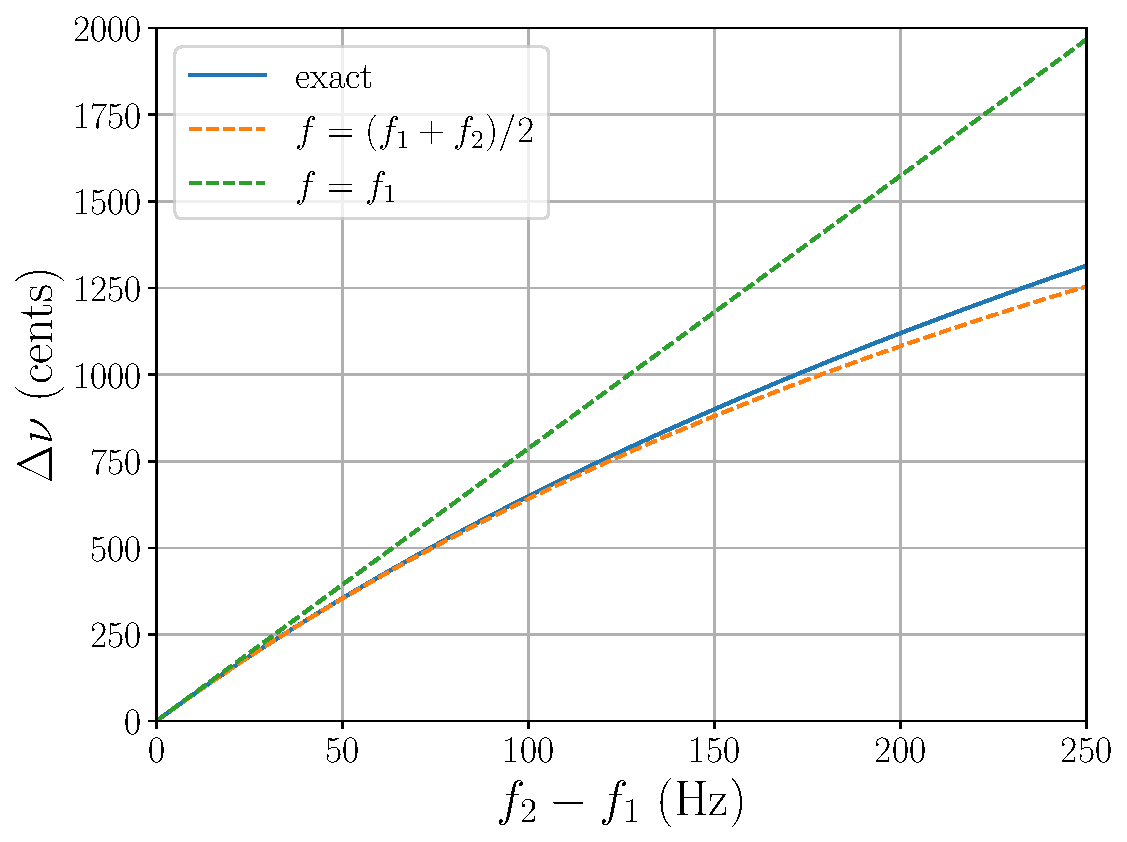
\includegraphics[width=6.5in]{../figures/diff_pitch}
    \caption{\label{fig:diff_pitch} Plot of $\Delta \nu$ for $f_1 = A_3 = 220$~Hz and $f_2$ varying from $A_3$ to $A_4 + 30 \textrm{ Hz} = 450$~Hz. We compare two different definitions of $f$ in \eqn{cents_approx}: the average of $f_1$ and $f_2$, and simply $f = f_1$. Using the average frequency leads to a significantly better approximation.}
\end{figure}
  

We present the basics of our model of classical guitar strings in \sct{model}, following the pioneering work of G.\ Byers~\cite{ref:byers1996cgi,ref:byersweb}. We begin with a new expression for the allowed vibration frequencies of a stiff string, derived in \app{freq} under the assumption that the boundary conditions at the saddle and the nut are not symmetric. We then include a discussion of the four contributions to frequency shifts and errors of non-ideal strings pressed behind a fret: the change in the resonant length of the string; a decrease in the linear mass density and an increase in the tension of the string; and the mechanical stiffness of the resonating string. Our goal is to simplify the equations through Taylor series expansions to allow an intuitive picture of the string's behavior to emerge. We offer an empirical reason to doubt the need for a complicated model of string fretting, and we explore this argument in greater detail in \app{fret}. In \sct{exp}, we suggest a simple experiment to estimate the response of the string's tension to the change in length caused by fretting, and we demonstrate the idea using a normal-tension string set on an Alhambra 8P guitar (as well as other string sets in \app{specs}). Then, in \sct{comp}, we use these estimates to demonstrate a straightforward analytic approach to compensating the errors in a guitar string, relying on a method --- described in \app{rms} --- to minimize the root-mean-squared (RMS) frequency deviation at each fret. Finally, in \sct{temp} we discuss a collaboration of guitar manufacturer and musician to temper the guitar using harmonic tuning and optimize it for a particular piece.

This document -- as well as the Python computer code needed to reproduce the figures -- is available at GitHub~\cite{ref:github2021rgb}. 
 %%%%%%%%%%%%%%%%%%%%%%%%%%%%%%%%%%%%%%%%%%%%%%%%%%%%%%%%%%%%%%%%%%%%%%%%%%%%%%
%
% Section file included in main project file using \input{}
%
% Assumes that LaTeX2e macros and packages defined in cg_comp.sty are
%   available
%
%%%%%%%%%%%%%%%%%%%%%%%%%%%%%%%%%%%%%%%%%%%%%%%%%%%%%%%%%%%%%%%%%%%%%%%%%%%%%%

 \section{Simple Model of Guitar Intonation\label{sct:model}}

Fundamental frequency of a string~\cite{ref:morse1981vas,ref:morse1981vsa}:
 \begin{equation} \label{eqn:f_0_def}
f_0 = \frac{1}{2\, L_0}\, \sqrt{\frac{T_0}{\mu_0}}\, ,
 \end{equation}
where $L_0$ is the length of the free (unfretted) string from the saddle to the nut, $T_0$ is the tension in the free string, and $\mu_0 \equiv M / L_0$ is the linear mass density of a free string of mass $M$.

 \begin{equation} \label{eqn:f_0_stiff}
f_0 = \frac{1}{2\, L_0}\, \sqrt{\frac{T_0}{\mu_0}} \left[ 1 + B_0 + \left(1 + \frac{\pi^2}{8}\right) B_0^2 \right]\, ,
 \end{equation}
where $B_0$ is a ``string stiffness parameter.'' For a uniform string with a cylindrical cross section, $B_0$ given by~\cite{ref:morse1981vsb}
 \begin{equation} \label{eqn:b_def}
B_0 \equiv \sqrt{\frac{\pi\, R^4 E}{T_0\, L_0^2}}\, ,
 \end{equation}
where $R$ is the radius of the string and $E$ is Young's modulus (or the modulus of elasticity). For a typical nylon guitar string with $E \approx 2 - 4$~GPa, $T_0 \approx 50 - 70$~N, $R \approx 0.35 - 0.51$~mm, and $L_0 \approx 650$~mm, we have $B_0 \approx 0.007 - 0.026$, indicating that the corrections in \eqn{f_0_stiff} are not significant.

Throughout this work, we will use \emph{cents} to describe small differences in pitch~\cite{ref:durfee2015pms}. One cent is one one-hundredth of a 12-TET half step, so that there are 1200~cents per octave. The difference in pitch between frequencies $f_1$ and $f_2$ is therefore defined as
 \begin{equation} \label{eqn:cents_def}
\Delta \nu \equiv 1200\, \log_2\left(\frac{f_2}{f_1}\right)\, .
 \end{equation}
We define $f \equiv (f_1 + f_2) / 2$ and $\Delta f \equiv f_2 - f_1$. Then
 \begin{equation} \label{eqn:cents_approx}
\Delta \nu = 1200\, \log_2\left(\frac{f + \Delta f / 2}{f - \Delta f /2}\right) \approx \frac{1200}{\ln 2}\, \frac{\Delta f}{f}\, ,
 \end{equation}
where the last approximation applies when $\Delta f \ll f$. An experienced guitar player can distinguish beat notes with a difference frequency of $\Delta f \approx 1$~Hz, which corresponds to 8~cents at $A_2$ ($f = 220$~Hz) or 5~cents at $E_4$ ($f = 329.63$~Hz).

 \begin{figure}
  \centering
  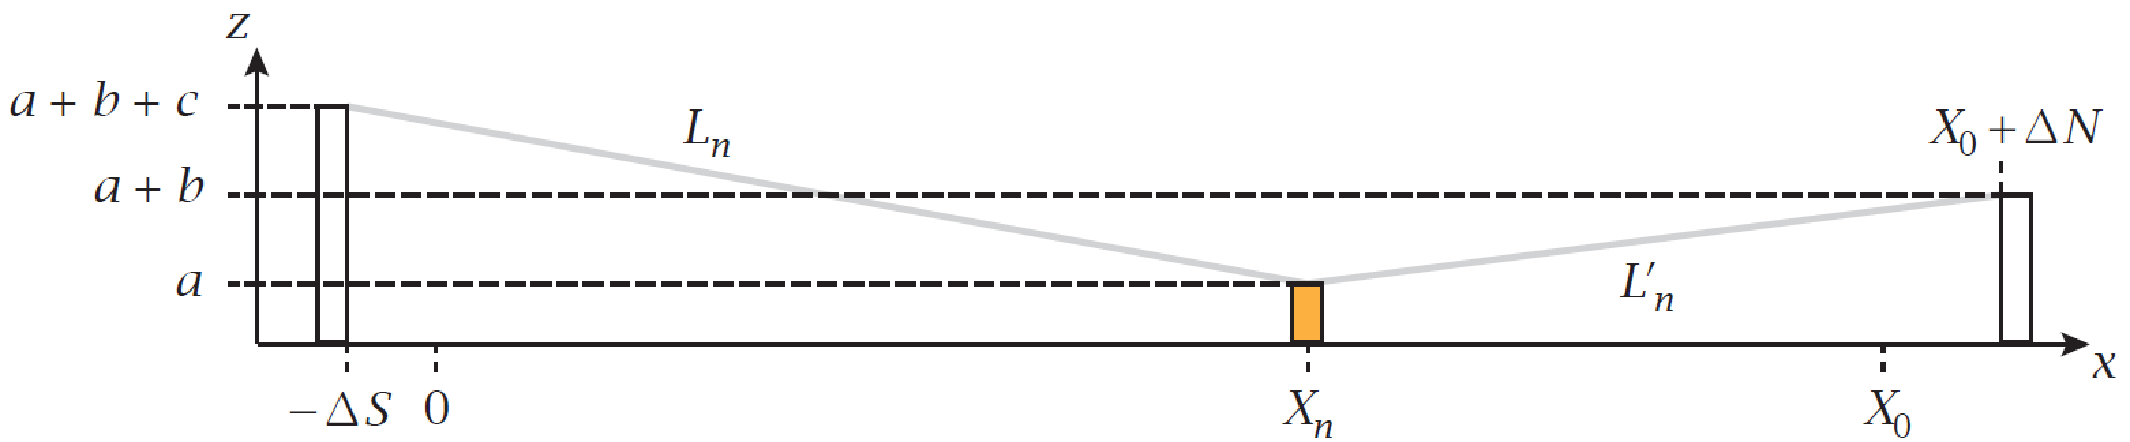
\includegraphics[width=6.0in]{figures/guitar_schematic}
  \caption{\label{fig:guitar_schematic} A simple (side-view) schematic of the classical guitar used in this model. The scale length of the guitar is $X_0$, but we allow the edges of both the saddle and the nut to be set back an additional distance $\Delta S$ and $\Delta N$, respectively. The location on the $x$-axis of the center of the $n^\textrm{th}$ fret is $X_n$. In the $z$ direction, $z = 0$ is taken as the surface of the fingerboard; therefore the height of each fret above the fingerboard is $a$, the height of the nut is $a + b$, and the height of the saddle is $a + b + c$. $L_n$ is the \emph{resonant length} of the string from the saddle to the center of fret $n$, and $L^\prime_n$ is the length of the string from the fret to the nut.}
 \end{figure}

Our model begins with the schematic of the guitar shown in \fig{guitar_schematic}. The scale length of the guitar is $X_0$, but we allow the edges of both the saddle and the nut to be set back an additional distance $\Delta S$ and $\Delta N$, respectively. The location on the $x$-axis of the center of the $n^\textrm{th}$ fret is $X_n$. In the $z$ direction, $z = 0$ is taken as the surface of the fingerboard; the height of each fret is $a$, the height of the nut is $a + b$, and the height of the saddle is $a + b + c$. $L_n$ is the \emph{resonant length} of the string from the saddle to the center of fret $n$, and $L^\prime_n$ is the length of the string from the fret to the nut. The total length of the string is defined as $\mathcal{L}_n \equiv L_n + L^\prime_n$. For reasons discussed below, we have not adopted a more complicated fretting model~\cite{ref:byers1996cgi,ref:varieschi2010icf}. We start with the simple form of the fundamental frequency of a string given by \eqn{f_0_def}, and apply it to the frequency of a string pressed just behind the $n^\mathrm{th}$ fret:
 \begin{equation} \label{eqn:f_n_def}
f_n = \frac{1}{2\, L_n}\, \sqrt{\frac{T_n}{\mu_n}}\, ,
 \end{equation}
where $T_n$ and $\mu_n$ are respectively the tension and linear mass density of the fretted string. We note that $T_n$ and $\mu_n$ depend on $\mathcal{L}_n$, the \emph{total} length of the fretted string from the saddle to the nut. Ideally, in the 12-TET equal-temperament system~\cite{ref:durfee2015pms},
 \begin{equation} \label{eqn:f_n_tet}
f_n = \gamma_n\, f_0\, , \qquad \textrm{(12-TET~ideal)}
 \end{equation}
where
 \begin{equation} \label{eqn:gamme_n_def}
\gamma_n \equiv 2^{n / 12}\, .
 \end{equation}
Therefore, the error interval expressed in cents is given by
 \begin{equation}\label{eqn:error_def}
 \begin{split}
\Delta \nu_n &= 1200\, \log_2\left( \frac{f_n}{\gamma_n\, f_0} \right) \\
&= 1200\, \log_2 \left( \frac{L_0}{\gamma_n\, L_n}\, \sqrt{\frac{\mu_0}{\mu_n}\, \frac{T_n}{T_0}}\, \right) \\
&= 1200\, \log_2 \left( \frac{L_0}{\gamma_n\, L_n} \right) + 600\, \log_2 \left(  \frac{\mu_0}{\mu_n} \right) + 600\, \log_2 \left( \frac{T_n}{T_0} \right)\, .
 \end{split}
 \end{equation}

The final form of \eqn{error_def} makes it clear that --- for nylon guitar strings --- there are three contributions to intonation:
 \begin{enumerate}
  \item
   \emph{Resonant Length}: The first term represents the error caused by the increase in the length of the fretted string $L_n$ compared to the ideal length $X_n$, which would be obtained if $b = c = 0$ and $\Delta S = \Delta N = 0$.
  \item
   \emph{Linear Mass Density}: The second term is the error caused by the reduction of the linear mass density of the fretted string. This effect will depend on the \emph{total} length of the string, given by $\mathcal{L}_n = L_n + L^\prime_n$.
  \item
   \emph{Tension}: The third (and most complex) term is the error caused by the \emph{increase} of the tension in the string caused by the stress and strain applied to the string by fretting. This effect will also depend on the total length of the string $\mathcal{L}_n$.
 \end{enumerate}
We will discuss each of these three sources of error in turn below.

 \subsection{Resonant Length Error}
We can estimate the first term in the last line of \eqn{error_def} by referring to \fig{guitar_schematic} and computing the resonant length $L_n$. We find:
 \begin{equation}
L_n = \begin{cases}
\sqrt{\left(X_0 + \Delta S + \Delta N\right)^2 + c^2}\, , & n =  0 \\
\sqrt{\left(X_n + \Delta S\right)^2 + (b + c)^2}\, . & n \ge 1
 \end{cases}
 \end{equation}
When $b + c \ll X_0$ and the guitar has been manufactured such that $X_n = X_0 / \gamma_n$, we can approximate $L_n$ by
 \begin{equation} \label{eqn:l_n_approx}
L_n \approx \begin{cases}
X_0 + \Delta S + \Delta N + c^2/2\, X_0\, , & n =  0 \\
\gamma_n^{-1} \left\{X_0 + \gamma_n \Delta S + \left[\gamma_n (b + c)\right]^2/2\, X_0\right\}\, . & n \ge 1
 \end{cases}
 \end{equation}
 Suppose that $X_0 = 650$~mm, $b + c = 5$~mm, and $n = 12$ (i.e., $\gamma_{12} = 2$). Then $\left[\gamma_n (b + c)\right]^2/2\, X_0 < 0.1$~mm, and it's clear that we can neglect the terms here that depend on $b$ and/or $c$. Then the resonant length error is approximately
  \begin{equation}
  1200\, \log_2 \left( \frac{L_0}{\gamma_n\, L_n} \right) \approx -\frac{1200}{\ln(2)}\, \frac{\left(\gamma_n - 1\right) \Delta S - \Delta N}{X_0}
  \end{equation}
If the guitar is uncompensated, so that $\Delta S = \Delta N = 0$, this error is negligible. In fact, for most classical guitars and strings, it is much less than 1~cent because the impact of $b$ and $c$ on $L_n$ is quadratic and therefore very small. But, with $\Delta S > 0$ and $\Delta N < 0$, we can \emph{increase} the magnitude of this ``error'' and cause the frequency to shift lower. We'll see that this is our primary method of compensation. \red{TBD: Add a figure here?}

Previous studies of guitar intonation and compensation have chosen to include the apparent increase in length of the string caused by both the depth of the fretting action \red{(Matt: Is this the right term?)} and the shape of the fretted string under the finger~\cite{ref:byers1996cgi,ref:varieschi2010icf}. As the string is initially pressed to the fret, the total length $\mathcal{L}_n$ increases and causes the tension in the string --- which is clamped at the saddle and the nut --- to increase. As the string is pressed further, does the additional deformation of the string increase its tension (throughout the resonant length $L_n$)? There are at least two purely empirical reasons to doubt this hypothesis. First, we can mark a string (with a fine-point felt pen) above a particular fret and then observe the mark with a magnifying glass. As the string is pressed all the way to the finger board, the mark does not move perceptibly --- it has become effectively \emph{clamped} on the fret. Second, we can use either our ears or a simple tool to measure frequencies~\cite{ref:pgtweb} to listen for a shift as we use different fingers and vary the fretted depth of a string. The apparent modulation is far less than would be obtained by classical vibrato, so we assume that once the string is minimally fretted the length(s) can be regarded as fixed. (If this were not the case, then fretting by different people or with different fingers, at a single string or with a barre, would cause additional, varying frequency shifts that would be audible and difficult to compensate.)

 \subsection{Linear Mass Density Error}
As discussed above, the linear mass density $\mu_0$ of an unfretted string is simply the total mass $M$ of the string clamped between the saddle and the nut divided by the length $L_0$. Similarly, the mass density $\mu_n$ of a string held onto fret $N$ is $M/\mathcal{L}_n$. Therefore
 \begin{equation}
\frac{\mu_0}{\mu_n} = \frac{\mathcal{L}_n}{L_0} = 1 + \frac{\mathcal{L}_n - L_0}{L_0}\, .
 \end{equation}
Since we expect that $(\mathcal{L}_n - L_0)/L_0 \ll 1$, we can approximate the second term in the final line of \eqn{error_def} as
 \begin{equation}
600\, \log_2 \left(  \frac{\mu_0}{\mu_n} \right) \approx \frac{600}{\ln(2)}\, \frac{\mathcal{L}_n - L_0}{L_0}
 \end{equation}

Referring to \fig{guitar_schematic}, we see that $\mathcal{L} = L_n + L^\prime_n$, and we calculate $L^\prime_n$ as
 \begin{equation}
L^\prime_n = \begin{cases}
0\, , & n =  0 \\
\sqrt{\left(X_0 - X_n + \Delta N\right)^2 + b^2}\, . & n \ge 1
 \end{cases}
 \end{equation}
Assuming that $b^2 \ll X_0 - X_n + \Delta N$, we expand the $n \ne 1$ expression to obtain
 \begin{equation}
L^\prime_n \approx X_0 - X_n + \Delta N + \frac{b^2}{2 \left(X_0 - X_n + \Delta N\right)}
 \end{equation}
Therefore, since \eqn{l_n_approx} gives $L_n \approx X_n + \Delta S$, we have for $n \ne 1$
 \begin{equation}
 \begin{split}
\mathcal{L}_n &= L_n + L^\prime_n \approx X_0 + \Delta S + \Delta N + \frac{b^2}{2 \left(X_0 - X_n + \Delta N\right)} \\
&\approx L_0 + \frac{b^2}{2 \left(X_0 - X_n + \Delta N\right)}\, ,
 \end{split}
 \end{equation}
and
 \begin{equation}
600\, \log_2 \left( \frac{\mu_0}{\mu_n} \right) \approx \frac{600}{\ln(2)}\, \frac{b^2}{2\, L_0 \left(X_0 - X_n + \Delta N\right)}\, .
 \end{equation}
This error is generally quite small. Suppose that $b = 3$~mm, $X_0 = 650$~mm, $n = 1$, $X_1 = 2^{-1/12}\, X_0 = 613.5$~mm, and $\Delta N = 0$. Then the error is less than 0.2~cents, and will be even smaller for $n \ge 2$.
 %%%%%%%%%%%%%%%%%%%%%%%%%%%%%%%%%%%%%%%%%%%%%%%%%%%%%%%%%%%%%%%%%%%%%%%%%%%%%%
%
% Section file included in main project file using \input{}
%
% Assumes that LaTeX2e macros and packages defined in cg_comp.sty are
%   available
%
%%%%%%%%%%%%%%%%%%%%%%%%%%%%%%%%%%%%%%%%%%%%%%%%%%%%%%%%%%%%%%%%%%%%%%%%%%%%%%

 \section{Experimental Estimate of the String Constant\label{sct:exp}}

 \begin{figure}
  \centering
  \begin{subfigure}[b]{0.45\textwidth}
      \centering
      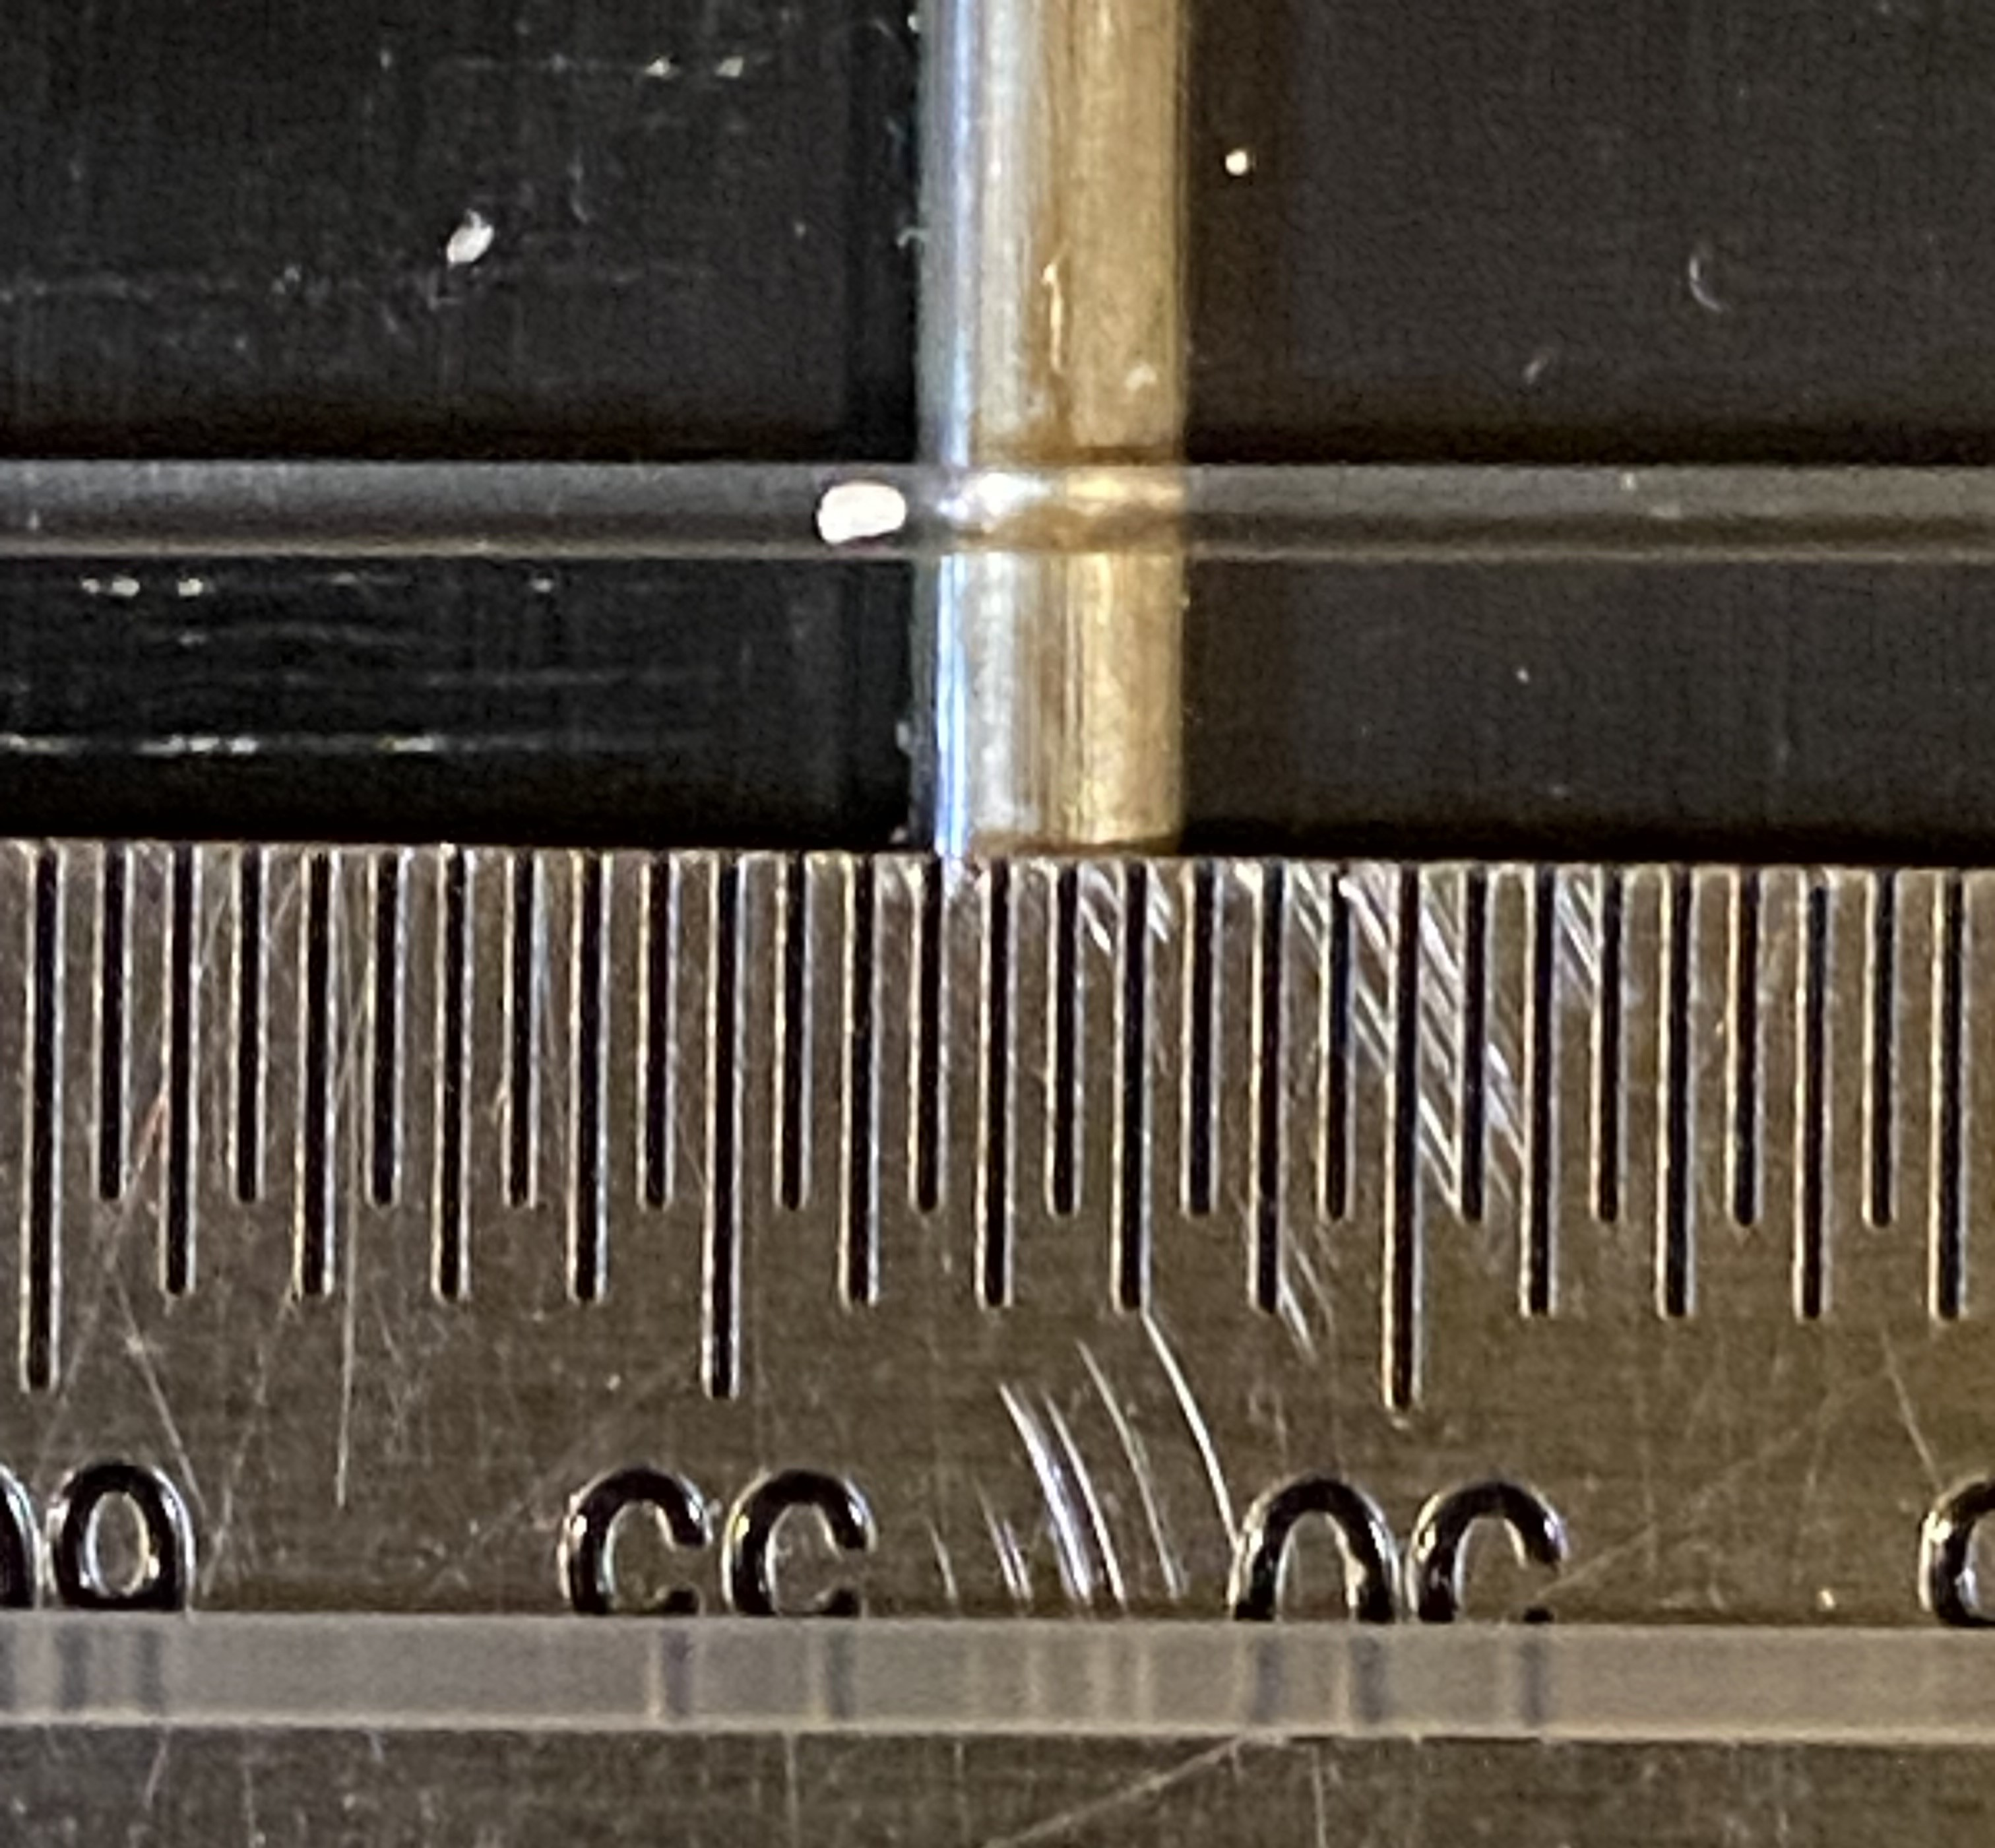
\includegraphics[width=3.0in]{../figures/exp_dx1.jpg}
      \caption{$\Delta x_1$}
      \label{fig:exp_dx1}
  \end{subfigure}
  \hspace{0.25in}
  \begin{subfigure}[b]{0.45\textwidth}
      \centering
      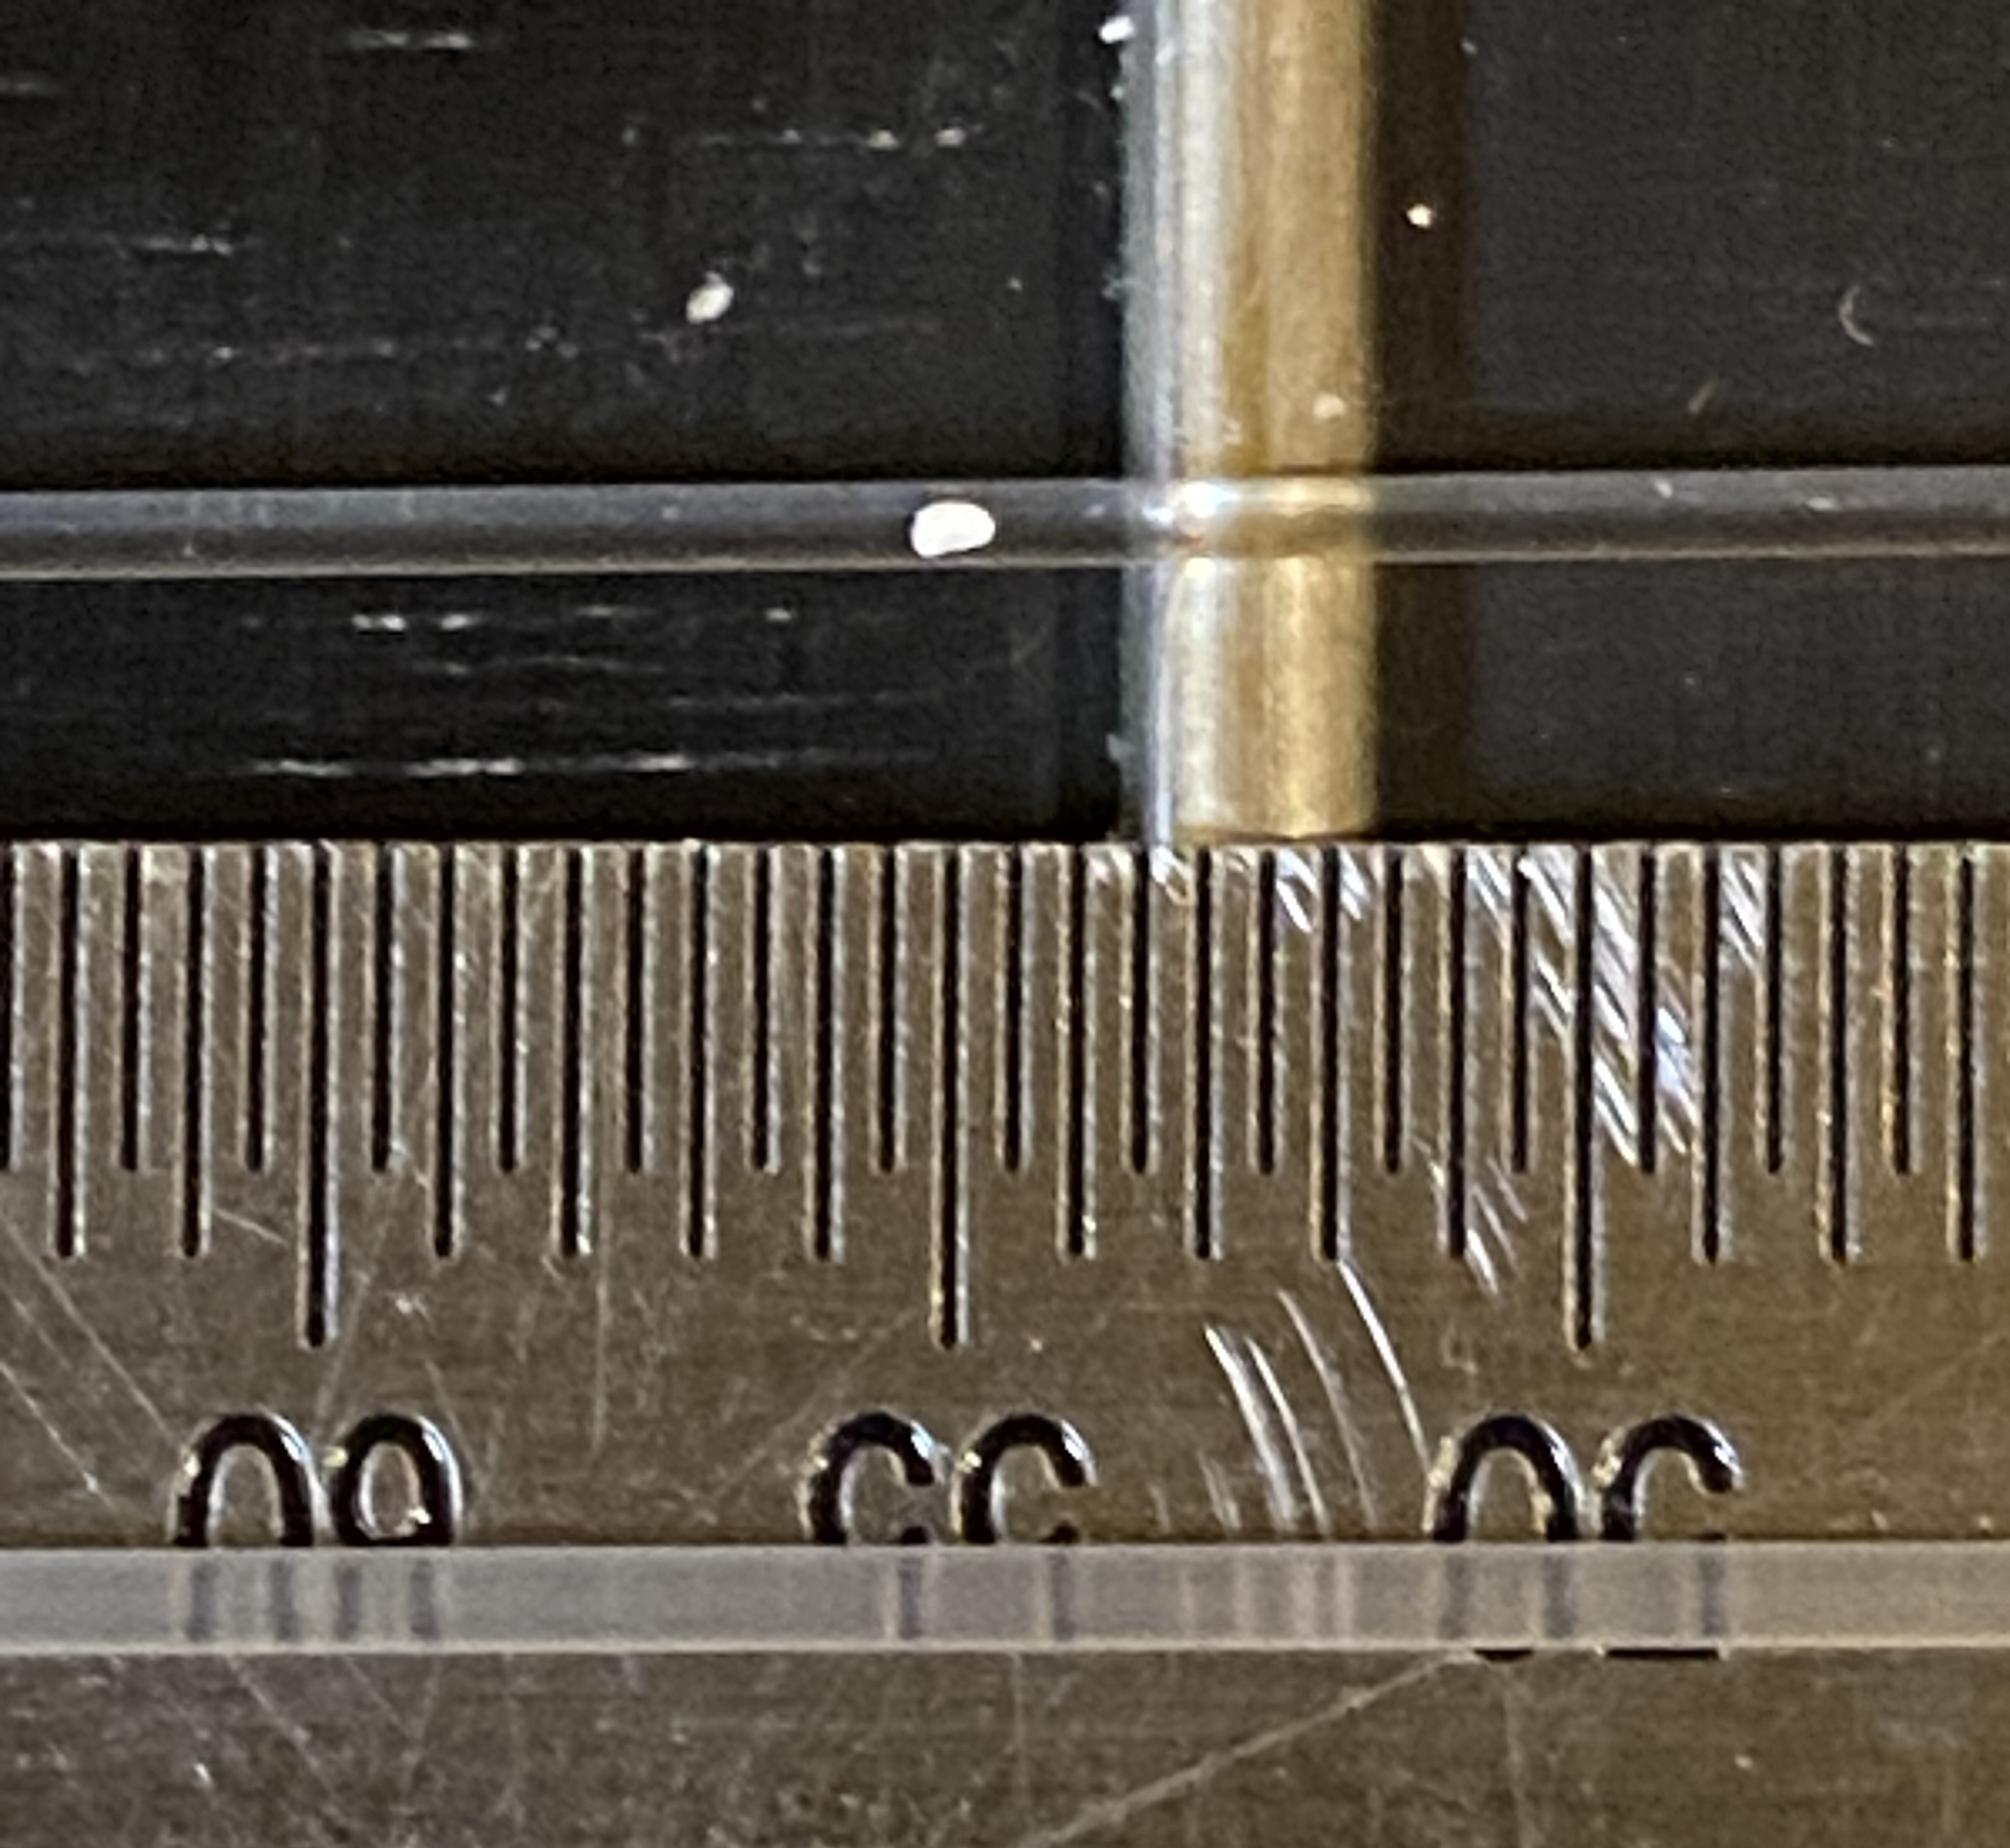
\includegraphics[width=3.04in]{../figures/exp_dx2.jpg}
      \caption{$\Delta x_2$}
      \label{fig:exp_dx2}
  \end{subfigure}
  \caption{\label{fig:exp_dx} Two examples of displacement measurements of a small deposit of white correction fluid relative to a D'Addario string-depth gauge marked in half-millimeter increments.}
\end{figure}

\begin{table}
  \centering
  \caption{\label{tbl:ej45_mks} String specifications for the D'Addario Pro-Arte Nylon Classical Guitar Strings -- Normal Tension (EJ45). The corresponding scale length is 650~mm.}
  \begin{tabular}{cccccc}
\toprule
String & Note & Radius (mm) & Density ($\times 10^{-7}$ kg/mm) & Tension (N) \\
\midrule
J4501 & E$_{4}$ & 0.356 & 3.74 & 68.6 \\
J4502 & B$_{3}$ & 0.409 & 5.05 & 52.0 \\
J4503 & G$_{3}$ & 0.512 & 8.36 & 54.3 \\
J4504 & D$_{3}$ & 0.368 & 19.21 & 70.0 \\
J4505 & A$_{2}$ & 0.445 & 32.90 & 67.3 \\
J4506 & E$_{2}$ & 0.546 & 54.72 & 62.8 \\
\bottomrule
\end{tabular}


\end{table}%

It is relatively easy to measure \emph{in situ} the value of $R$ (and therefore $\kappa$ and $B_0$) for any guitar string with the aid of a  device that can measure frequency~\cite{ref:pgtweb}, a simple ruler with fine markings (e.g., a string depth gauge), a magnifying glass or camera with a macro mode, and white correction fluid. For example, in \fig{exp_dx} we show photographs of the nylon normal-tension first string on an Alhambra 8P classical guitar. By depositing a small sample of white correction fluid on the string, we can measure small displacements within 0.125~mm against a string-depth gauge marked in half-millimeter increments. Then we can pluck the open string and measure its vibration frequency. We found that significantly stretching a string that had settled into equilibrium could result in a nonlinear reduction in $\Delta f/\Delta L$, so prior to our measurements we tuned each string down one whole step. The string stretches uniformly along its length, so at any position $x$ the relative displacement $\Delta x/x$ should be invariant. We chose to work near the first fret, which is located about 614~mm from the saddle, and we typically made seven measurements of displacement over a 3~mm range, as well as the corresponding frequencies.

\begin{figure}
  \centering
  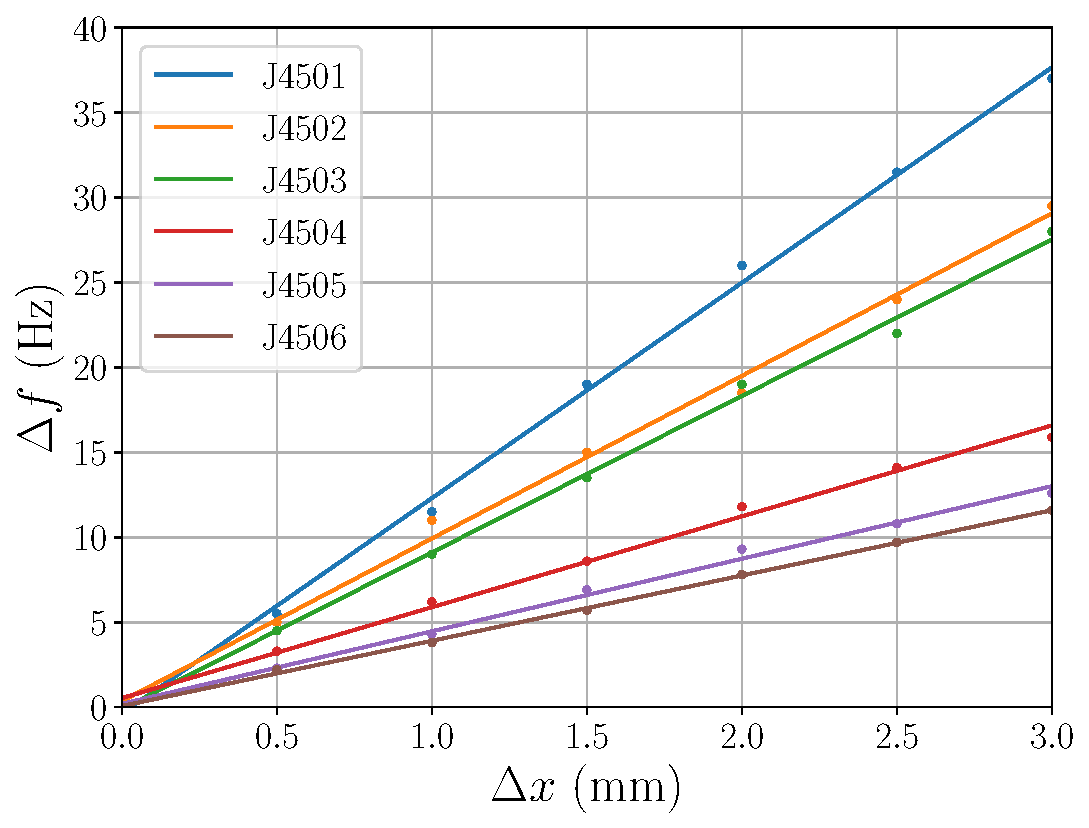
\includegraphics[width=5.0in]{../figures/fit_ej45}
  \caption{\label{fig:fit_ej45} Results of experiments to measure $R$ for each string in the D'Addario Pro-Arte Nylon Classical Guitar Strings -- Normal Tension (EJ45) set. The points represent the measurement data, while the lines are the results of linear least-squares fits to that data.}
 \end{figure}

For example, we began with a normal-tension nylon classical string set~\cite{ref:daddariostcweb} with the specifications listed in \tbl{ej45_mks} using metric units.\footnote{Note that the correct unit of force in the metric system is Newtons (N), rather than kilograms, which is a unit of mass. In the British Imperial measurement system, the common units of mass are known as the ``slug'' and the ``blob.''} In \fig{fit_ej45}, we plot our measurements of $\Delta f$ as a function of the displacement $\Delta x$ relative to the frequency of the string when $\Delta x = 0$. We then performed a least-squares fit to a straight line~\cite{ref:bevington2003dre} (also shown in \fig{fit_ej45}), determined the derivative $\Delta f / \Delta L$, and then computed $R$ using \eqn{r_def} with $L = 614$~mm and $f$ defined as the average frequency over the range. The results are shown in \tbl{ej45_props}. Here $\sigma$ is the covariant (diagonal) uncertainty in $R$ (so that, for example, the first string in the table has $R = 23.6 \pm 0.5$), and $\kappa = 2 R + 1$. We also estimate an effective modulus of elasticity $E$ from \eqn{kappa_def}, expressed in units of gigapascals (1 GPa = $10^9$~N/m$^2$.). Similar measurements and results for other string sets are provided in \app{specs}. Note --- as predicted in \sct{tot_freq_shift} and shown in \fig{hist_r} --- the expectation that the guitar will be \emph{tunable} results in $R$ values of manufactured strings that are in the range $20 - 30$. The still more important requirement that the guitar be \emph{playable} leads us to the discussion of compensation in the next section.

% First, we tune the open string to the correct 12-TET frequency. Then, we select a fret $n$, and measure the frequency deviation $\Delta \nu_n$ of the fretted string while muting the other strings to eliminate sympathetic vibrations. If we solve \eqn{b_0_kappa} for $\kappa$ and then substitute the result into \eqn{error_tot}, we find
% \begin{equation} \label{eqn:root_kappa_quad}
%   \alpha\, B_0^2 + \beta\, B_0 - \xi = 0\, ,
% %  \alpha\, \kappa + \beta\, \sqrt{\kappa} - \xi = 0\, ,
% \end{equation}
% where we have included the quadratic bending stiffness term, and defined the coefficients
% \begin{subequations}
%   \begin{align}
%     % \alpha &\equiv \half \left[ Q_n + \left(\gamma_n^2 - 1\right)\left(1 + \pi^2\right)\left(\frac{\rho}{2\, L_0}\right)^2 \right]\, , \\
%     % \beta &\equiv \left(\gamma_n - 1\right)\, \frac{\rho}{2\, L_0}\, , \nd \\
%     % \xi &\equiv \frac{\ln(2)}{1200}\, \Delta \nu_n + \frac{\left(\gamma_n - 1\right) \Delta S - \Delta N}{X_0}\, .
%     \alpha &\equiv \half \left[ \left(\frac{2\, L_0}{\rho}\right)^2 Q_n + \left(\gamma_n^2 - 1\right)\left(1 + \pi^2\right) \right]\, , \\
%     \beta &\equiv \gamma_n - 1\, , \nd \\
%     \xi &\equiv \frac{\ln(2)}{1200}\, \Delta \nu_n + \frac{\left(\gamma_n - 1\right) \Delta S - \Delta N}{X_0}\, .
% \end{align}
% \end{subequations}
% \Eqn{root_kappa_quad} is quadratic in $B_0$, with the solution
%  \begin{equation} \label{eqn:root_kappa_soln}
% B_0 = \frac{\sqrt{\beta^2 + 4\, \alpha\, \xi} - \beta}{2\, \alpha} \approx \frac{\xi}{\beta}\, ,
%  \end{equation}
% where we have chosen the positive root to ensure that $B_0 > 0$, and the final approximate expression on the \rhs applies when $\beta^2 \gg 4\, \alpha\, \xi$.

% We've used this approach to estimate $\kappa$ and $R$ of different string sets on the Alhambra 8P classical guitar, which has $X_0 = 650$~mm, $c = 3.5$~mm, $\Delta S = 1.5$~mm, and $\Delta N = 0.0$~mm. At the nut, $b = 1.0$~mm, but the height of the fret board decreases roughly linearly further toward the saddle, effectively increasing $b$. We estimate that $d b / d x \approx -0.0034$, so that $b$ has increased to 2.0~mm at the 12$^{\text{th}}$ fret. . In \tbl{ej45_props}, we list the frequency deviation from 12-TET at the 12$^{\text{th}}$ fret for each string in this set, as well as the corresponding estimates of $\kappa$, $R$, $E$, and $B_0$, computed from \eqn{root_kappa_soln}, \eqn{r_def}, \eqn{kappa_def}, and \eqn{b_0_kappa}, respectively.

\begin{table}%[htbp]
  \centering
  \caption{\label{tbl:ej45_props} Derived physical properties of the D'Addario Pro-Arte Nylon Classical Guitar Strings -- Normal Tension (EJ45). The corresponding scale length is 650 mm.}
  \begin{tabular}{cccccc}
\toprule
String & $R$ & $\sigma$ & $\kappa$ & $B_0$ & $E$ (GPa) \\
\midrule
J4501 & 23.6 & 0.5 & 48.2 & 0.00190 & 8.33 \\
J4502 & 23.8 & 0.7 & 48.6 & 0.00219 & 4.81 \\
J4503 & 28.8 & 0.7 & 58.7 & 0.00302 & 3.87 \\
J4504 & 22.4 & 0.8 & 45.7 & 0.00192 & 7.51 \\
J4505 & 23.8 & 0.8 & 48.6 & 0.00238 & 5.27 \\
J4506 & 28.6 & 0.4 & 58.2 & 0.00321 & 3.90 \\
\bottomrule
\end{tabular}


\end{table}%

\begin{figure}
  \centering
  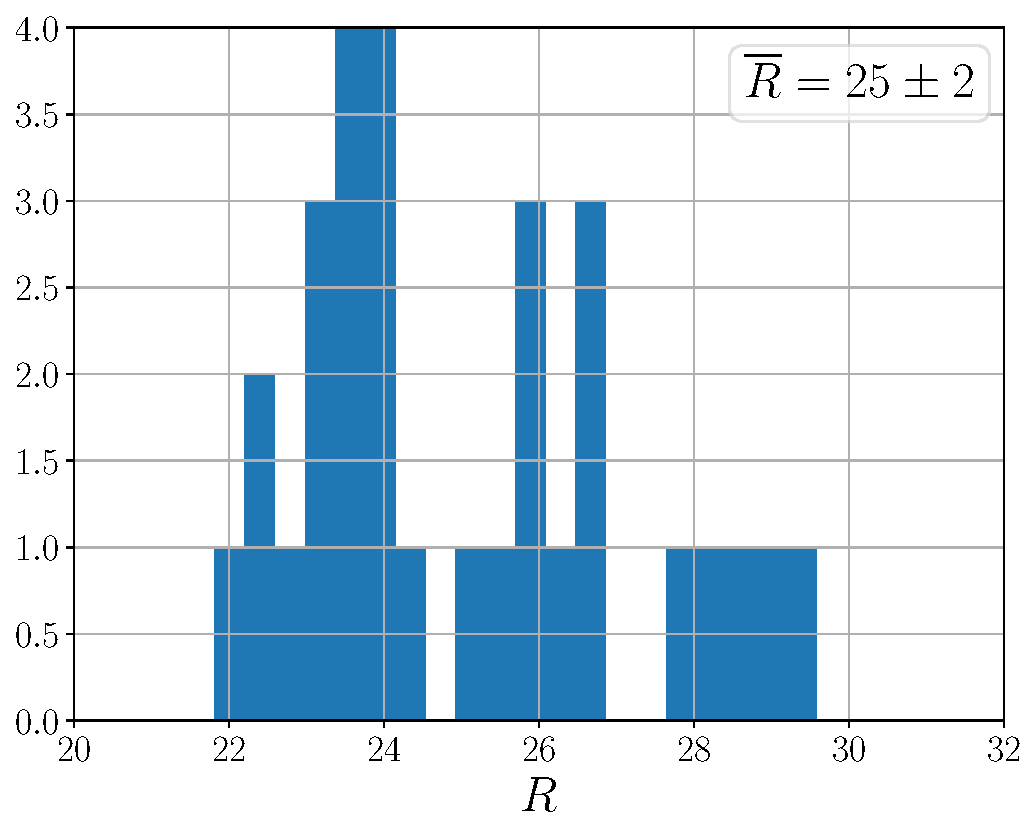
\includegraphics[width=5.0in]{../figures/hist_r}
  \caption{\label{fig:hist_r} A histogram of the parameter $R$ for all strings \emph{except} those in the nylon light tension set presented in \app{specs_ltn}, which seem to have anomalously high values.}
\end{figure}

\begin{figure}
  \centering
  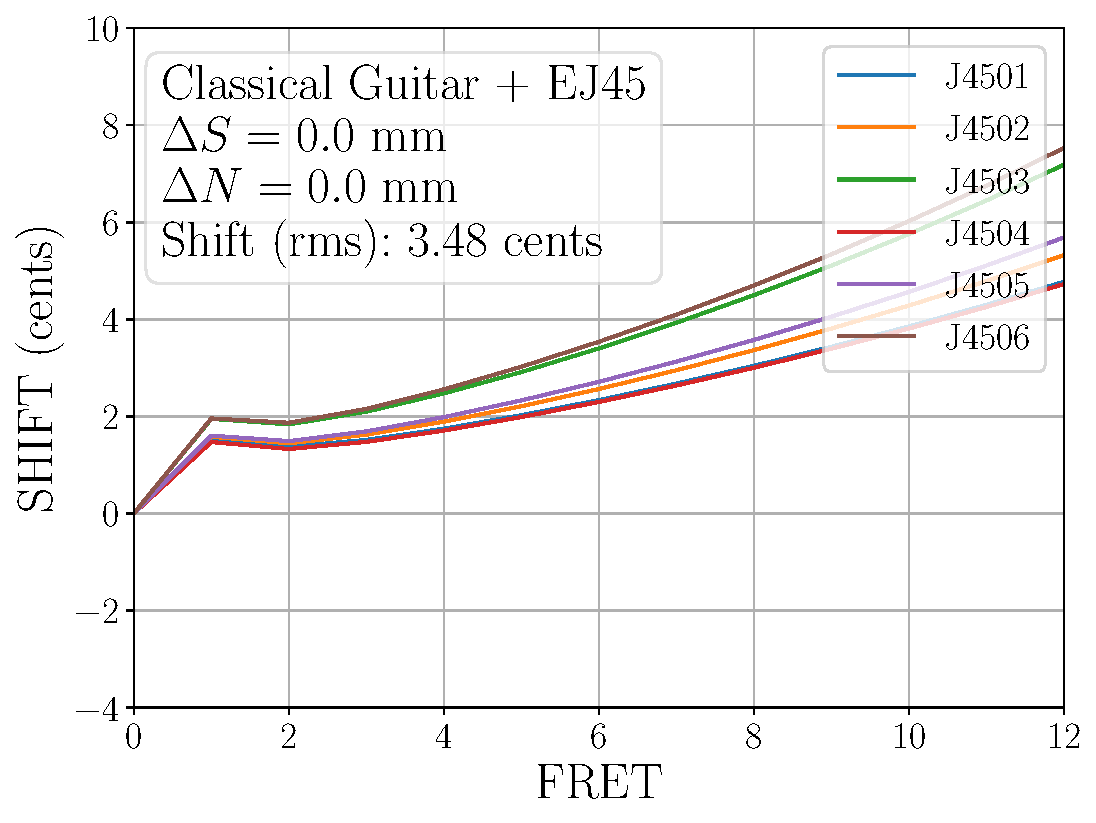
\includegraphics[width=5.0in]{../figures/shift_classicalguitar_ej45_null}
  \caption{\label{fig:shift_classicalguitar_ej45_null} Frequency errors for an uncompensated Classical Guitar with normal tension nylon strings (D'Addario EJ45).}
\end{figure}

Adopting these physical properties of the normal string set and applying them to a computation of the frequency deviations for our standard classical guitar, we obtain the predictions shown in \fig{shift_classicalguitar_ej45_null} using \eqn{error_def}. Anticipating our treatment of exact compensation in \sct{comp} and \app{rms}, we compute the root-mean-squared (RMS) average of the frequency deviations for each string. This mean (over the first 12 frets) can be computed by squaring the frequency deviations shown in \fig{shift_classicalguitar_ej45_null}, averaging those values, and then taking the square root of the result.

%Recall how we introduced this concept in \sct{model_tension}: increasing the tension by a quantity $\Delta T$ causes a shift in the frequency of a guitar string by $\Delta \nu$ in cents. Although we were considering fretted strings when we derived \eqn{error_def}, the terms in that equation can be generalized to describe the case of an open string that has been stretched longitudinally. Suppose that we continue to clamp the string at the saddle and the nut, but that we tighten the tuning gear to stretch that string's length by an amount $\Delta L$. The change in the string's frequency due to the change in the open resonant length is zero, because $L_0 / \gamma_0 L_0 = 1$. The linear mass density of the string is smaller now because there is less material between the saddle and the nut, causing the frequency shift (in cents)
% \begin{equation}
%600\, \log_2 \left(  \frac{\mu}{\mu + \Delta \mu} \right) \approx \frac{600}{\ln(2)}\, \frac{\Delta L}{L}\, ,
% \end{equation}
%where $L$ is the initial length of the string. Finally, the tension in the string increases by $\Delta T$ due to the elastic properties of the string. Following the discussion in \sct{model_tension}, the corresponding frequency shift  is
% \begin{equation}
%600\, \log_2 \left(  \frac{T + \Delta T}{T} \right) \approx \frac{600}{\ln(2)}\, \frac{\Delta L}{L}\, \kappa\, ,
% \end{equation}
%where $T$ is the initial tension of the string. Therefore, the total frequency shift of the open string caused by a change $\Delta L$ in the string's length is
% \begin{equation}
%\Delta \nu \approx \frac{600}{\ln(2)}\, \frac{\Delta L}{L}\, (\kappa + 1)\, ,
% \end{equation}
%characterizing the string frequency's response to a change in length. It is dominated by the change in the tension of the string, and given $R$ we can quickly determine $\kappa$.
%
%
%Solving this expression for the string constant, we find
% \begin{equation}
%\kappa = \frac{\ln(2)}{600}\, R - 1\, ,
% \end{equation}
%where
% \begin{equation}
%R \equiv \frac{L}{\Delta L}\, \Delta \nu
% \end{equation}
%is a parameter originally defined by Byers\footnote{Byers expressed this parameter in terms of the fractional frequency shift (in Hertz) as $R = (L/\Delta L) (\Delta f/f) \approx (\ln(2)/1200) (L/\Delta L) \Delta \nu$. Therefore, our dimensionless value of $R$ is larger than Byers' by a factor of about 1730.}~\cite{ref:byers1996cgi,ref:varieschi2010icf}.

% \begin{equation}
% \begin{split}
%L_{n \ge 1}(y) &= \sqrt{\left(X_n + \Delta S\right)^2 + (b + c)^2 + y^2} \\
%&\approx X_n + \Delta S + \frac{(b + c)^2 + y^2}{2\, X_n}\, .
% \end{split}
% \end{equation}
%
% \begin{equation}
% \begin{split}
%L^\prime_{n \ge 1}(y) &= \sqrt{\left(X_0 - X_n + \Delta N\right)^2 + b^2 + y^2} \\
%&\approx X_0 - X_n + \Delta N + \frac{b^2 + y^2}{2 \left(X_0 - X_n\right)}\, .
% \end{split}
% \end{equation}
%
% \begin{equation}
% \begin{split}
%Q_n(y) &\approx \frac{1}{2\, X_0} \left[ \frac{(b + c)^2 + y^2}{X_n} + \frac{b^2 + y^2}{X_0 - X_n} - \frac{c^2}{X_0} \right] \\
%&= Q_n(0) + \Delta Q_n(y) \, ,
% \end{split}
% \end{equation}
%where $Q_n(0)$ is given by \eqn{lambda_n_approx}, and
% \begin{equation}
%\Delta Q_n(y) \equiv \frac{1}{2 \left(\gamma_n - 1\right)}\, \left(\frac{\gamma_n\, y}{X_0}\right)^2\, .
% \end{equation}
%
%Following the same approach we used to derive \eqn{quad_shift}, we can derive the change in the total shift due to both resonant length and linear mass density for a transverse displacement $y$. To second order in $y$, we find that
% \begin{equation}
%\Delta \nu_n(y) \approx \frac{600}{\ln(2)}\, \frac{3 - 2 \gamma_n}{2 \left(\gamma_n - 1\right)}\, \left(\frac{\gamma_n\, y}{X_0}\right)^2\, .
% \end{equation}
%We have plotted this expression for the first 12 frets and $y = 5$~mm in \fig{quad_shift_factory}. This shift is quite small compared to the experimental errors we'll obtain in the shifts due to tension, and we ignore it in what follows.
%
% \begin{figure}
%  \centering
%  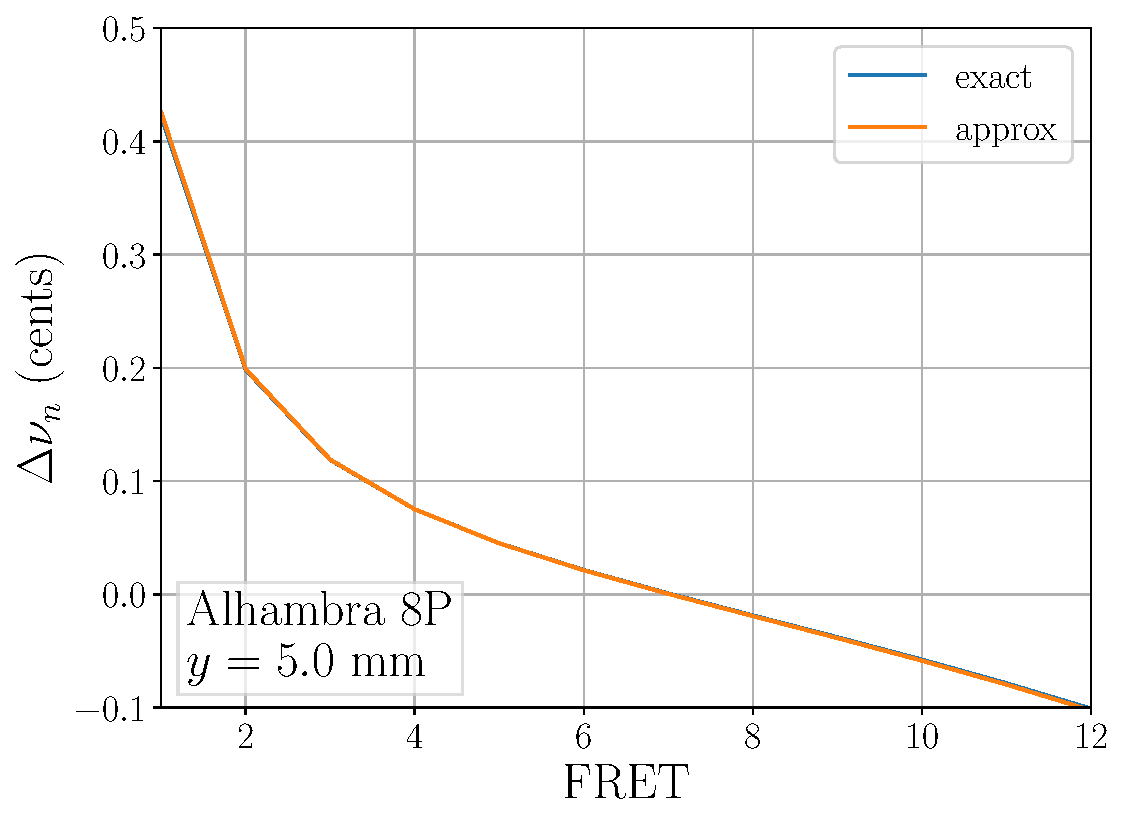
\includegraphics[width=5.0in]{figures/quad_shift_factory}
%  \caption{\label{fig:quad_shift_factory} Total frequency shift (in cents) due to resonant length and linear mass density for a transverse displacement of $y = 5$~mm. This shift is identical for each string, and should be smaller than the experimental errors we'll accumulate using our transverse displacement approach.}
% \end{figure}
%
%\begin{table}%[htbp]
%  \centering
%  \caption{\label{tbl:ej43_props} Derived physical properties of the D'Addario Pro-Arte Nylon Classical Guitar Strings -- Light Tension (EJ43). The corresponding scale length is 650 mm.}
%    \begin{tabular}{lcccc}
%    \hline \hline
%    String  & $R$ & $\kappa$ & Modulus (GPa) & Stiffness \\
%    \hline
%    J4301 & 4.39 $\times 10^{4}$ & 49.8 & 8.62 & 3.79 $\times 10^{-3}$ \\
%    J4302 & 5.02 $\times 10^{4}$ & 57.0 & 5.62 & 4.68 $\times 10^{-3}$ \\
%    J4303 & 4.79 $\times 10^{4}$ & 54.4 & 3.57 & 5.72 $\times 10^{-3}$ \\
%    J4304 & 5.02 $\times 10^{4}$ & 57.0 & 9.52 & 4.13 $\times 10^{-3}$ \\
%    J4305 & 4.39 $\times 10^{4}$ & 49.8 & 5.05 & 4.55 $\times 10^{-3}$ \\
%    J4306 & 5.27 $\times 10^{4}$ & 59.9 & 3.97 & 6.35 $\times 10^{-3}$ \\
%    \hline
%    \end{tabular}%
%  \label{tab:addlabel}%
%\end{table}%

%\begin{table}[htbp]
%  \centering
%  \caption{\label{tbl:ej45_ips} String specifications for the D'Addario Pro-Arte Nylon Classical Guitar Strings -- Normal Tension (EJ45). The corresponding scale length is 25.5~inches.}
%    \begin{tabular}{lcccc}
%    \toprule
%    String  & Note  & \multicolumn{1}{l}{Diameter (in)} & \multicolumn{1}{l}{Density (lb/in)} & \multicolumn{1}{l}{Tension (lb)} \\
%    \midrule
%    J4501 & $E_4$  & 0.0280 & $2.092 \times 10^{-5}$ & 15.3 \\
%    J4502 & $B_3$  & 0.0322 & $2.827 \times 10^{-5}$ & 11.6 \\
%    J4503 & $G_3$  & 0.0403 & $4.679 \times 10^{-5}$ & 12.1 \\
%    J4504 & $D_3$  & 0.0290 & $1.075 \times 10^{-4}$ & 15.6 \\
%    J4505 & $A_2$  & 0.0350 & $1.842 \times 10^{-4}$ & 15.0 \\
%    J4506 & $E_2$  & 0.0430 & $3.063 \times 10^{-4}$ & 14.0 \\
%    \bottomrule
%    \end{tabular}%
%\end{table}%

 %%%%%%%%%%%%%%%%%%%%%%%%%%%%%%%%%%%%%%%%%%%%%%%%%%%%%%%%%%%%%%%%%%%%%%%%%%%%%%
%
% Section file included in main project file using \input{}
%
% Assumes that LaTeX2e macros and packages defined in cg_comp.sty are
%   available
%
%%%%%%%%%%%%%%%%%%%%%%%%%%%%%%%%%%%%%%%%%%%%%%%%%%%%%%%%%%%%%%%%%%%%%%%%%%%%%%

 \section{Classical Guitar Compensation\label{sct:comp}}

As we discussed in \sct{tot_freq_shift}, \eqn{error_tot} provides a guide to how to modify our prototypical classical guitar to improve the tone of the strings shown in \fig{shift_classicalguitar_ej45_null}. We noted that the bending stiffness and the increase in string tension due to fretting sharpen the pitch, but that we can flatten it with a positive saddle setback and negative nut setback. As in \fig{uncomp}, let's choose the guitar and string properties listed in \tbl{mcg_specs} and \tbl{string_specs}. In this case, \Fig{comp_dsdn} shows that increasing the saddle setback tends to rotate the pitch curve clockwise, and increasing the magnitude of the negative nut setback displaces the pitch curve almost uniformly downward. In this context --- referring to \eqn{error_tot} --- we follow \eqn{comp_approx} and choose $\Delta S = B_0\, X_0$ to compensate for stiffness, and then select $\Delta N = - \kappa\, X_0\, \overline{Q} / 2$, where $\overline{Q}$ is the average relative displacement over the first 12 frets. In this case, we estimate $\Delta S = 1.75$~mm, $\Delta N = -0.49$~mm for $d = 0$, and $\Delta N = -0.55$~mm for $d = 10$. The pitch curve shown in \fig{comp_est} illustrates the dramatic improvement in tone that can be obtained via classical guitar compensation.

\begin{figure}
    \centering
    \begin{subfigure}[b]{0.8\textwidth}
        \centering
        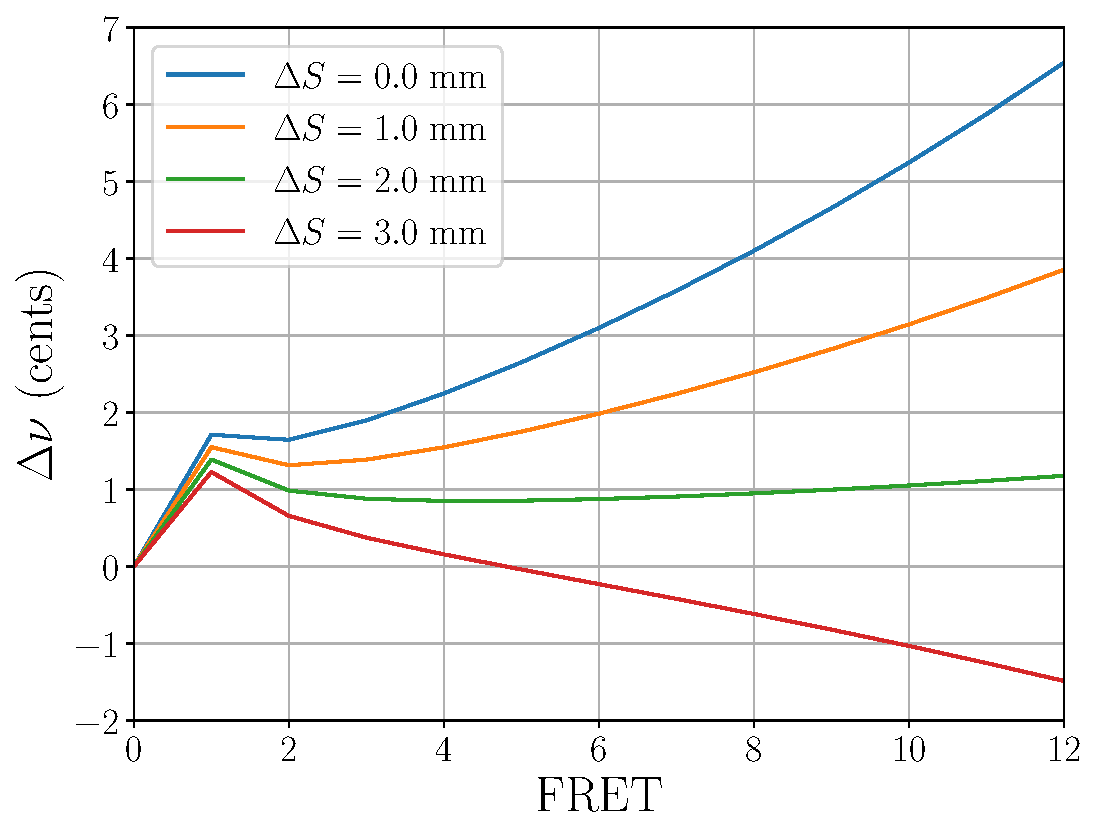
\includegraphics[width=5.0in]{../figures/comp_ds}
        \caption{Frequency shifts ($\Delta N = 0$)}
        \label{fig:comp_ds}
    \end{subfigure}
    \par\vspace{0.25in}
    \begin{subfigure}[b]{0.8\textwidth}
        \centering
        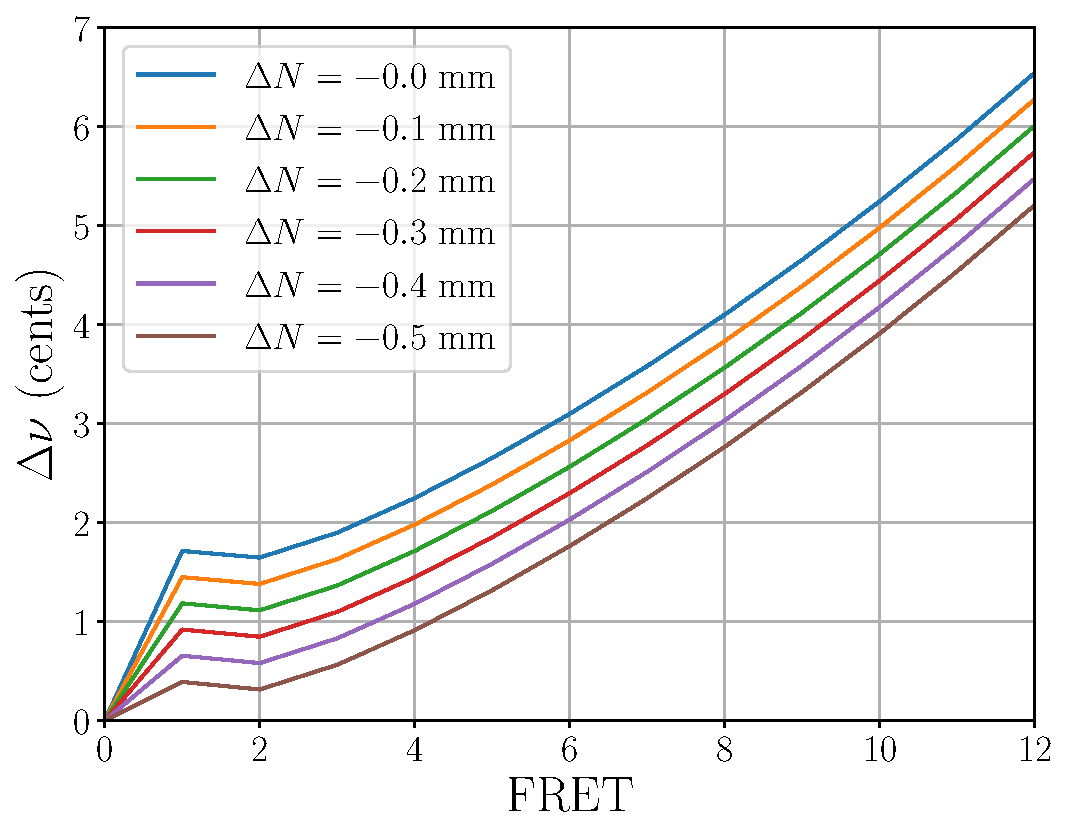
\includegraphics[width=5.0in]{../figures/comp_dn}
        \caption{Frequency shifts ($\Delta S = 0$)}
        \label{fig:comp_dn}
    \end{subfigure}
    \caption{\label{fig:comp_dsdn} In (a), we plot the frequency shifts for our classical guitar for several saddle setbacks with $\Delta N = 0$. Here $R = 24$ and the string radius is 0.5~mm. In (b), we set $\Delta S = 0$ and plot the frequency shifts for several nut ``setbacks.''}
  \end{figure}
  
  % \begin{figure}
  %   \centering
  %   \begin{subfigure}[b]{0.8\textwidth}
  %       \centering
  %       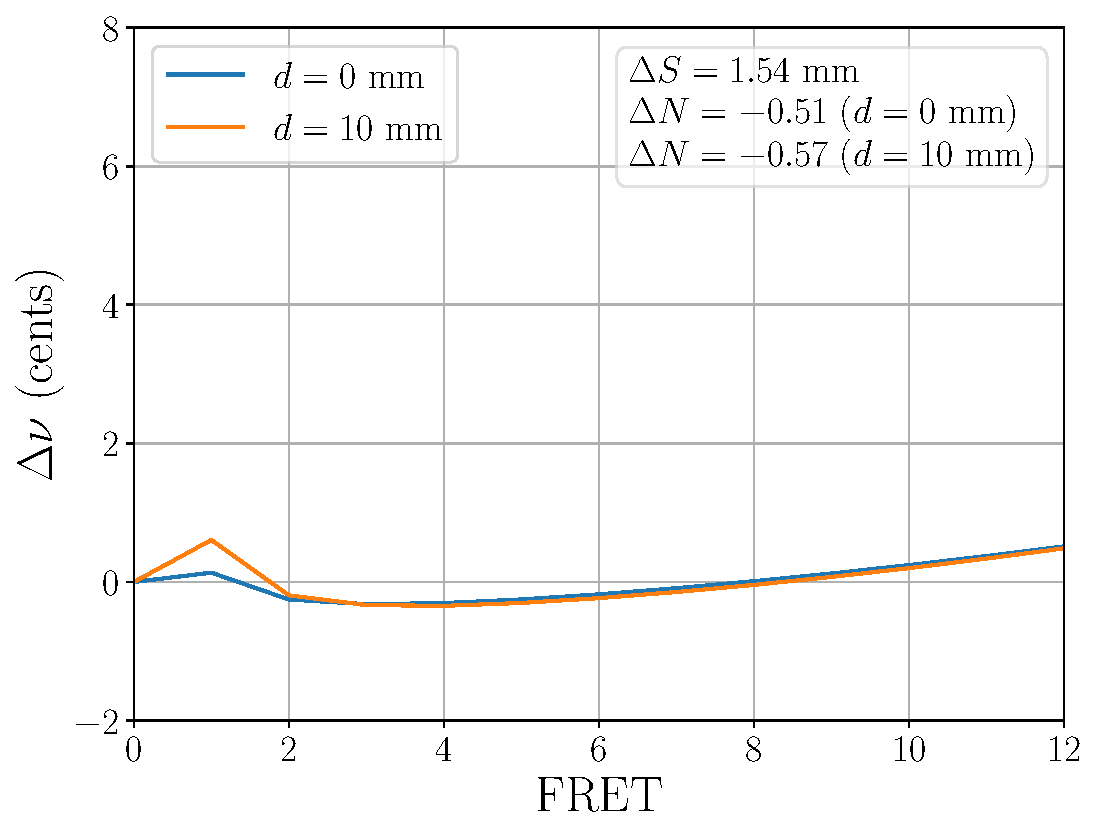
\includegraphics[width=5.0in]{../figures/comp_est}
  %       \caption{Approximate compensation}
  %       \label{fig:comp_est}
  %   \end{subfigure}
  %   \par\vspace{0.25in}
  %   \begin{subfigure}[b]{0.8\textwidth}
  %       \centering
  %       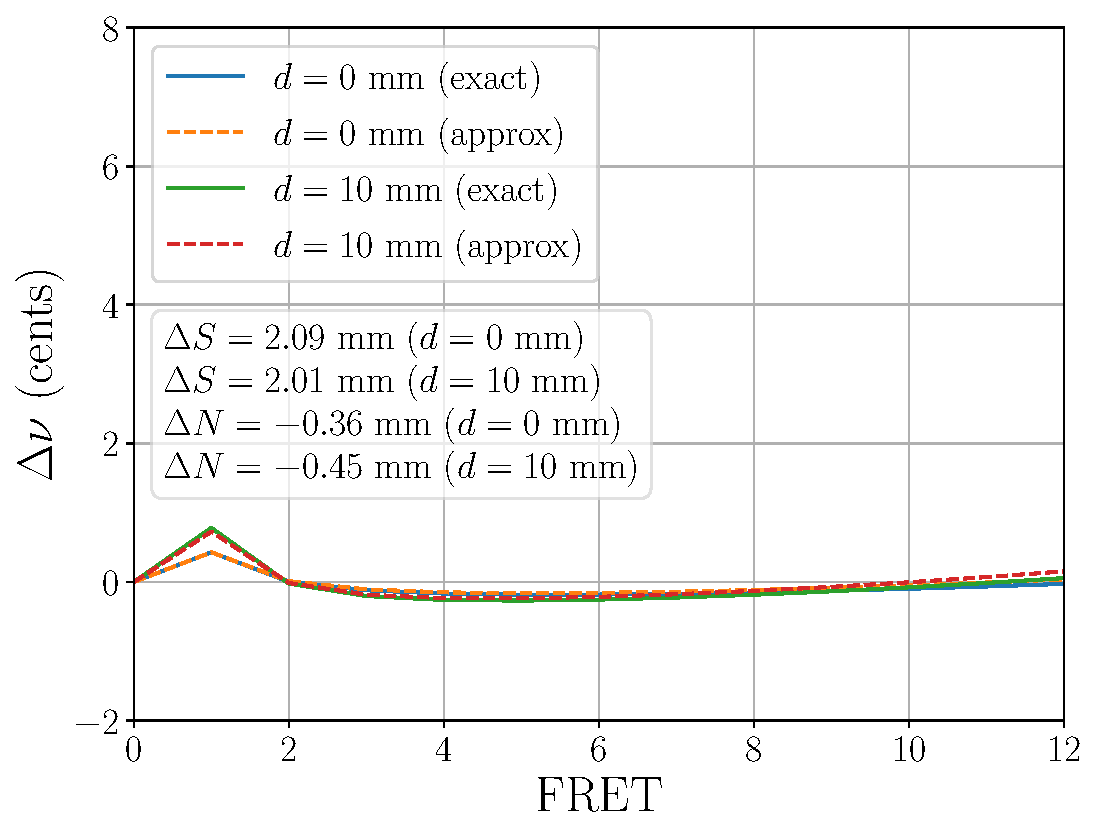
\includegraphics[width=5.0in]{../figures/comp_exact}
  %       \caption{Exact compensation}
  %       \label{fig:comp_exact}
  %   \end{subfigure}
  %   \caption{\label{fig:comp_model} In (a), we plot the frequency shifts for our classical guitar with approximate setbacks computed using \eqn{comp_approx}. In (b), we compute the same setbacks }
  % \end{figure}

\begin{figure}
  \centering
  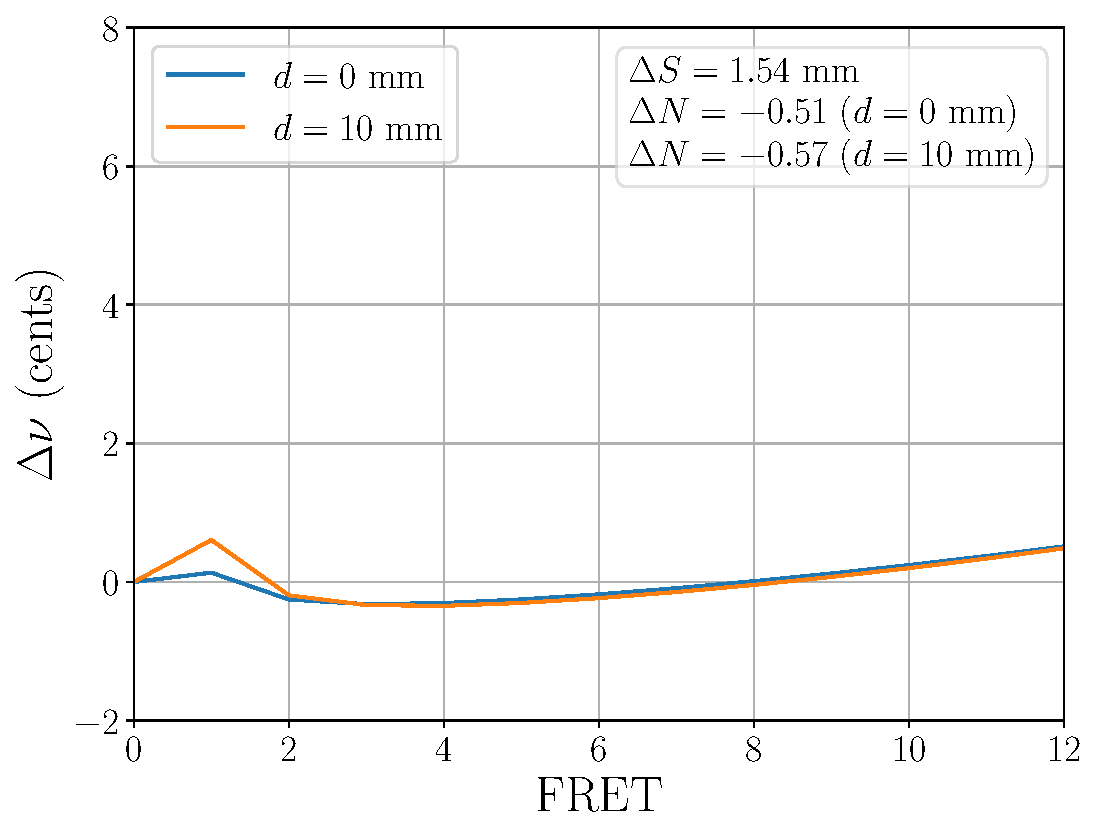
\includegraphics[width=5.0in]{../figures/comp_est}
  \caption{\label{fig:comp_est} The total frequency shift given by \eqn{error_def} for a classical guitar with a scale length of 650~mm, $b = 1.0$~mm, $c = 4.0$~mm, and a string with $R = 24$ and a radius $\rho = 0.5$~mm.}
\end{figure}

% Using the data and results presented in \tbl{ej45_props}, we can explore different approaches to compensating guitar strings for bending stiffness and string tension perturbations. For example, consider the guitar string shown in 

% For example, in \fig{shift_classicalguitar_ej45_factory}, using \eqn{error_def} we plot the frequency deviation (in cents) from ideal 12-TET for each string at each of the first 12 frets of an Alhambra 8P classical guitar, assuming that the open string has been perfectly tuned to the correct frequency. Recall that the Alhambra 8P is manufactured with a saddle setback of 1.5~mm, presumably to offset the effects of bending stiffness in the strings. For comparison, in \fig{shift_classicalguitar_ej45_null}, we plot the same deviations for the case where $\Delta S = 0$, which increases the error of each string at the 12$^\text{th}$ fret by 3 -- 4 cents. Recall from \sct{model} that we could crudely predict the values of the saddle and nut setbacks by inspecting \eqn{error_tot}. For example, from \tbl{ej45_props}, we estimate $\Delta S \approx B_0\, X_0 = 2.7$~mm and $\Delta N \approx -1.5$~mm for the third (G) string.

\begin{table}%[htbp]
  \centering
  \caption{\label{tbl:ej45_setbacks} Predicted setbacks for the D'Addario Pro-Arte Nylon Classical Guitar Strings -- Normal Tension (EJ45) on the Classical Guitar.}
  \begin{tabular}{cccc}
\toprule
String &  $\Delta S$ (mm) &  $\Delta N$ (mm) &  $\overline{\Delta \nu}_\text{rms}$ (cents) \\
\midrule
 J4501 &             2.16 &            -0.43 &                                        0.18 \\
 J4502 &             1.92 &            -0.31 &                                        0.15 \\
 J4503 &             4.36 &            -0.82 &                                        0.31 \\
 J4504 &             1.30 &            -0.19 &                                        0.13 \\
 J4505 &             1.94 &            -0.28 &                                        0.15 \\
 J4506 &             2.62 &            -0.35 &                                        0.16 \\
\bottomrule
\end{tabular}


\end{table}%

As an alternative to this simple approach, we adopt the method described in \app{rms} to compensate the Classical Guitar with normal tension nylon strings for the frequency errors shown in \fig{shift_classicalguitar_ej45_null}. Using \eqn{rms_sol_quad}, the setbacks we obtain for $d = 0$~mm are listed in \tbl{ej45_setbacks}, and the corresponding frequency deviations --- obtained with the listed setback for \emph{each} string --- are shown in \fig{shift_classicalguitar_ej45_full} (assuming that all other aspects of the guitar remain unchanged). Of course, manufacturing a guitar with unique saddle and nut setbacks for each string (of a particular tension) can be challenging, so we also plot in \fig{shift_classicalguitar_ej45_mean} the shifts obtained by setting each of the values of $\Delta S$ and $\Delta N$ to the mean of the corresponding column in  \tbl{ej45_setbacks}. In both cases, the RMS error is significantly smaller than that of the uncompensated guitar shown in \fig{shift_classicalguitar_ej45_null}. Note that the saddle setbacks tend to be larger --- and the nut setbacks smaller --- than the simple estimates that we made above for a hypothetical thick string. This is easily understood by examining \eqn{error_tot}: the portion of $\Delta S$ that exceeds $B_0\, X_0$ scales with $\gamma_n - 1$, and helps to compensate for tension errors as $n$ increases.

%  \begin{figure}
%   \centering
%   \begin{subfigure}[b]{0.8\textwidth}
%    \centering
%    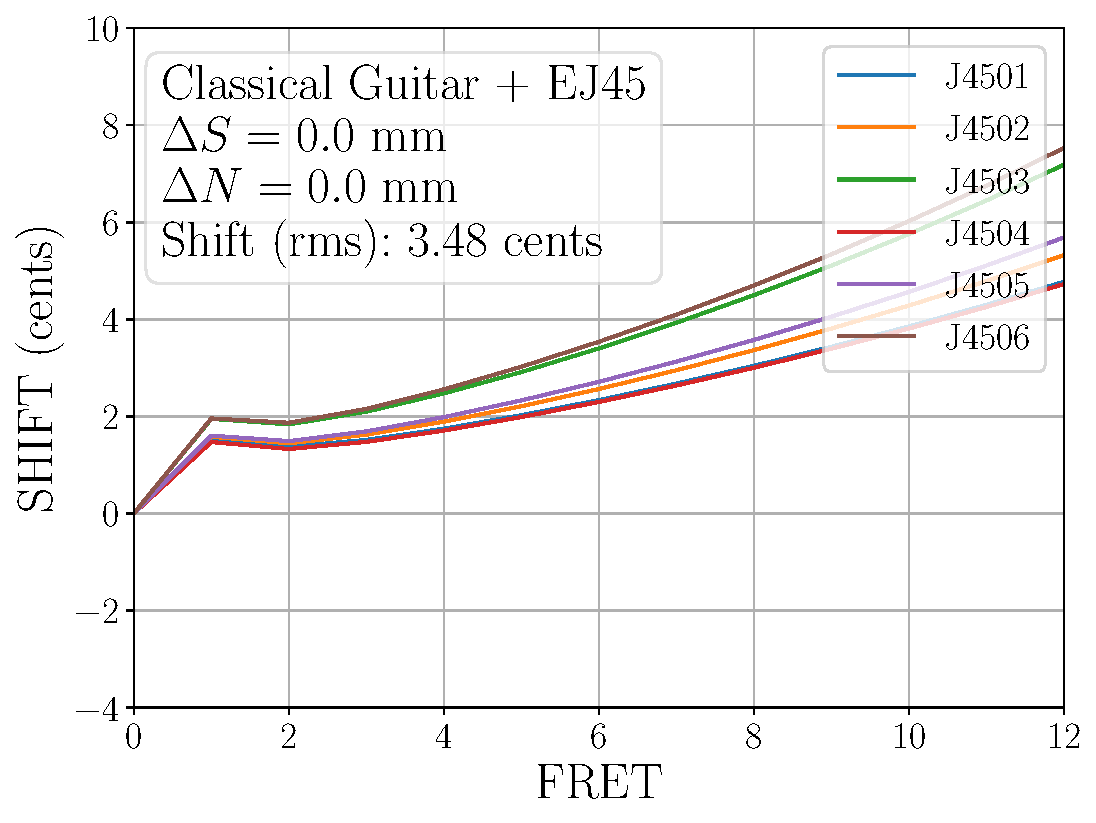
\includegraphics[width=5.0in]{../figures/shift_classicalguitar_ej45_factory}
%    \caption{Factory guitar}
%    \label{fig:shift_classicalguitar_ej45_factory}
%   \end{subfigure}
%   \par\vspace{0.25in}
%   \begin{subfigure}[b]{0.8\textwidth}
%    \centering
%    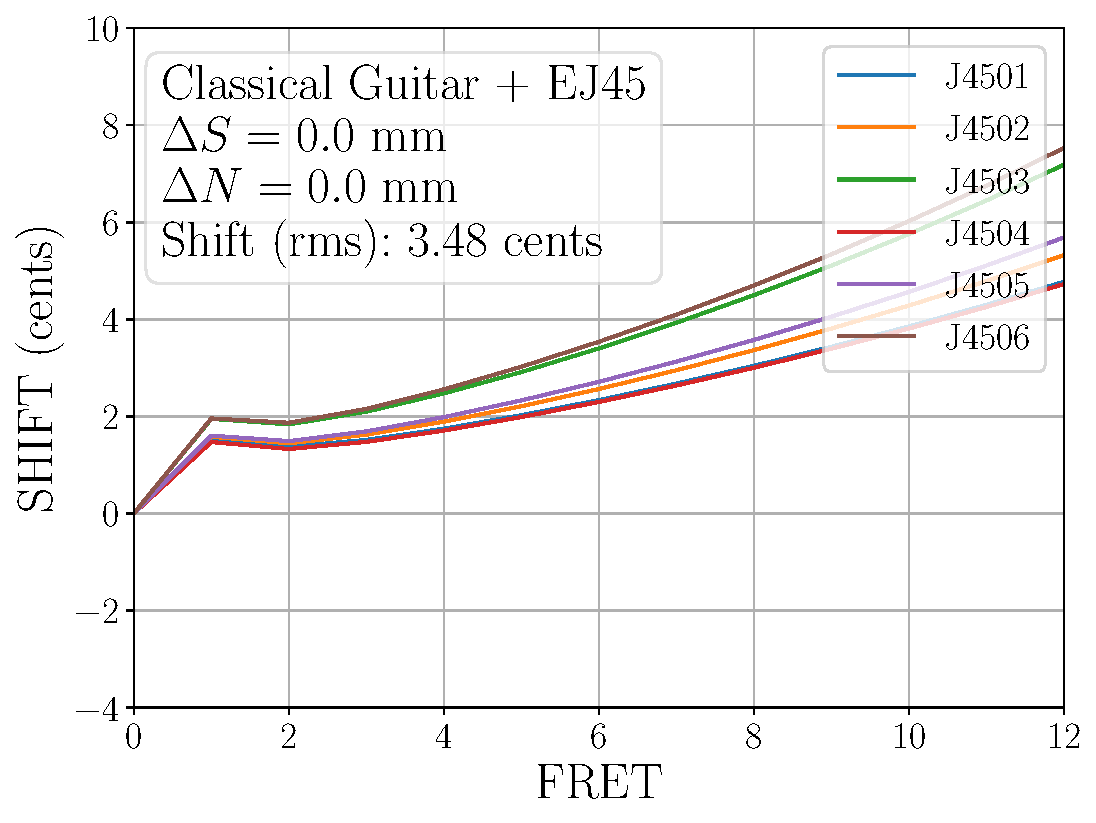
\includegraphics[width=5.0in]{../figures/shift_classicalguitar_ej45_null}
%    \caption{Uncompensated}
%    \label{fig:shift_classicalguitar_ej45_null}
%   \end{subfigure}
%   \caption{\label{fig:classicalguitar_ej45} Frequency shifts (in cents) for an Alhambra 8P guitar with normal tension nylon strings (D'Addario EJ45). In (a), we show the deviations of the guitar as manufactured in the factory, completely consistent with our measurements. In (b), we show the same 12-TET errors that would arise if $\Delta S = 0$ for the same guitar.}
%  \end{figure}

 \begin{figure}
  \centering
  \begin{subfigure}[b]{0.8\textwidth}
   \centering
   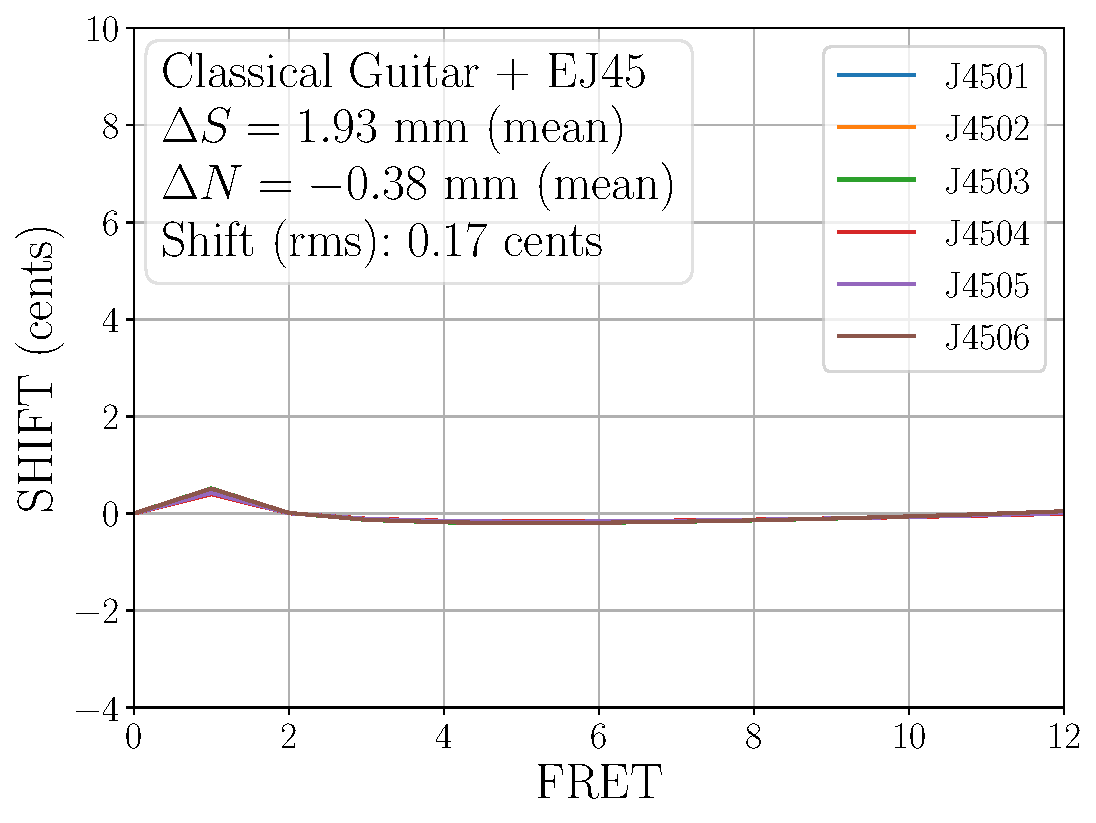
\includegraphics[width=5.0in]{../figures/shift_classicalguitar_ej45_full}
   \caption{Full compensation}
   \label{fig:shift_classicalguitar_ej45_full}
  \end{subfigure}
  \par\vspace{0.25in}
  \begin{subfigure}[b]{0.8\textwidth}
   \centering
   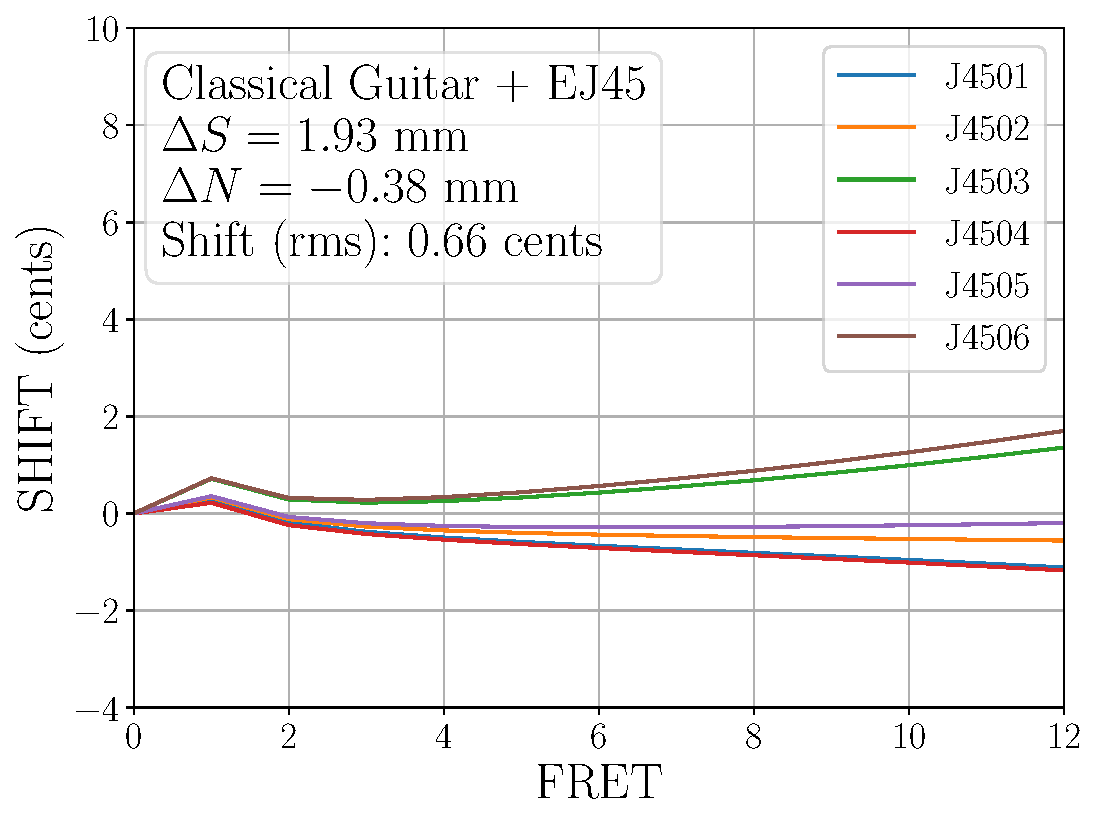
\includegraphics[width=5.0in]{../figures/shift_classicalguitar_ej45_mean}
   \caption{Mean compensation}
   \label{fig:shift_classicalguitar_ej45_mean}
  \end{subfigure}
  \caption{\label{fig:compensation_classicalguitar_ej45} Frequency shifts (in cents) for a classical guitar with normal tension nylon strings (D'Addario EJ45). In (a) we use the individual values for each string that are listed in \tbl{ej45_setbacks}. In (b), we set $\Delta S$ and $\Delta N$ to the mean of the corresponding column in that table.}
 \end{figure}

There are several other aspects of classical guitar compensation that are notable. First, as mentioned above, it is nontrivial to manufacture a guitar with different setbacks for each string~\cite{ref:byers1996cgi}, and it is unlikely that the exact values listed in \tbl{ej45_setbacks} are applicable to other string sets. We have measured the values of $R$ for five other string sets (with $d = 0$), and in \app{specs} we have reproduced the exact compensation procedure for them that we performed above for normal tension strings. Although each set exhibits variation between strings (and with respect to other sets) in individual setbacks for each string, they are similar enough that we suspect that there is the potential for great simplification in guitar design. For example, following the analysis of \app{rms}, it is possible to determine a single setback pair $\{\Delta S, \Delta N\}$ that minimizes the RMS frequency errors of an ensemble of strings over a collection of frets simply by computing the mean of the setbacks over all strings, and then using these mean values when manufacturing the guitar. If we consider five of the six string sets we have measured here --- neglecting the light tension strings because of their pathologically high values of $R$ --- 
we can plot the exact setback predictions shown in \fig{dsdn_mean}, and then use these results to predict the mean values. In \fig{fit_ds}, we see that the saddle setbacks are reasonably well described in terms of the string radius $\rho$ by the expression
\begin{equation}
  \Delta S = 4.41 \pm 0.24 \textrm{ mm}
\end{equation}
independent of the scale length. Therefore, we can either compute the mean of the saddle setbacks directly, or using the average value of the string lengths ($\overline{\rho} = 0.43$~mm). Either way, we obtain $\overline{\Delta S} = 1.9 \pm 0.1$~mm. Similarly, in \fig{hist_dn}, we show a histogram of the values of the nut setbacks, and compute the mean value $\Delta N = -0.38 \pm 0.04$~mm, which we recall is proportional to the scale length $X_0$. Note that these results are remarkably similar to the values used in \fig{shift_classicalguitar_ej45_mean}; if we plot the frequency deviations of those five string sets with these particular mean setback values, then we find that the maximum error always occurs at the twelfth fret, and it is always less than 1~cent. In the next section, we discuss a method to temper the guitar to reduce these errors further.

\begin{figure}
  \centering
  \begin{subfigure}[b]{0.8\textwidth}
   \centering
   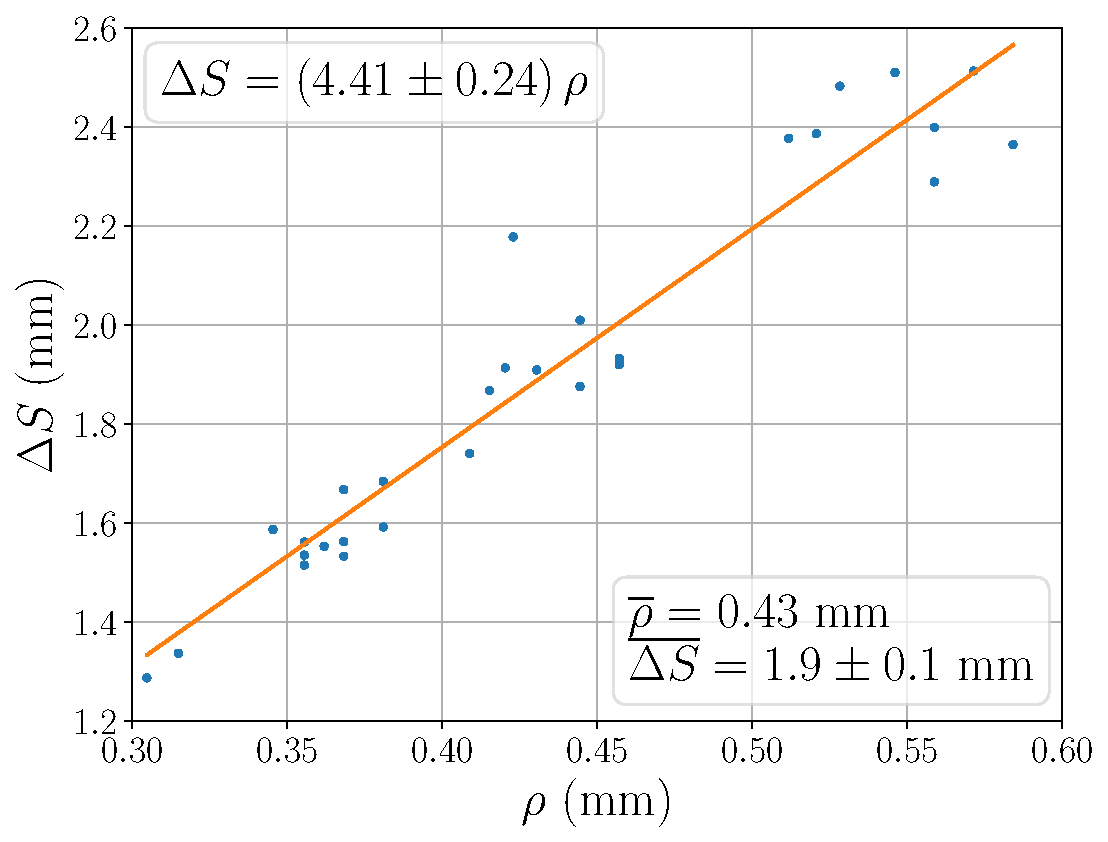
\includegraphics[width=5.0in]{../figures/fit_ds}
   \caption{Five-set saddle setback data with fit}
   \label{fig:fit_ds}
  \end{subfigure}
  \par\vspace{0.25in}
  \begin{subfigure}[b]{0.8\textwidth}
   \centering
   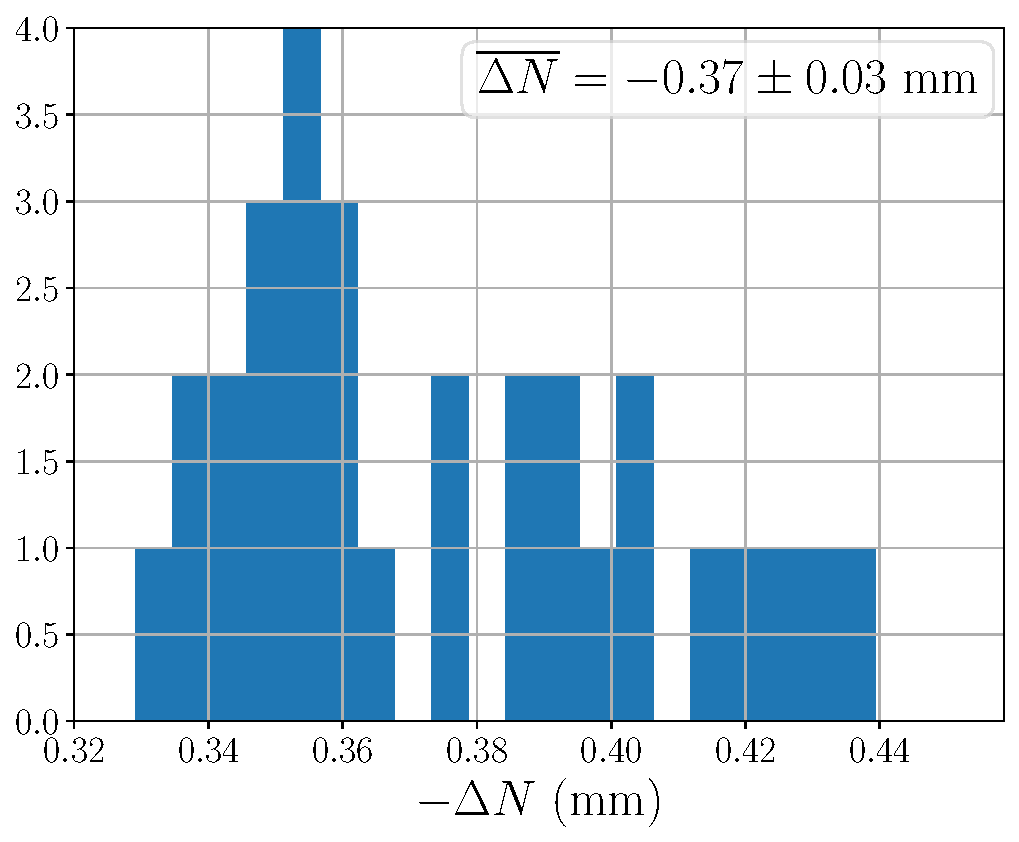
\includegraphics[width=5.0in]{../figures/hist_dn}
   \caption{Five-set nut setback data with mean}
   \label{fig:hist_dn}
  \end{subfigure}
  \caption{\label{fig:dsdn_mean} Construction of mean saddle and nut setbacks over five selected string sets. In (a) we plot the saddle setback for each string as a function of the string radius, with the result of the best linear fit. In (b), we present a histogram of the nut setbacks and their mean.}
 \end{figure}

Second, after paying close attention to the impact of the act of fretting on our approximations in \sct{model}, we have simply set $d = 0$ in this section. This is because nonzero values of $d$ have an impact on the frequency deviation of a string at the first fret, and are otherwise negligible. This tends to increase the required mean value of the nut setback, but does not require a significant change to the saddle setback. As an example, in \fig{dsdnd_ej45}, we plot the mean optimum saddle and nut setbacks for the classical guitar parameters used in \fig{shift_classicalguitar_ej45_mean} with the D'Addario Nylon Normal Tension EJ45 string set as a function of the fretting distance $d$. Paying careful attention to the $y$-axis of these plots, we see that the value of the mean saddle setback \emph{decreases} by less than 5\% as $d$ increases to 10~mm, and the magnitude of the nut setback increases by almost 30\% at the same fretting offset. This behavior is essentially the same for all string sets considered in this work, and can be used by the luthier to determine the optimum setback values for their designs. Note that --- when the RMS approach is used to compute the mean setbacks --- the difference $\Delta S - \Delta N$ (the sum of the saddle setback and the magnitude of the nut setback) is virtually independent of $d$, as shown in \fig{dsnd_ej45}. We see here that the distance between the saddle and the nut \emph{does not depend on} $d$; as $d$ increases, the saddle and the nut move together toward the guitar bridge at lower $x$ values. Therefore, for values of $b$ and $c$ that are within 50\% of those listed in \tbl{mcg_specs}, we can fit the change of $\Delta N$ to a polynomial in $d/X_0$, and find
\begin{align} \label{eqn:comp_d_poly}
  \Delta N(d) &\approx \Delta N(0) \left[ 1 + 13\, (d/X_0) + 280\, (d/X_0)^2 \right]\, , \nd \\
  \Delta S(d) &\approx \Delta S(0) + \Delta N(0) \left[13\, (d/X_0) + 280\, (d/X_0)^2 \right]\, .
\end{align}
As $d$ increases, the magnitude of the negative nut setback increases, and the saddle setback decreases because $\Delta N < 0$. Updating the guitar string illustrated in \fig{comp_est}, and using both \eqn{rms_sol_quad} with \emph{no} approximations (``exact'') and \eqn{rms_sol_comp} with \eqn{comp_d_poly} (``approx''), we find the setbacks and show the corresponding frequency deviations in \fig{comp_exact}. The setback values computed using these two methods are virtually identical.

\begin{figure}
  \centering
  \begin{subfigure}[b]{0.8\textwidth}
      \centering
      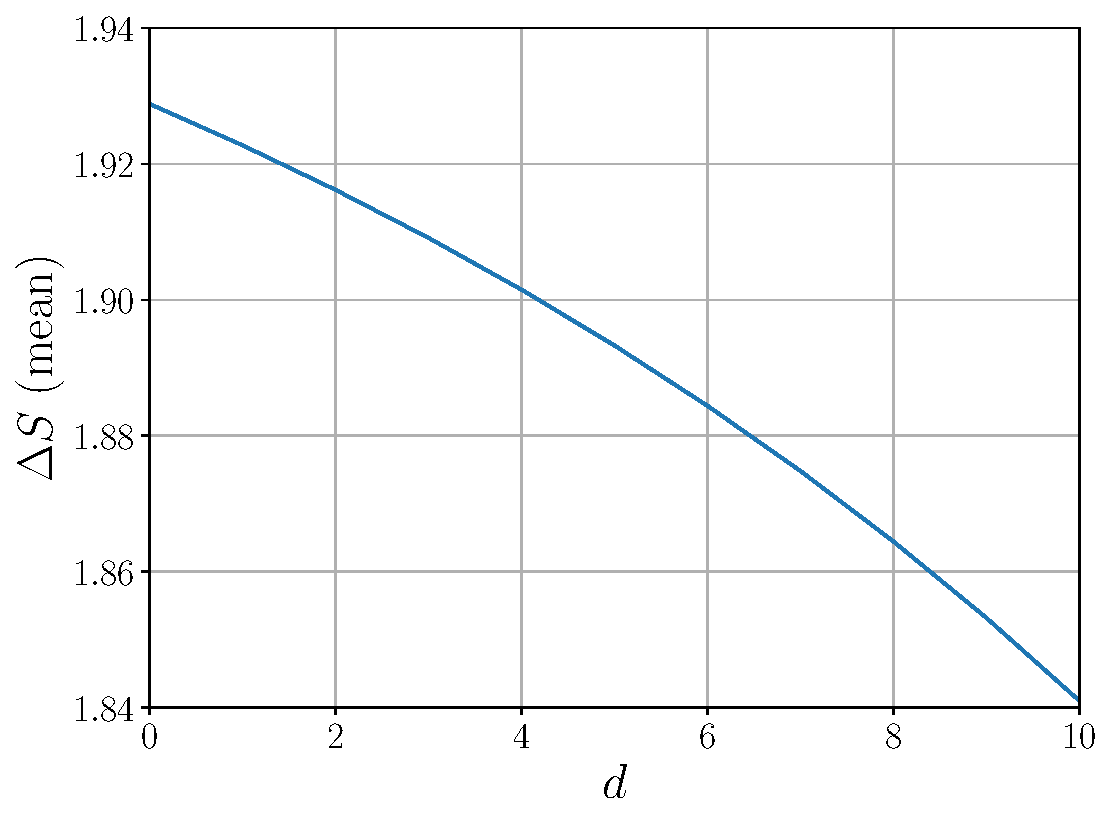
\includegraphics[width=5.0in]{../figures/dsd_ej45}
      \caption{Mean saddle setback}
      \label{fig:dsd_ej45}
  \end{subfigure}
  \par\vspace{0.25in}
  \begin{subfigure}[b]{0.8\textwidth}
      \centering
      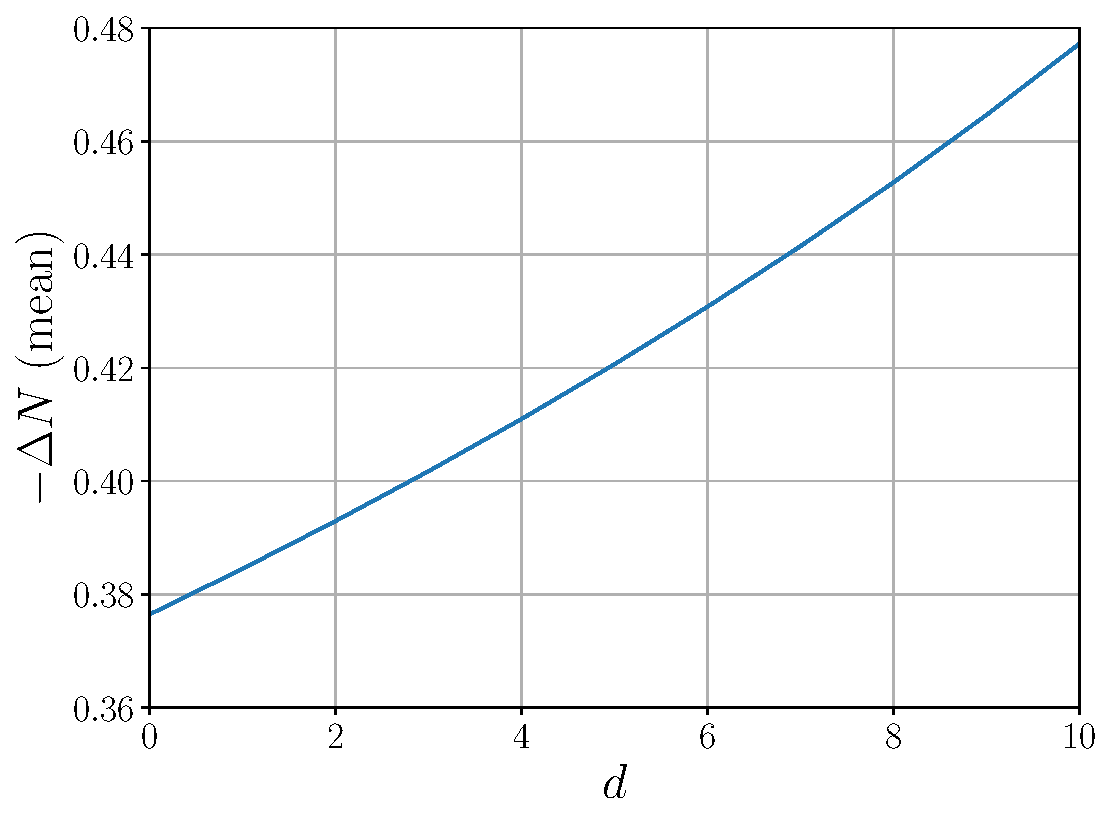
\includegraphics[width=5.0in]{../figures/dnd_ej45}
      \caption{Mean nut setback}
      \label{fig:dnd_ej45}
  \end{subfigure}
  \caption{\label{fig:dsdnd_ej45} The mean optimum saddle and nut setbacks for the D'Addario Nylon Normal Tension EJ45 string set as a function of the fretting distance $d$.}
\end{figure}

\begin{figure}
  \centering
  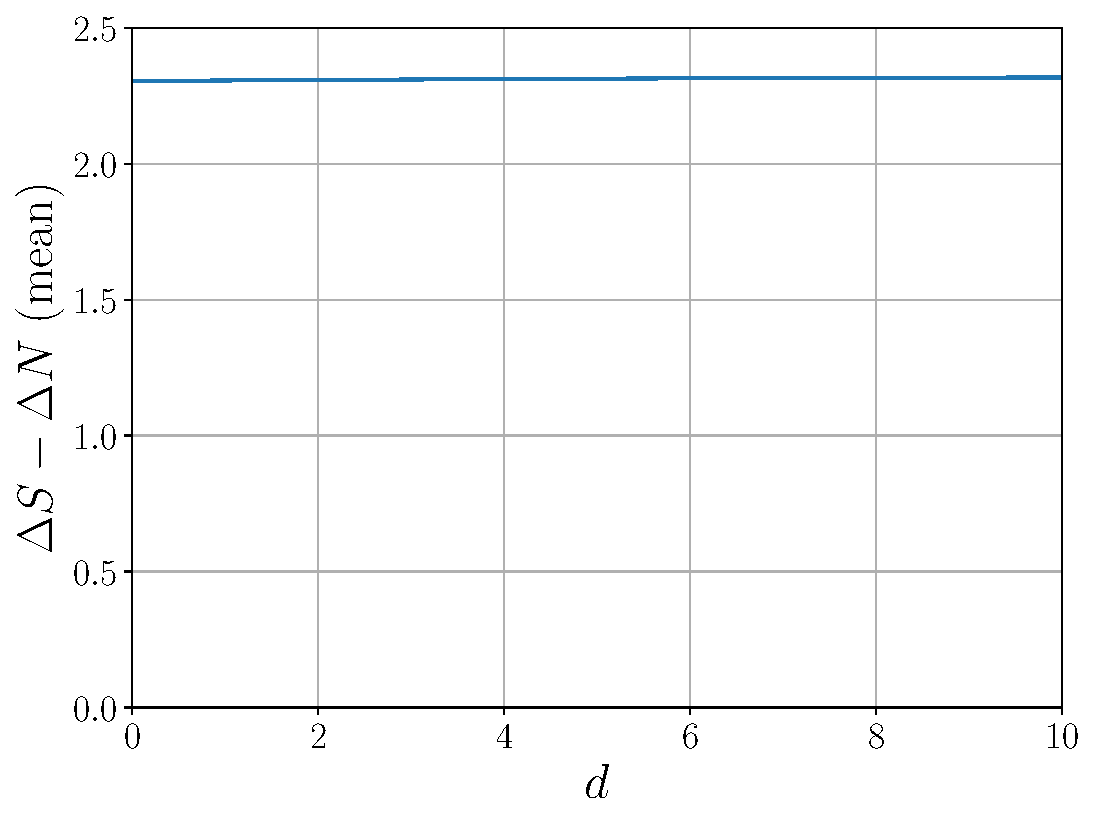
\includegraphics[width=5.0in]{../figures/dsnd_ej45}
  \caption{\label{fig:dsnd_ej45} The mean value of $\Delta S - \Delta N$ for the D'Addario Nylon Normal Tension EJ45 string set as a function of the fretting distance $d$.}
\end{figure}

\begin{figure}
  \centering
  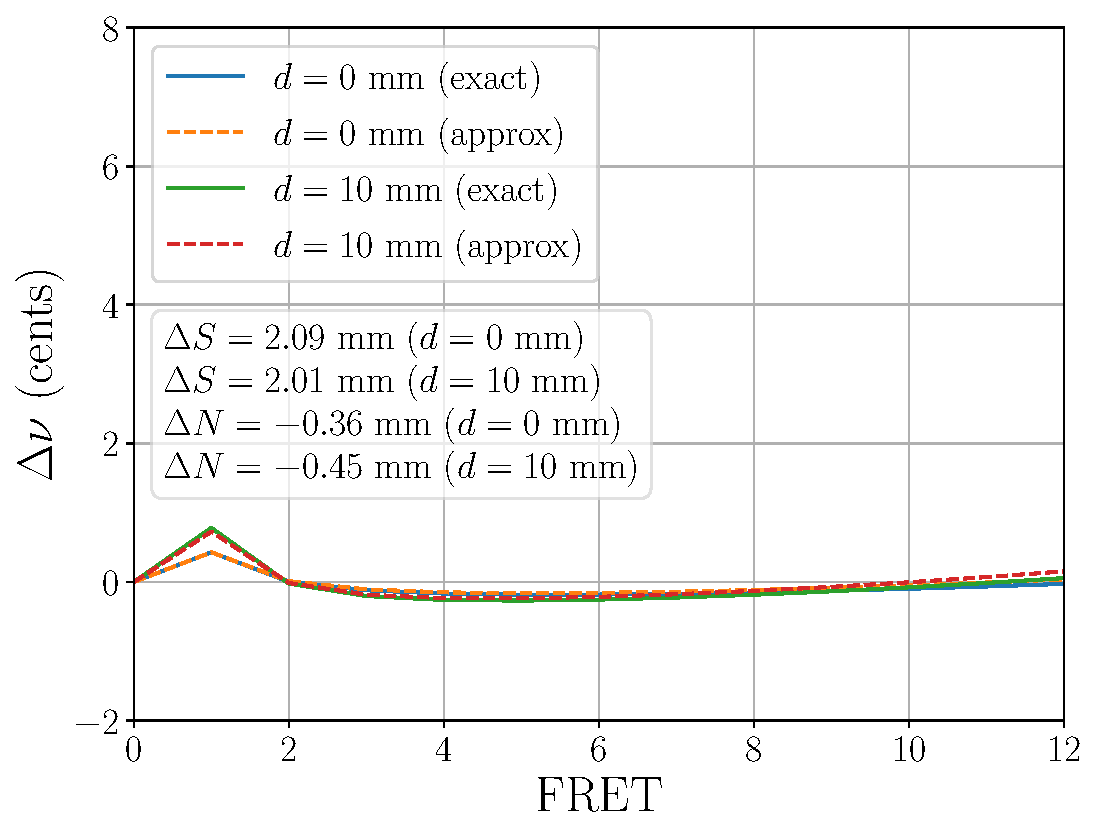
\includegraphics[width=5.0in]{../figures/comp_exact}
  \caption{\label{fig:comp_exact} The total frequency shift given by \eqn{error_def} for a classical guitar with setbacks computed using both \eqn{rms_sol_quad} with \emph{no} approximations (``exact'') and \eqn{rms_sol_comp} with \eqn{comp_d_poly} (``approx'').}
\end{figure}

\begin{figure}
  \centering
  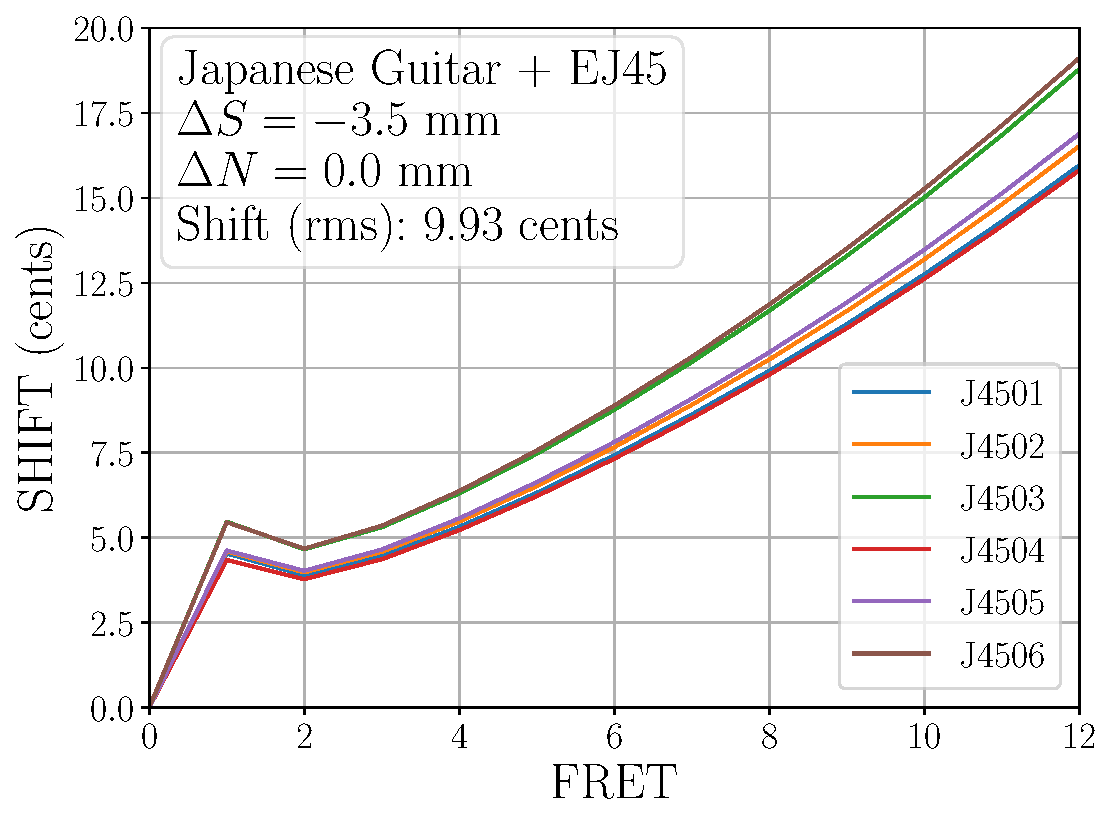
\includegraphics[width=5.0in]{../figures/japan_guitar_ej45_shifts}
  \caption{\label{fig:japan_guitar_ej45_shifts} Frequency shifts for a classical guitar using normal-tension nylon strings with $b = 1.4$~mm, $c = 5.5$~mm, $d = 10$~mm, $X_0 = 652$~mm, $\Delta S = -3.5$~mm, and $\Delta N = 0$~mm. The points represent the measurement data, while the lines are predictions made using \eqn{error_def}.}
\end{figure}

Third, recall that we recalculated the expected frequency shift of a classical guitar string with asymmetric boundary conditions in \app{freq}, and found an expression for $f_q$ given by \eqn{f_m_hybrid} that reduces --- by about a factor of 2 --- the impact of the bending stiffness relative to the symmetric (clamped) case in \eqn{f_m_clamped}. Furthermore, we have not used more sophisticated techniques to calculate the bending stiffness for either monofilament nylon strings or wound nylon strings, opting instead for the phenomenological model given by \eqn{b_0_kappa}. But is this approach valid? As a test, we compared our frequency shift estimates based on \sct{model} with experimental measurements made using a guitar manufactured in Japan with a few unique design choices: $b = 1.4$~mm, $c = 5.5$~mm, $d = 10$~mm, $X_0 = 652$~mm, $\Delta S = -3.5$~mm, and $\Delta N = 0$~mm. The larger value of $b$ and the large \emph{negative} saddle setback result in very large frequency deviations at all frets. As shown in \fig{japan_guitar_ej45_shifts}, we measured the shifts at the first fret and found that they fell into the range of $4.5 - 5.75$~cents, consistent with our predictions. At the 12$^\mathrm{th}$ fret, we measured $\Delta f = 18.5 - 19.5$~cents for the third and sixth strings, and $\Delta f = 15.75 - 17.5$~cents for the other strings, in reasonably close agreement with our predictions. By contrast, the corresponding equation arising from symmetric (clamped) boundary conditions --- \eqn{f_m_clamped} --- predicts shifts that are $30 - 45$\% higher, and setbacks that are more than a factor of two larger. We conclude that \eqn{f_m_hybrid} and \eqn{b_0_kappa} can be used to reliably predict setbacks for classical guitars.

Finally, many luthiers provide ``relief'' to enlarge the effective height of the string (particularly for the wound bass strings) as the fret number grows to provide clearance for vibration amplitude at higher volume. In practice, this is accomplished by pivoting the fret board shown in \fig{guitar_schematic} clockwise about $x = X_0$, increasing the height of the string above fret $n$ by an amount
\begin{equation}
  \begin{split}
    \Delta y_n &= m \left(X_0 - X_n\right) \\
    &= \frac{\gamma_n - 1}{\gamma_n}\, m\, X_0 \\
    &= \frac{\gamma_n - 1}{\gamma_n}\, 2\, \Delta y_{12}\, ,
  \end{split}
\end{equation}
where $\Delta y_{12}$ is the relief at the twelfth fret and $m = 2\, \Delta y_{12} / X_0 \ge 0$ is the downward slope of the fret board. If we update \eqn{l_n_def} and \eqn{l_p_def} (with $d = 0$), then we obtain
\begin{subequations}
  \begin{align}
    L_n &= \sqrt{\left(X_n + \Delta S\right)^2 + (b + \Delta y_n + c)^2}\, , \nd \\
    L^\prime_n &= \sqrt{\left(X_0 - X_n + \Delta N\right)^2 + \left(b + \Delta y_n\right)^2}\, .
  \end{align}
\end{subequations}
These equations indicate that we could update the approximation for $Q_n$ given by \eqn{q_n_approx} by replacing $b \longrightarrow b + \Delta y_n$, which results in the numerator
\begin{equation}
  \gamma_n\, b + (\gamma_n - 1)\, c \longrightarrow \gamma_n\, b + (\gamma_n - 1) \left(c + 2\, \Delta y_{12}\right)\, ,
\end{equation}
indicating that the intuitive substitution $c \longrightarrow c + 2\, \Delta y_{12}$ in \eqn{q_n_approx} captures the effect of relief. (Note that this should \emph{not} be done when computing the length $L_0$ of the open string!)

 %%%%%%%%%%%%%%%%%%%%%%%%%%%%%%%%%%%%%%%%%%%%%%%%%%%%%%%%%%%%%%%%%%%%%%%%%%%%%%
%
% Section file included in main project file using \input{}
%
% Assumes that LaTeX2e macros and packages defined in cg_comp.sty are
%   available
%
%%%%%%%%%%%%%%%%%%%%%%%%%%%%%%%%%%%%%%%%%%%%%%%%%%%%%%%%%%%%%%%%%%%%%%%%%%%%%%

 \section{Tempering the Classical Guitar\label{sct:temp}}

 \begin{quote}
 Temperament: A compromise between the acoustic purity of theoretically exact intervals, and the harmonic discrepancies arising from their practical employment. --- Dr.\ Theo.\ Baker~\cite{ref:baker1895dmt}
 \end{quote}

In \fig{shift_classicalguitar_ej45_mean}, a uniformly compensated classical guitar with normal tension strings tuned to 12-TET shows (of the treble strings) the third string has the greatest error in tuning across the fretboard. Tuning this guitar to 12-TET exacts a perfect-fifth in the third string while playing a C major chord in first position. This results in the third string being too sharp for the other common chords of E major (G\#), A major, and D major (A), particularly when the guitar is played at a higher fret position. One way to reduce this error is by lowering the pitch of the third string below 12-TET with an electronic tuner. Another more comprehensive system is to tune all the strings harmonically to the fifth string, which lowers the third string by 7 cents as well as tempering the remaining strings.

In this particular case, the ``Harmonic Tuning Method'' can be followed using these steps:
 \begin{enumerate}
  \item Begin by tuning the fifth string to A$_2 = 110$~Hz, resulting in a fifth-fret harmonic of A$_4 = 440$~Hz. (This can also be tuned by ear using an A$_4$ tuning fork).
  \item Tune that harmonic to the seventh fret harmonic of the fourth string, which is also A$_4 = 440$~Hz.
  \item Tune the seventh fret harmonic on the fifth string (330~Hz, or 0.37~Hz sharper than 12-TET E$_4$) to the fifth-fret harmonic of the sixth string.
  \item The seventh fret harmonic on the fifth string can tune the remaining fretted strings: the ninth fret on the third string, the fifth fret on the second string, and the open first string.
 \end{enumerate}
 \begin{table}[htbp]
  \centering
  \caption{\label{tbl:harmonic_tuning} Harmonic tuning methodology based on A$_4$ and E$_4$. The asterisk indicates a harmonic with a null at the designated fret.}
    \begin{tabular}{cc}
    \toprule
    Reference String/Fret &  Target String/Fret \\
    \midrule
     A$^\ast$/5 (A$_4$) & D$^\ast$/7 \\
     A$^\ast$/7 (E$_4$) & E$^\ast$/5 \\
     A$^\ast$/7 (E$_4$) & G/9 \\
     A$^\ast$/7 (E$_4$) & B/5 \\
     A$^\ast$/7 (E$_4$) & E/0 \\
    \bottomrule
    \end{tabular}
 \end{table}%

 \begin{figure}
  \centering
  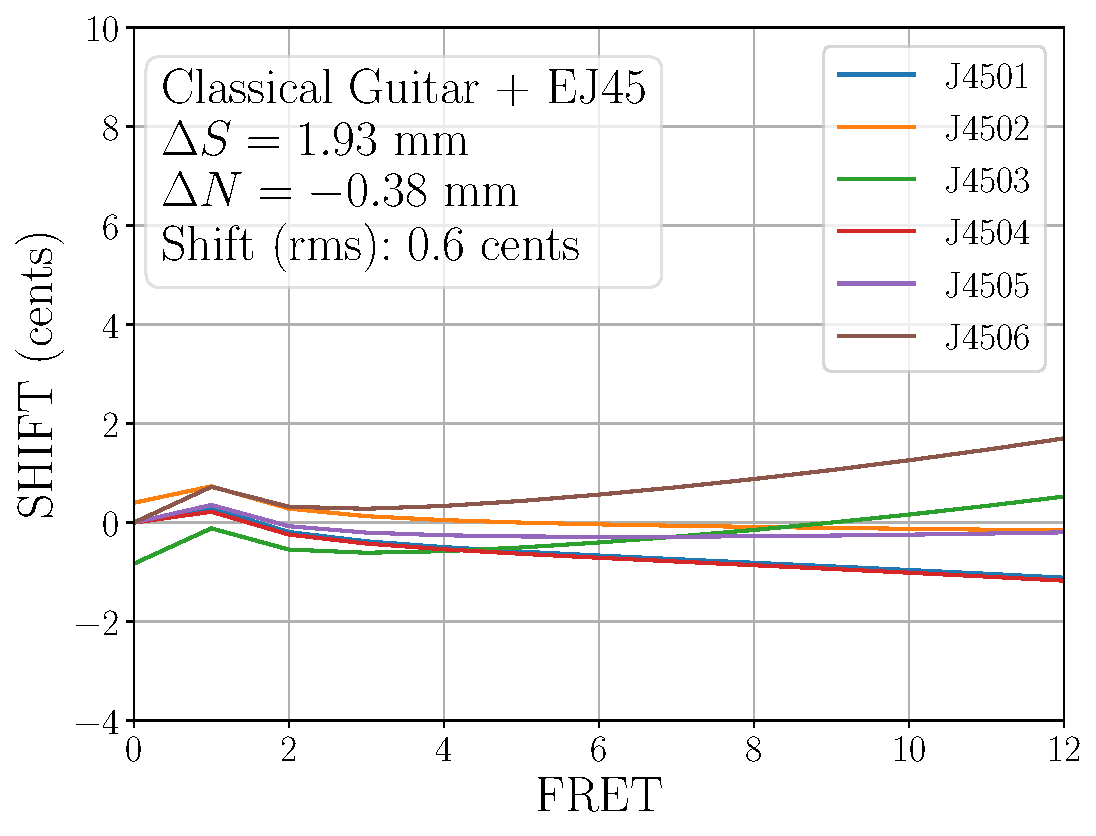
\includegraphics[width=5.0in]{../figures/shift_classicalguitar_ej45_harmonic}
  \caption{\label{fig:shift_classicalguitar_ej45_harmonic} Frequency shift (in cents) for the mean compensated classical guitar with normal tension nylon strings (D'Addario EJ45) shown with 12-TET tuning in \fig{shift_classicalguitar_ej45_mean}. Here the same guitar has been harmonically tuned using the approach outlined in \tbl{harmonic_tuning}.}
\end{figure}

 We have summarized these steps in \tbl{harmonic_tuning}, and in \fig{shift_classicalguitar_ej45_harmonic} we show the same guitar tuned in this fashion. Although the RMS shift over all strings is similar to that obtained by 12-TET tuning, the reduction in errors by strings 2 and 3 on the second and highewr frets is significant. Note that other tuning choices can be made depending on the piece being played. For example, the third string could also be tuned at the second fret to A$_3 = 220$~Hz using the fifth-string harmonic at the 12$^\text{th}$ fret, and/or the first string could be tuned at the fifth fret to A$_4$ using the fifth-fret harmonic of the fifth string. The flexibility of the harmonic tuning method --- and its reliance on only an A$_4$ tuning fork --- is a great asset for the classical guitarist.

% In fact, compensation at the factory and harmonic tuning can be combined to allow guitars with a wide variety of string sets to be well-tempered. For example, in \fig{shift_classicalguitar_ej45_comp_x3}, we plot frequency shifts (in cents) for an ``Alhambra 8P'' guitar with normal tension nylon strings (D'Addario EJ45). But, instead of the factory setbacks, we set $\Delta S$ and $\Delta N$ to the mean of the corresponding column in \tbl{ej45_setbacks} \emph{neglecting the third string}. This choice results in significant reductions in those setbacks, but the RMS frequency error for the third string is 4.7~cents for 12-TET tuning. In \fig{shift_classicalguitar_ej45_harm_x3}, we show that the harmonic tuning method described in \tbl{harmonic_tuning} reduces that RMS error to 2.2~cents.


%  \begin{figure}
%   \centering
%   \begin{subfigure}[b]{0.45\textwidth}
%    \centering
%    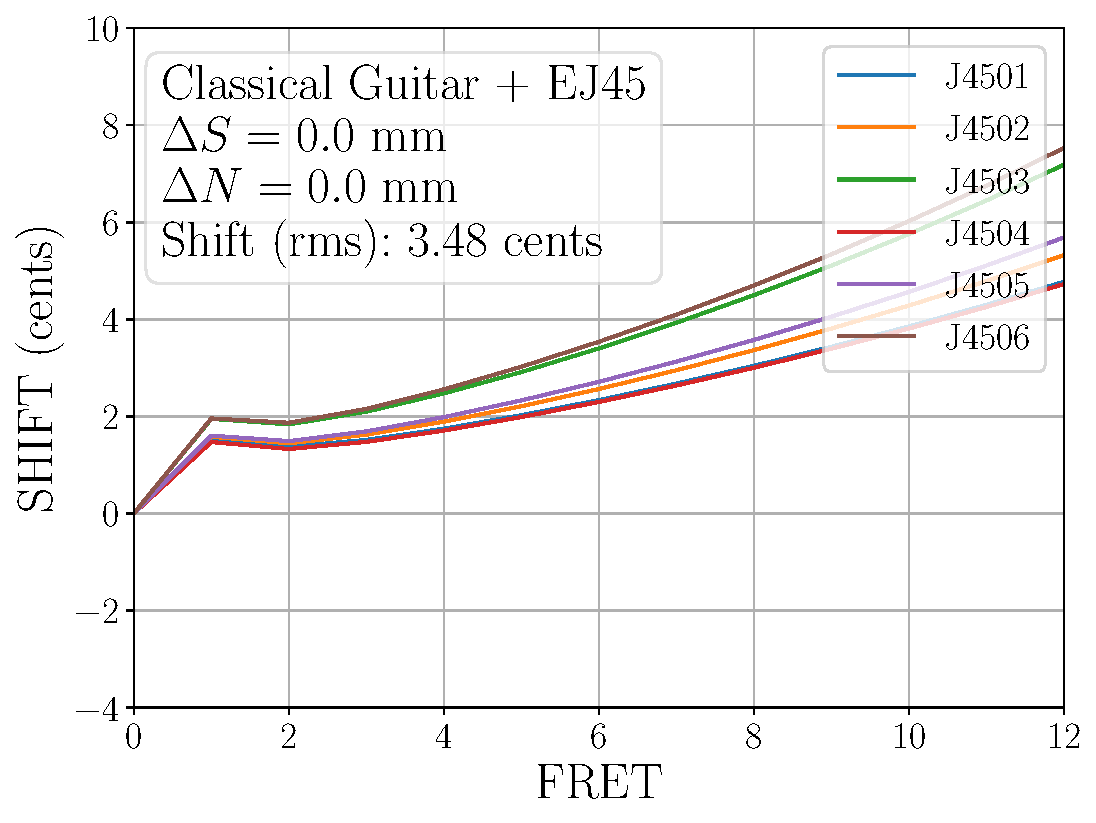
\includegraphics[width=3.25in]{../figures/shift_classicalguitar_ej45_factory}
%    \caption{Factory guitar --- 12-TET tuned}
%    \label{fig:shift_classicalguitar_ej45_fact_temp}
%   \end{subfigure}
%   \hspace{0.25in}
%   \begin{subfigure}[b]{0.45\textwidth}
%    \centering
%    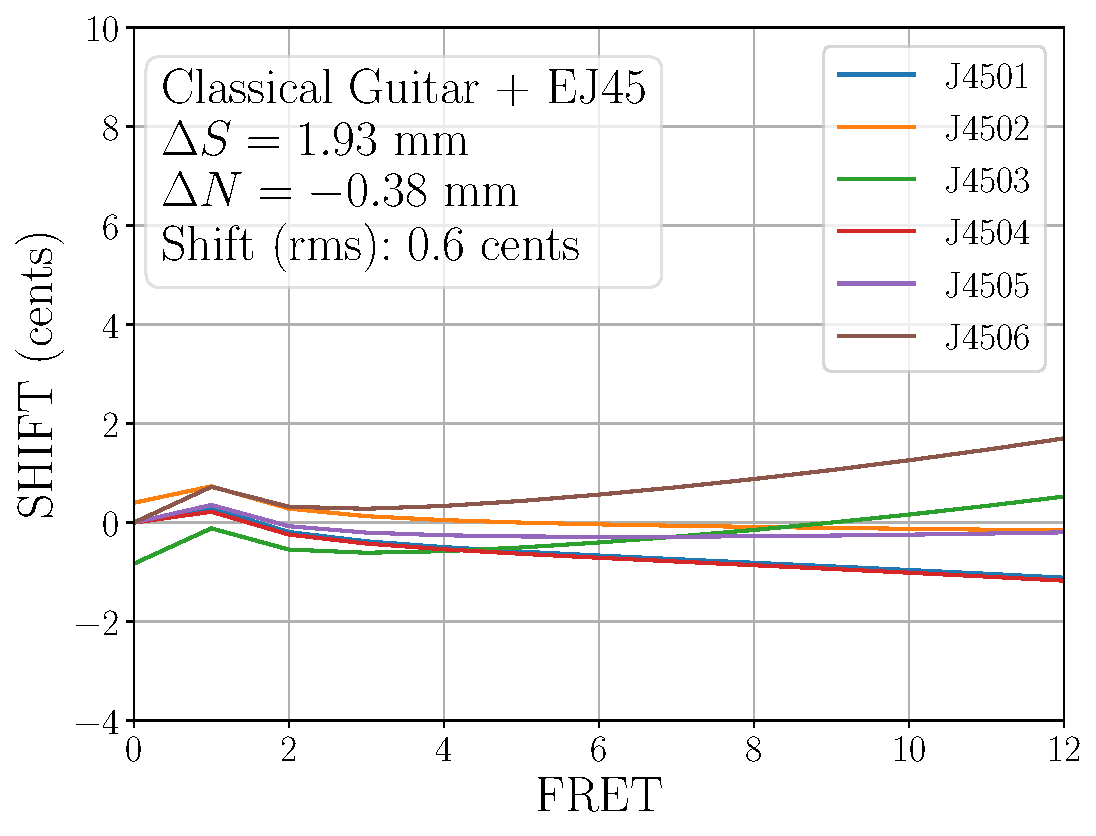
\includegraphics[width=3.25in]{../figures/shift_classicalguitar_ej45_harmonic}
%    \caption{Factory guitar --- harmonically tuned}
%    \label{fig:shift_classicalguitar_ej45_harmonic}
%   \end{subfigure}
%   \caption{\label{fig:compensation_classicalguitar_ej45_temp} Frequency shift (in cents) for an Alhambra 8P guitar with normal tension nylon strings (D'Addario EJ45). Here we compare (a) the factory guitar tuned to 12-TET with (b) the same guitar harmonically tuned using the approach outlined in \tbl{harmonic_tuning}.}
%  \end{figure}

%  \begin{figure}
%   \centering
%   \begin{subfigure}[b]{0.45\textwidth}
%    \centering
%    \includegraphics[width=3.25in]{../figures/shift_classicalguitar_ej45_comp_x3}
%    \caption{Compensated guitar --- 12-TET tuned}
%    \label{fig:shift_classicalguitar_ej45_comp_x3}
%   \end{subfigure}
%   \hspace{0.25in}
%   \begin{subfigure}[b]{0.45\textwidth}
%    \centering
%    \includegraphics[width=3.25in]{../figures/shift_classicalguitar_ej45_harm_x3}
%    \caption{Compensated guitar --- harmonically tuned}
%    \label{fig:shift_classicalguitar_ej45_harm_x3}
%   \end{subfigure}
%   \caption{\label{fig:compensation_classicalguitar_ej45_x3} Frequency shifts (in cents) for an ``Alhambra 8P'' guitar with normal tension nylon strings (D'Addario EJ45). Instead of the factory setbacks, in (a) we set $\Delta S$ and $\Delta N$ to the mean of the corresponding column in \tbl{ej45_setbacks} \emph{neglecting the third string}. In (b), we show the same guitar harmonically tuned using the approach outlined in \tbl{harmonic_tuning}.}
%  \end{figure}

 %%%%%%%%%%%%%%%%%%%%%%%%%%%%%%%%%%%%%%%%%%%%%%%%%%%%%%%%%%%%%%%%%%%%%%%%%%%%%%
%
% Section file included in main project file using \input{}
%
% Assumes that LaTeX2e macros and packages defined in cg_comp.sty are
%   available
%
%%%%%%%%%%%%%%%%%%%%%%%%%%%%%%%%%%%%%%%%%%%%%%%%%%%%%%%%%%%%%%%%%%%%%%%%%%%%%%

 \section{Conclusion\label{sct:conc}}

\begin{table}[htbp]
  \centering
  \caption{\label{tbl:ej45_ips} String properties for the D'Addario Pro-Arte Nylon Classical Guitar Strings -- Normal Tension (EJ45). The corresponding scale length is 25.5~inches.}
    \begin{tabular}{lcccc}
    \hline \hline
    String  & Note  & \multicolumn{1}{l}{Diameter (in)} & \multicolumn{1}{l}{Density (lb/in)} & \multicolumn{1}{l}{Tension (lb)} \\
    \hline
    J4501 & E$_4$  & 0.0280 & $2.092 \times 10^{-5}$ & 15.3 \\
    J4502 & B$_3$  & 0.0322 & $2.827 \times 10^{-5}$ & 11.6 \\
    J4503 & G$_3$  & 0.0403 & $4.679 \times 10^{-5}$ & 12.1 \\
    J4504 & D$_3$  & 0.0290 & $1.075 \times 10^{-4}$ & 15.6 \\
    J4505 & A$_2$  & 0.0350 & $1.842 \times 10^{-4}$ & 15.0 \\
    J4506 & E$_2$  & 0.0430 & $3.063 \times 10^{-4}$ & 14.0 \\
    \hline
    \end{tabular}%
  \label{tab:addlabel}%
\end{table}%

\begin{table}[htbp]
  \centering
  \caption{\label{tbl:ej45_mks} String properties for the D'Addario Pro-Arte Nylon Classical Guitar Strings -- Normal Tension (EJ45). The corresponding scale length is 650~mm.}
    \begin{tabular}{lcccc}
    \hline \hline
    String  & Note  & \multicolumn{1}{l}{Radius (mm)} & \multicolumn{1}{l}{Density (kg/mm)} & \multicolumn{1}{l}{Tension (N)} \\
    \hline
    J4501 & E$_4$  & 0.356 & $3.737 \times 10^{-7}$ & 68.6 \\
    J4502 & B$_3$  & 0.409 & $5.050 \times 10^{-7}$ & 52.0 \\
    J4503 & G$_3$  & 0.512 & $8.358 \times 10^{-7}$ & 54.3 \\
    J4504 & D$_3$  & 0.368 & $1.921 \times 10^{-6}$ & 70.0 \\
    J4505 & A$_2$  & 0.445 & $3.290 \times 10^{-6}$ & 67.3 \\
    J4506 & E$_2$  & 0.546 & $5.472 \times 10^{-6}$ & 62.8 \\
    \hline
    \end{tabular}%
  \label{tab:addlabel}%
\end{table}%

\begin{table}[htbp]
  \centering
  \caption{\label{tbl:ej43_ips} String properties for the D'Addario Pro-Arte Nylon Classical Guitar Strings -- Light Tension (EJ43). The corresponding scale length is 25.5~inches.}
    \begin{tabular}{lcccc}
    \hline \hline
    String  & Note  & \multicolumn{1}{l}{Diameter (in)} & \multicolumn{1}{l}{Density (lb/in)} & \multicolumn{1}{l}{Tension (lb)} \\
    \hline
    J4501 & E$_4$  & 0.0275 & $2.024 \times 10^{-5}$ & 14.8 \\
    J4502 & B$_3$  & 0.0317 & $2.729 \times 10^{-5}$ & 11.2 \\
    J4503 & G$_3$  & 0.0397 & $4.525 \times 10^{-5}$ & 11.7 \\
    J4504 & D$_3$  & 0.0280 & $1.020 \times 10^{-4}$ & 14.8 \\
    J4505 & A$_2$  & 0.0330 & $1.535 \times 10^{-4}$ & 12.5 \\
    J4506 & E$_2$  & 0.0420 & $2.888 \times 10^{-4}$ & 13.2 \\
    \hline
    \end{tabular}%
  \label{tab:addlabel}%
\end{table}%

\begin{table}[htbp]
  \centering
  \caption{\label{tbl:ej43_mks} String properties for the D'Addario Pro-Arte Nylon Classical Guitar Strings -- Light Tension (EJ43). The corresponding scale length is 650~mm.}
    \begin{tabular}{lcccc}
    \hline \hline
    String  & Note  & \multicolumn{1}{l}{Radius (mm)} & \multicolumn{1}{l}{Density (kg/mm)} & \multicolumn{1}{l}{Tension (N)} \\
    \hline
    J4501 & E$_4$  & 0.349 & $3.615 \times 10^{-7}$ & 66.4 \\
    J4502 & B$_3$  & 0.403 & $4.875 \times 10^{-7}$ & 50.2 \\
    J4503 & G$_3$  & 0.504 & $8.083 \times 10^{-7}$ & 52.5 \\
    J4504 & D$_3$  & 0.356 & $1.823 \times 10^{-6}$ & 66.4 \\
    J4505 & A$_2$  & 0.419 & $2.741 \times 10^{-6}$ & 56.1 \\
    J4506 & E$_2$  & 0.533 & $5.159 \times 10^{-6}$ & 59.2 \\
    \hline
    \end{tabular}%
  \label{tab:addlabel}%
\end{table}%




 \appendix
 %%%%%%%%%%%%%%%%%%%%%%%%%%%%%%%%%%%%%%%%%%%%%%%%%%%%%%%%%%%%%%%%%%%%%%%%%%%%%%
%
% Section file included in main project file using \input{}
%
% Assumes that LaTeX2e macros and packages defined in cg_comp.sty are
%   available
%
%%%%%%%%%%%%%%%%%%%%%%%%%%%%%%%%%%%%%%%%%%%%%%%%%%%%%%%%%%%%%%%%%%%%%%%%%%%%%%

 \section{Vibration Frequencies of a Stiff String\label{app:freq}}

Here we outline the calculation of the normal mode frequencies of a vibrating stiff string with non-symmetric boundary conditions. We begin with the wave equation~\cite{ref:fletcher1964nvf}
 \begin{equation}
\mu\, \frac{\partial^2}{\partial t^2}\, y(x) = T\, \frac{\partial^2}{\partial x^2}\, y(x) - E\, S\, \mathcal{K}^2\, \frac{\partial^4}{\partial x^2}\, y (x)\, ,
 \end{equation}
where $\mu$ and $T$ are respectively the linear mass density and the tension of the string, $E$ is its Young's modulus (or the modulus of elasticity), $S$ is the cross-sectional area, and $\mathcal{K}$ is the radius of gyration of the string. If we simplify this equation by scaling $x$ by the length $L$ of the string, and $t$ by $1/\omega_0 \equiv  (L/\pi) \sqrt{\mu/T}$, then we obtain the dimensionless wave equation
 \begin{equation} \label{eqn:wave_eqn_dim}
\pi^2\, \frac{\partial^2}{\partial t^2}\, y(x) = \frac{\partial^2}{\partial x^2}\, y(x) - B^2\, \frac{\partial^4}{\partial x^2}\, y (x)\, ,
 \end{equation}
where $B$ is the ``bending stiffness parameter'' given by
 \begin{equation} 
B \equiv \sqrt{\frac{E\, S\, \mathcal{K}^2}{L^2 T}}\, .
 \end{equation}
If we assume that $y(x)$ is a sum of terms of the form
 \begin{equation}
y(x) = \mathcal{C}\, e^{k\, x - i\, \omega\, t}\, ,
 \end{equation}
then $k$ and $\omega$ must satisfy the expression
 \begin{equation}
B^2 k^4 - k^2 - (\pi\, \omega)^2 = 0\, ,
 \end{equation}
or
 \begin{equation}
k^2 = \frac{1 \pm \sqrt{1 + (2\, \pi\, B\, \omega)^2}}{2\, B^2}\, .
 \end{equation}
Therefore, given $\omega$, we have four possible choices for $k$: $\pm k_1$, or $\pm i k_2$, where
 \begin{subequations} \label{eqn:disp_eqns}
 \begin{align}
\label{eqn:disp_eqn_1} k_1^2 &= \frac{\sqrt{1 + (2\, \pi\, B\, \omega)^2} + 1}{2\, B^2}\, , \nd \\
\label{eqn:disp_eqn_2} k_2^2 &= \frac{\sqrt{1 + (2\, \pi\, B\, \omega)^2} - 1}{2\, B^2}\, .
 \end{align}
 \end{subequations}
Therefore, the general solution to \eqn{wave_eqn_dim} has the form
 \begin{equation} \label{eqn:soln_dim}
y(x) = e^{-i \omega t} \left( C_1^+ e^{k_1 x} + C_1^- e^{-k_1 x} + C_2^+ e^{i k_2 x} + C_2^- e^{-i k_2 x} \right)\, .
 \end{equation}

As discussed in \sct{model}, the boundary conditions for the case of a classical guitar string are not symmetric. At $x = 0$ (the saddle), the string is pinned (but not clamped), so that $y = 0$ and $\partial^2 y/\partial x^2 = 0$. However, at $x = 1$ (the fret) the string is clamped, so that $y = 0$ and $\partial y/\partial x = 0$. Applying these boundary conditions to \eqn{soln_dim}, we obtain
 \begin{subequations}
 \begin{align}
  0 &= C_1^+ + C_1^- + C_2^+ + C_2^-\, , \\
  0 &= k_1^2 \left(C_1^+ + C_1^-\right) - k_2^2 \left(C_2^+ + C_2^-\right)\, , \\
  0 &= C_1^+ e^{k_1} + C_1^- e^{-k_1} + C_2^+ e^{i k_2} + C_2^- e^{-i k_2}\, , \nd \\
  0 &= k_1 \left(C_1^+ e^{k_1} - C_1^- e^{-k_1}\right) + i k_2 \left(C_2^+ e^{i k_2} - C_2^- e^{-i k_2}\right)\, .
 \end{align}
 \end{subequations}
Since $k_1^2 + k_2^2 \ne 0$, the first two of these equations tell us that $C_1^- = -C_1^+ \equiv -C_1$, and $C_2^- = -C_2^+ \equiv -C_2$. Therefore, the second two equations become
 \begin{subequations}
 \begin{align}
C_1\, \sinh(k_1) &= - i\, C_2\, \sin(k_2)\, , \nd \\
k_1\, C_1\, \cosh(k_1) &= -i\, k_2\, C_2\, \cos(k_2)\, .
 \end{align}
 \end{subequations}
Dividing the first of these equations by the second, we find
 \begin{equation}
\tan(k_2) = \frac{k_2}{k_1}\, \tanh{k_1}\, .
 \end{equation}

In the case of a classical guitar, we expect that $B \ll 1$, so from \eqn{disp_eqn_1} we see that $k_1 \approx 1/B \gg 1$, and therefore $\tanh{k_1} \longrightarrow 1$. Writing $k_2 = m \pi (1 + \epsilon)$, where $m$ is an integer greater than or equal to 1, and $\epsilon \ll 1$, we have $\tan(k_2) \approx m \pi \epsilon$, and
 \begin{equation}
\frac{k_2}{k_1} \approx m \pi B (1 + \epsilon) = m \pi \epsilon\, ,
 \end{equation}
indicating that $\epsilon = B$ to lowest order in $B$. To lowest (zero) order in $B$, we see from \eqn{disp_eqn_2} that $k_2 = \pi \omega = m \pi (1 + B)$, or $\omega = m (1 + B)$. Restoring the time scaling by $1/\omega_0$, and defining the frequency $f = \omega/2 \pi$, we finally have
 \begin{equation} \label{eqn:f_m_stiff}
f_m = \frac{m}{2\, L}\, \sqrt{\frac{T}{\mu}} (1 + B)\, .
 \end{equation}
We use this result to build our model in \sct{model}.
 %%%%%%%%%%%%%%%%%%%%%%%%%%%%%%%%%%%%%%%%%%%%%%%%%%%%%%%%%%%%%%%%%%%%%%%%%%%%%%
%
% Appendix file included in main project file using \input{}
%
% Assumes that LaTeX2e macros and packages defined in cg_comp.sty are
%   available
%
%%%%%%%%%%%%%%%%%%%%%%%%%%%%%%%%%%%%%%%%%%%%%%%%%%%%%%%%%%%%%%%%%%%%%%%%%%%%%%

 \section{Fretting Classical Guitar Strings\label{app:fret}}

\begin{figure}
    \centering
    \begin{subfigure}[b]{0.45\textwidth}
        \centering
        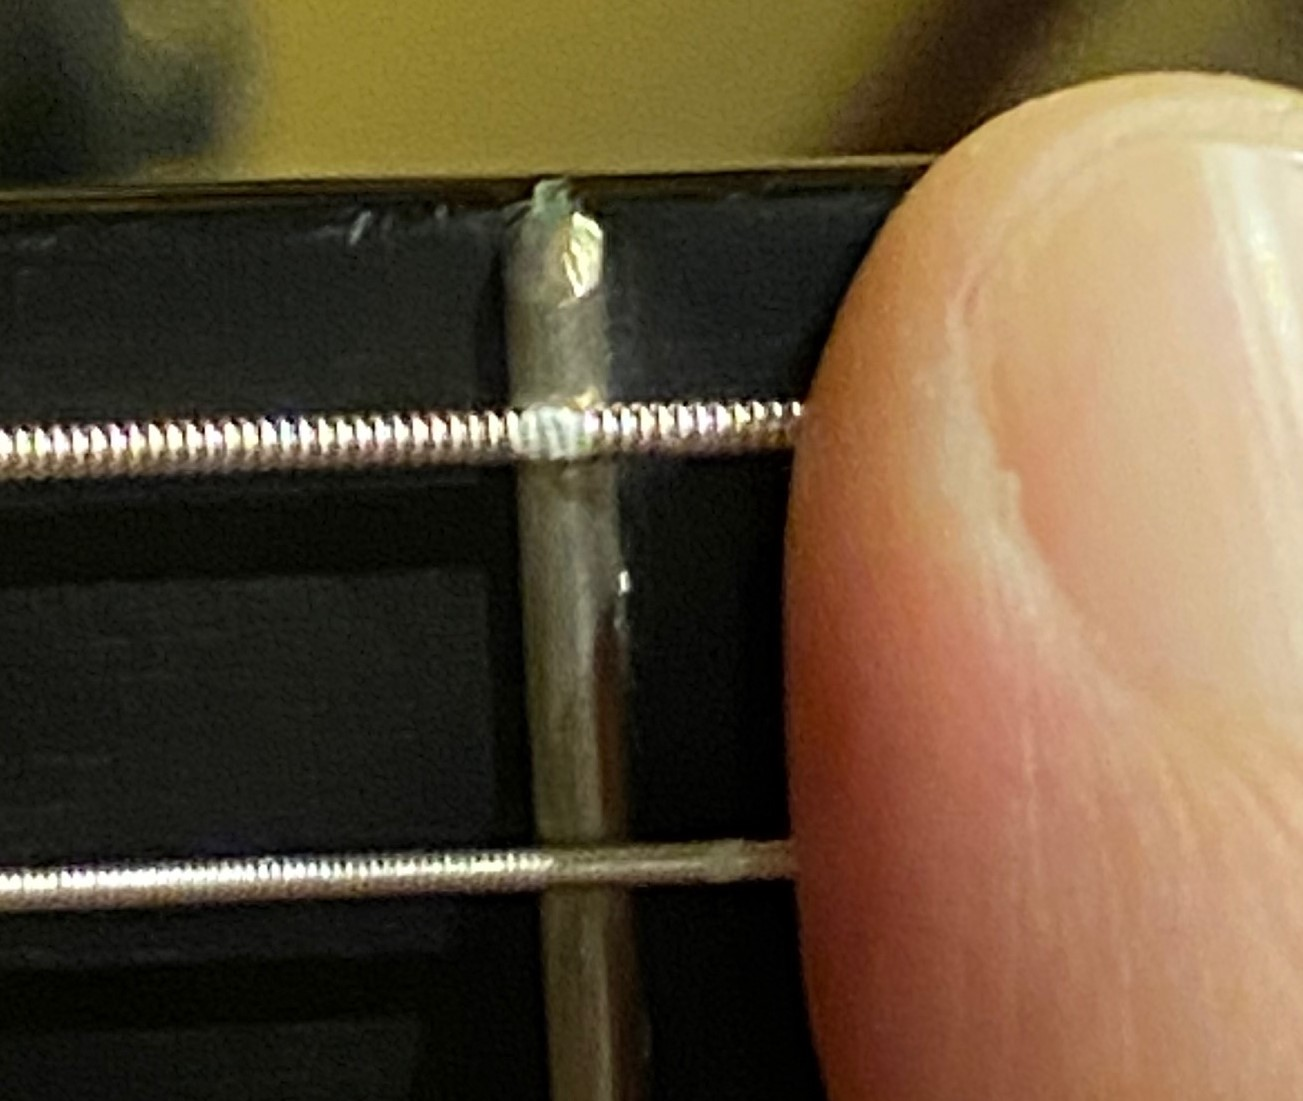
\includegraphics[width=3.0in]{../figures/fret_before.jpg}
        \caption{Before fretting}
        \label{fig:fret_before}
    \end{subfigure}
    \hspace{0.25in}
    \begin{subfigure}[b]{0.45\textwidth}
        \centering
        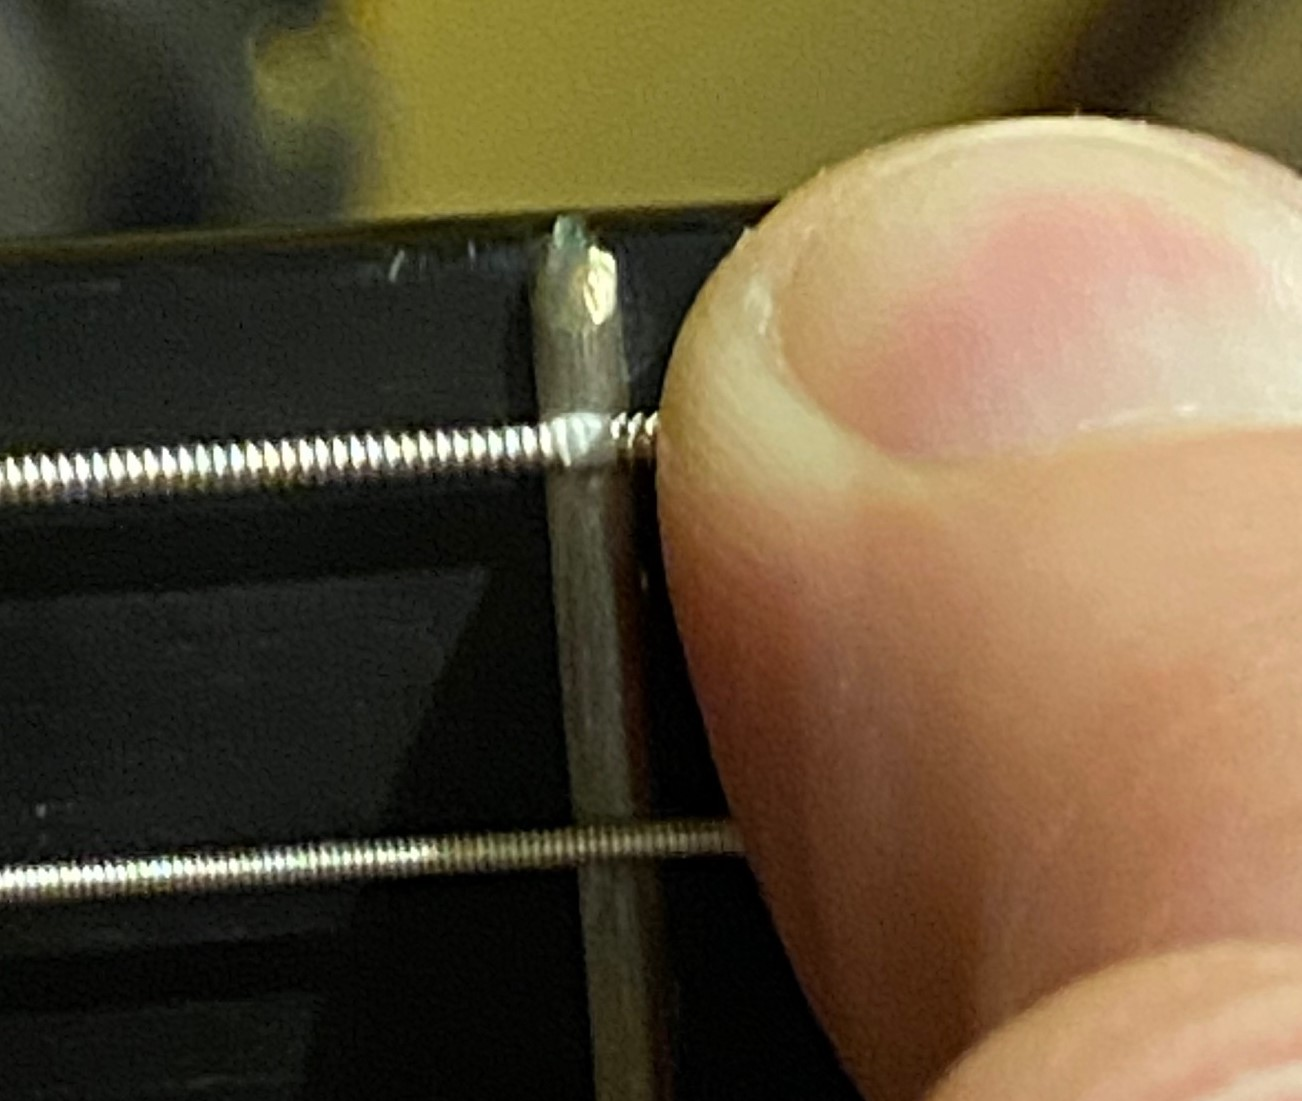
\includegraphics[width=3.04in]{../figures/fret_after.jpg}
        \caption{After fretting}
        \label{fig:fret_after}
    \end{subfigure}
    \caption{\label{fig:fret_befaft} Location of a small marker of white correction fluid before and after fretting.}
  \end{figure}
  
Previous studies of guitar intonation and compensation~\cite{ref:byers1996cgi,ref:varieschi2010icf} included a contribution to the incremental change in the length of the fretted string caused by both the depth and the shape of the string under the finger. As the string is initially pressed to the fret, the total length $\mathcal{L}_n$ increases and causes the tension in the string --- which is pinned at the saddle and clamped at the nut --- to increase. As the string is pressed further, does the additional deformation of the string increase its tension (throughout the resonant length $L_n$)? There are at least two purely empirical reasons to doubt this hypothesis. First, as shown in \fig{fret_befaft}, we can mark a string (with a small deposit of white correction fluid) above a particular fret and then observe the mark with a magnifying glass. As the string is pressed flat on the finger board with two fingers, the mark does not move perceptibly --- it has become \emph{clamped} on the fret. Second, we can use either our ears or a simple tool to measure frequencies~\cite{ref:pgtweb} to listen for a shift as we use different fingers and vary the fretted depth of a string. The apparent modulation is far less than would be obtained by classical vibrato ($\pm15$~cents), so we assume that once the string is minimally fretted the length(s) can be regarded as fixed. (If this were not the case, then fretting by different people or with different fingers, at a single string or with a barre, would cause additional, varying frequency shifts that would be audible and difficult to compensate.)


\begin{figure}
    \centering
    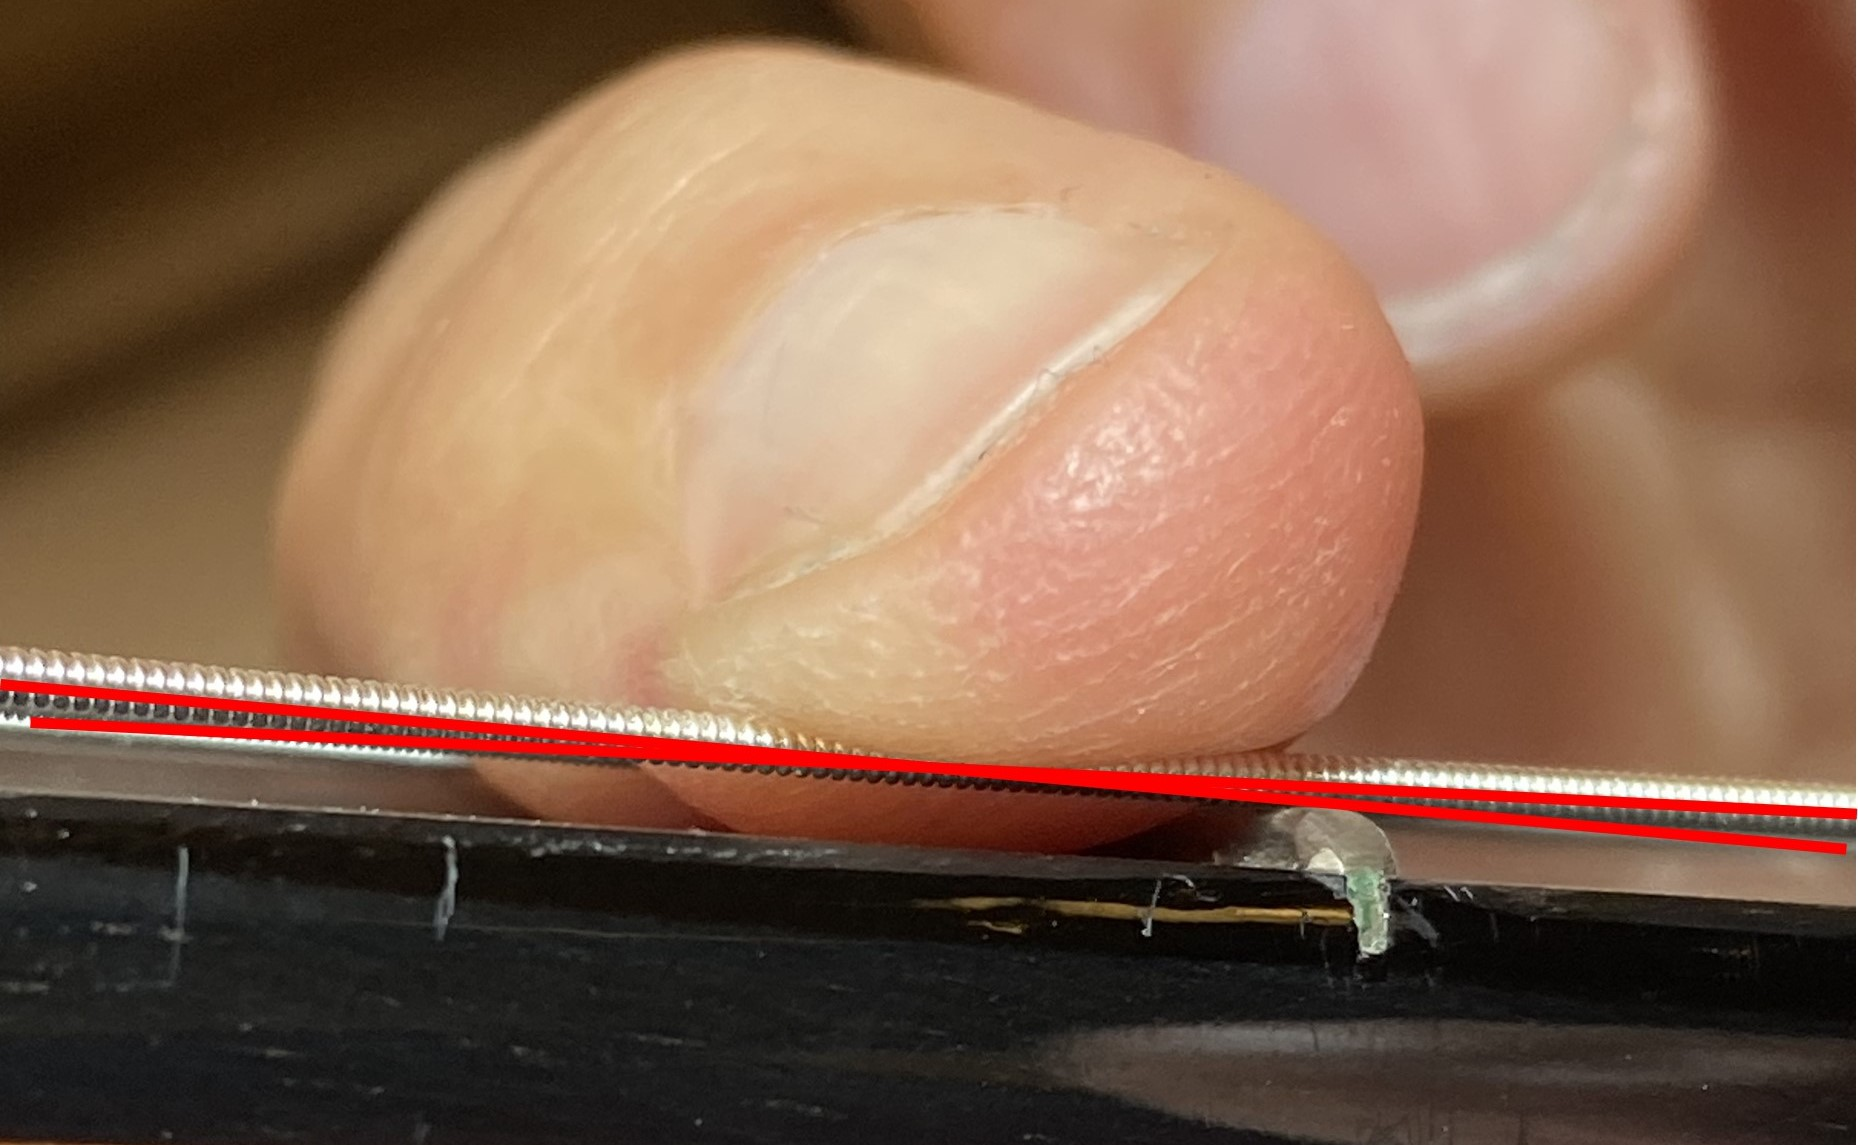
\includegraphics[width=6.0in]{../figures/fretting_photo}
    \caption{\label{fig:fretting_photo} Photo of a wound nylon $E_2$ string clamped at the first fret of a classical guitar. The shape of the fretted string can be well approximated by two line segments intersecting about 5--6~mm behind the fret.}
\end{figure}

% \begin{figure}
%     \centering
%     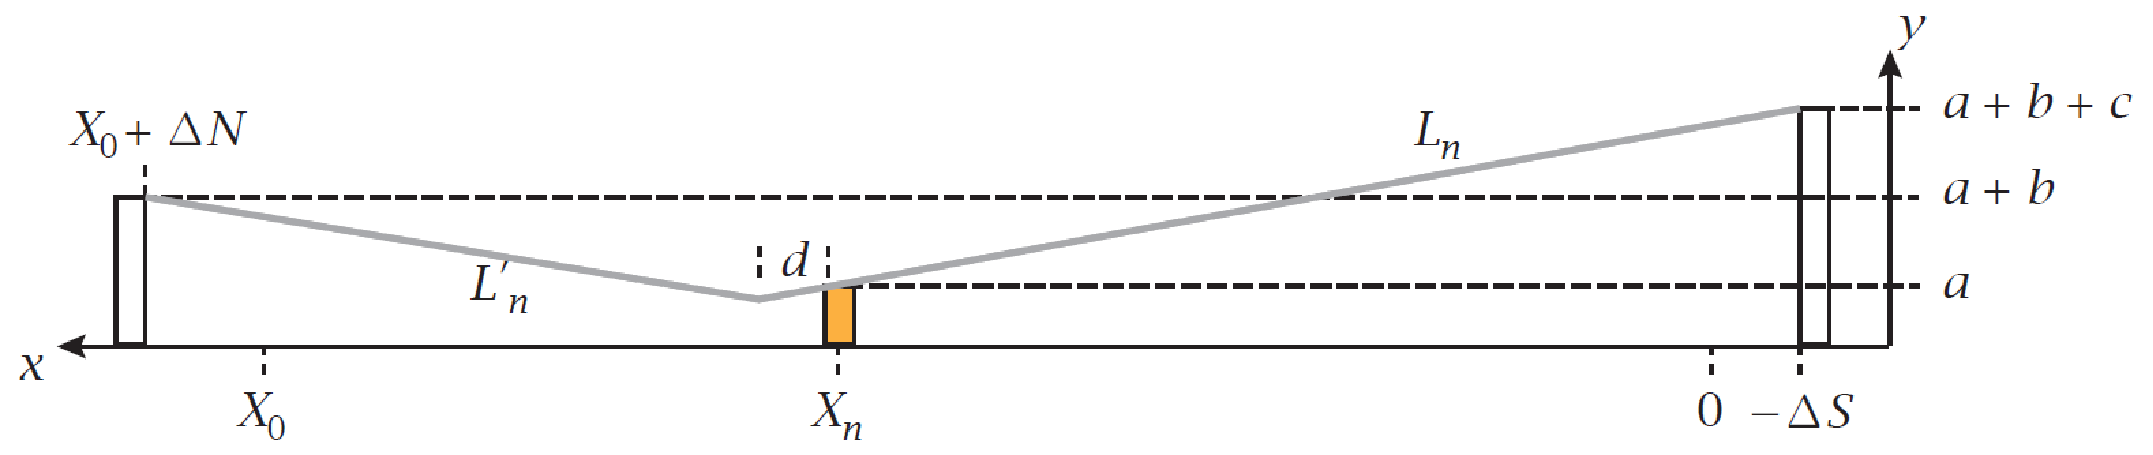
\includegraphics[width=6.0in]{../figures/fretting_schematic}
%     \caption{\label{fig:fretting_schematic} A recapitulation of \fig{guitar_schematic} with the addition of a line-segment intersection at a distance $d$ behind fret $n$ to represent the slight increase in the distance $L_n^\prime$ caused by a finger.}
% \end{figure}

In \sct{model}, we have included this concept in a simple way to determine the effect it will have on the frequency shift due to increased string tension. First, as shown in \fig{fretting_photo}, as the string is pressed onto the fret, its shape is described quite well by two line segments intersecting behind the fret. Here it is clear that the finger is shaped by the string more than the string is shaped by the finger. We have taken this observation into consideration in \fig{guitar_schematic} by introducing such an intersection point at a distance $d$ behind fret $n$ to represent the slight increase in the distance $L_n^\prime$ caused by a finger. The consequences of this choice are discussed in \sct{model_lmd}, and the impact it has on (for example) the relative displacement $Q_n$ is shown in \fig{qn_test}.


% In this case, the resonant length $L_n$ is unaffected, but after judicious use of similar triangles and the Pythagorean Theorem the remaining string length becomes
% \begin{equation}
%     \begin{split}
%         L^\prime_n &= \frac{L_n}{X_n + \Delta S}\, d + \sqrt{\left(X_0 - X_n + \Delta N - d\right)^2 + \left(b + \frac{b + c}{X_n + \Delta S}\, d\right)^2} \\
%         &\approx X_0 - X_n + \Delta N + \frac{b^2}{2 \left(X_0 - X_n\right)} + \frac{\left[(b + c)\, X_0 - c\, X_n\right]^2}{2 (X_0 - X_n)^2 X_n^2}\, d\, .
%     \end{split}
% \end{equation}
% The final term in this expression is smaller than the penultimate term by approximately $d/X_0$. We can use this result and \eqn{q_n_approx} to determine the increase in the relative displacement $Q_n$; we find
% \begin{equation} %\label{eqn:delta_q_n_approx}
%     \Delta Q_n \approx \left(\frac{\gamma_n}{\gamma_n - 1}\right)^2 \frac{b^2\, d}{2\, X_0^3}\, .
% \end{equation}
% \begin{equation} %\label{eqn:delta_q_n_approx}
%     \begin{split}
%         \Delta Q_n &\approx \frac{\gamma_n^2\, d}{2\, X_0^3} \left( \frac{\gamma_n}{\gamma_n - 1}\, b + c \right)^2 \\
%         &= Q_n\, \frac{\gamma_n^2}{\gamma_n - 1}\, \frac{d}{X_0}\, .
%     \end{split}
% \end{equation}
% Unless
% \begin{equation}
%     c > \left[ \frac{1}{(\gamma_{1} - 1) (\gamma_{12} - 1)} - 1 \right] b\, ,
% \end{equation}
% $\Delta Q_n$ is largest when $n = 1$. 

% The first factor on the \rhs of this expression is well approximated as
% \begin{equation}
%     \left(\frac{\gamma_n}{\gamma_n - 1}\right)^2 \approx \left[\frac{12}{n\, \ln(2)}\right]^2\, ,
% \end{equation}
% which is clearly largest at the first fret. When $d > 0$, the corresponding increase in the frequency shift given by \eqn{error_tot} is
% \begin{equation} \label{eqn:delta_nu_n_d}
%     \Delta \nu_n(d) - \Delta \nu_n(0) = \frac{600}{\ln(2)}\, \left(\frac{\gamma_n}{\gamma_n - 1}\right)^2 \frac{\kappa\, b^2\, d}{2\, X_0^3}\, .
% \end{equation}

% In \fig{fret_disp}, we plot $\Delta Q_1 / Q_1$ as a function of the distance parameter $d$. We see that a narrow finger ($d \approx 5$~mm) introduces a relative change in $Q_1$ --- and therefore a corresponding fractional increase in the frequency shift due to increases in tension --- of approximately 15\%. A large finger that is twice as wide results in a 30\% correction. 
% For a string with $\kappa = 49$, in \fig{fret_shift} we plot $\Delta \nu_n(d) - \Delta \nu_n(0)$ as a function of $d$. In this case, the shift for a finger with $d = 10$~mm is less than 0.5~cents. It is true that we can press the string so hard that it touches the fret board, but the increase in the frequency shift is still less than 1~cent, and this is likely the result of dragging the string over the fret (similar to vibrato) and causing a local change in tension that is inconsistent with the boundary conditions used to derive \eqn{f_m_stiff}.

% \begin{figure}
%     \centering
%     \begin{subfigure}[b]{0.8\textwidth}
%         \centering
%         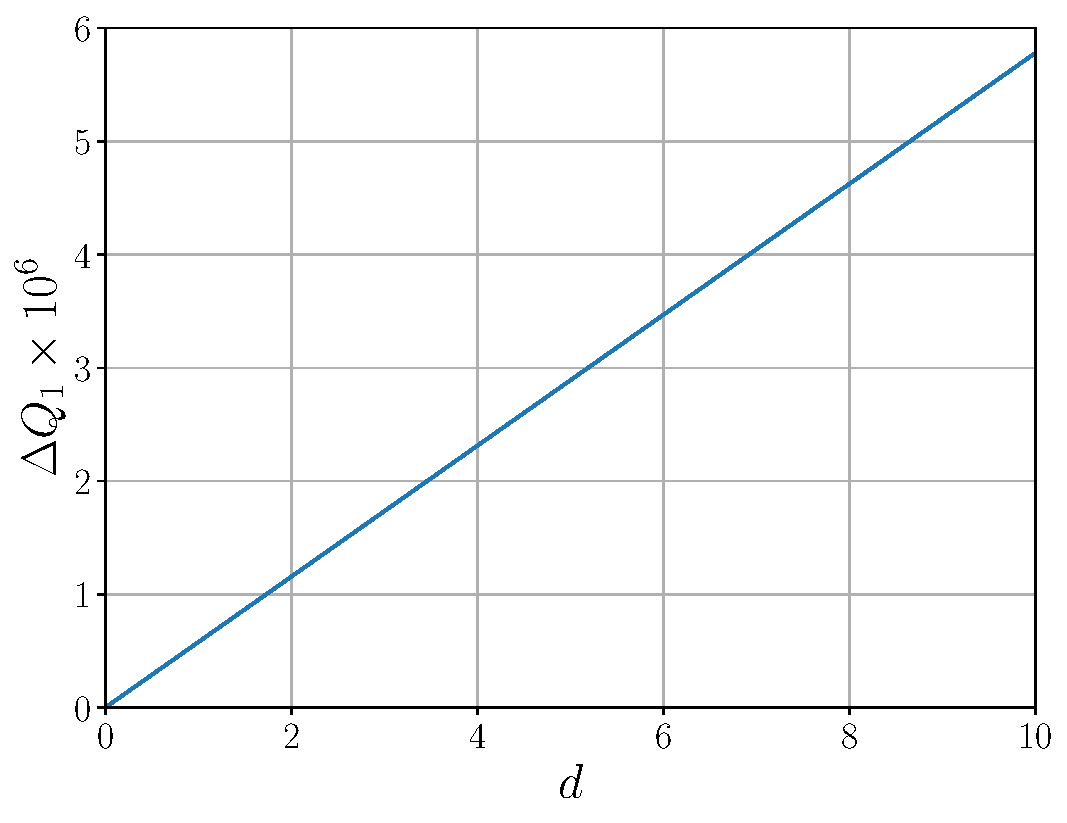
\includegraphics[width=5.0in]{../figures/fret_disp}\caption{Relative displacement $\Delta Q_1 / Q_1$}
%         \label{fig:fret_disp}
%     \end{subfigure}
%     \par\vspace{0.25in}
%     \begin{subfigure}[b]{0.8\textwidth}
%         \centering
%         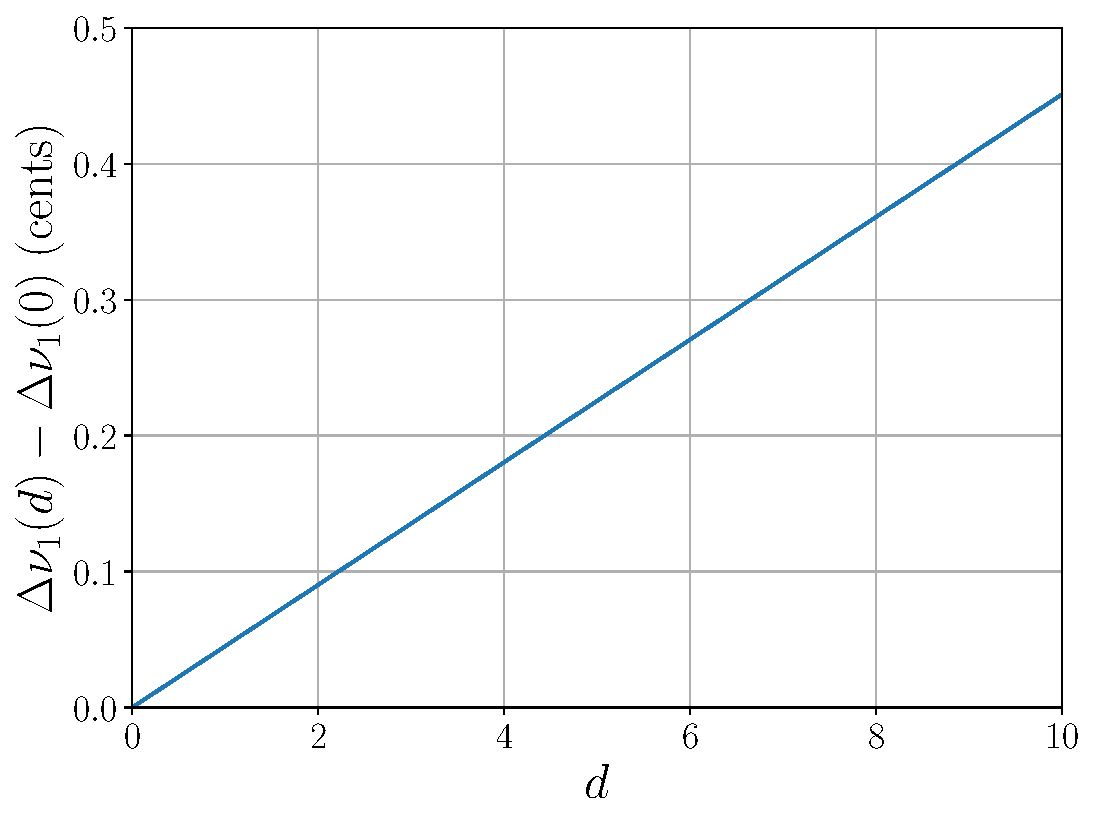
\includegraphics[width=5.0in]{../figures/fret_shift}\caption{Additional frequency shift for $\kappa = 49$}\label{fig:fret_shift}
%     \end{subfigure}
%     \caption{\label{fig:fret_model} In (a), we plot the relative displacement $\Delta Q_1 / Q_1$ for the first fret as a function of the fretting distance parameter $d$ using \eqn{delta_q_n_approx}. Here the guitar has the same parameters as the ``no-relief'' Alhambra 8P, with normal tension strings. In (b), we show the additional frequency shift given by \eqn{delta_nu_n_d} at the first fret of a string with $\kappa = 49$ as $d$ increases from 0. For $n > 1$, the relative displacement and additional shift are reduced by a factor of approximately $n^2$.}
% \end{figure}

 %%%%%%%%%%%%%%%%%%%%%%%%%%%%%%%%%%%%%%%%%%%%%%%%%%%%%%%%%%%%%%%%%%%%%%%%%%%%%%
%
% Appendix file included in main project file using \input{}
%
% Assumes that LaTeX2e macros and packages defined in cg_comp.sty are
%   available
%
%%%%%%%%%%%%%%%%%%%%%%%%%%%%%%%%%%%%%%%%%%%%%%%%%%%%%%%%%%%%%%%%%%%%%%%%%%%%%%

 \section{Compensation by Minimizing RMS Error\label{app:rms}}

The root-mean-square (RMS) frequency error (in cents) averaged over the frets $n \in \{1, n_\text{max}\}$ \emph{of a particular string} is given by
 \begin{equation}\label{eqn:rms_def}
\overline{\Delta \nu}_\text{rms} \equiv \sqrt{\frac{\sum_{n = 1}^{n_\text{max}} \Delta \nu_n^2}{n_\text{max}}}\, ,
 \end{equation}
where $\Delta \nu_n$ is given by \eqn{error_tot}. Here we will vary both $\Delta S$ and $\Delta N$ to minimize $\overline{\Delta \nu}_\text{rms}$. In this case, it is sufficient to minimize the quantity
 \begin{equation}\label{eqn:chi2_def}
\chi^2 = \sum_{n = 1}^{n_\text{max}} \left[\frac{\ln(2)}{1200}\, \Delta \nu_n\right]^2
 \end{equation}
such that the gradient of $\chi^2$ with respect to $\Delta S$ and $\Delta N$ vanishes. The components of this gradient are
 \begin{subequations}\label{chi2_grad}
 \begin{align}
\frac{\partial}{\partial \Delta S}\, \chi^2 &= -\frac{2}{X_0}\, \sum_n (\gamma_n - 1)\left[ (\gamma_n - 1) \left(B_0 - \frac{\Delta S}{X_0}\right) + \frac{\Delta N}{X_0} + \frac{\kappa}{2}\, Q_n \right]\, , \nd \\
\frac{\partial}{\partial \Delta N}\, \chi^2 &= \frac{2}{X_0}\, \sum_n \left[ (\gamma_n - 1) \left(B_0 - \frac{\Delta S}{X_0}\right) + \frac{\Delta N}{X_0} + \frac{\kappa}{2}\, Q_n \right]\, .
 \end{align}
 \end{subequations}
Setting both of these expressions to zero, we can rewrite them as the matrix equation
 \begin{equation} \label{eqn:rms_mat}
\begin{bmatrix}
  \sigma_2 & -\sigma_1 \\
  \sigma_1 & -\sigma_0
\end{bmatrix}\,
\begin{bmatrix}
  \Delta S \\
  \Delta N
\end{bmatrix} = X_0
\begin{bmatrix}
  \sigma_2\, B_0 +  \half\, \kappa\, \overline{Q}_1 \\
  \sigma_1\, B_0 +  \half\, \kappa\, \overline{Q}_0
\end{bmatrix}\, ,
 \end{equation}
where
 \begin{align}
\sigma_k &\equiv \sum_{n = 1}^{n_\text{max}} \left(\gamma_n - 1\right)^k\, , \nd \\
\overline{Q}_k &\equiv \sum_{n = 1}^{n_\text{max}} \left(\gamma_n - 1\right)^k\, Q_n\, .
 \end{align}
\Eqn{rms_mat} has the straightforward analytic solution
 \begin{equation}\label{eqn:rms_sol}
\begin{bmatrix}
  \Delta S \\
  \Delta N
\end{bmatrix} = \frac{X_0}{\sigma_1^2 - \sigma_0\, \sigma_2}\,
\begin{bmatrix}
  -\sigma_0 & \sigma_1 \\
  -\sigma_1 & \sigma_2
\end{bmatrix}\,
\begin{bmatrix}
  \sigma_2\, B_0 + \half\, \kappa\, \overline{Q}_1 \\
  \sigma_1\, B_0 + \half\, \kappa\, \overline{Q}_0
\end{bmatrix}\, .
 \end{equation}
For completeness, the corresponding solution when the quadratic stiffness term is included is given by
 \begin{equation}\label{eqn:rms_sol_quad}
\begin{bmatrix}
  \Delta S \\
  \Delta N
\end{bmatrix} = \frac{X_0}{\sigma_1^2 - \sigma_0\, \sigma_2}\,
\begin{bmatrix}
  -\sigma_0 & \sigma_1 \\
  -\sigma_1 & \sigma_2
\end{bmatrix}\,
\begin{bmatrix}
  \sigma_2\, B_0 + \half \left(1 + \pi^2\right) \left(2 \sigma_2 + \sigma_3\right) B_0^2 + \half\, \kappa\, \overline{Q}_1 \\
  \sigma_1\, B_0 + \half \left(1 + \pi^2\right) \left(2 \sigma_1 + \sigma_2\right) B_0^2 + \half\, \kappa\, \overline{Q}_0
\end{bmatrix}\, .
 \end{equation}

The corresponding Hessian matrix for this problem is
 \begin{equation}
H = \begin{bmatrix}
      \frac{\partial^2 \chi^2}{\partial \Delta S^2} & \frac{\partial^2 \chi^2}{\partial \Delta N\, \partial \Delta S} \\
      \frac{\partial^2 \chi^2}{\partial \Delta S\, \partial \Delta N} & \frac{\partial^2 \chi^2}{\partial \Delta N^2}
    \end{bmatrix}
  = \frac{2}{X_0^2} \begin{bmatrix}
      \sigma_2 & -\sigma_1 \\
      -\sigma_1 & \sigma_0
    \end{bmatrix}\, .
 \end{equation}
The Hessian is positive definite if and only if all of its eigenvalues are positive, and in the case of a $2 \times 2$ real matrix, this holds when the determinant is greater than zero. It is easy to verify numerically (and with some effort algebraically) that $\Det(H) > 0$ for $n_\text{max} > 1$. Therefore, the solution for $\Delta S$ and $\Delta N$ given by \eqn{rms_sol} minimizes the RMS frequency error.

The setback solution given by \eqn{rms_sol} is valid for a single string, and results like those shown in \tbl{ej45_setbacks} and \fig{shift_alhambra8p_ej45_full} assume that the guitar is built such that each string --- from a particular set of strings --- has a unique saddle and nut setback. Suppose that we'd prefer to engineer a guitar with single, uniform values of both $\Delta S$ and $\Delta N$ that provide reasonable compensation across an entire string set (or an ensemble of strings from a variety of manufacturers). In this case, \eqn{rms_def} becomes
 \begin{equation}\label{eqn:rms_def_m}
\overline{\Delta \nu}_\text{rms} \equiv \sqrt{\frac{\sum_{m = 1}^{m_\text{max}} \sum_{n = 1}^{n_\text{max}} \left[\Delta \nu^{(m)}_{n}\right]^2}{m_\text{max}\, n_\text{max}}}\, ,
 \end{equation}
where $m$ labels the strings in the set, and \eqn{error_tot} has been updated to become
 \begin{equation}\label{eqn:error_tot_m}
\Delta \nu^{(m)}_n \approx \frac{1200}{\ln(2)}\, \left\{ \left(\gamma_n - 1\right) \left[B_0^{(m)} - \frac{\Delta S}{X_0}\right] + \frac{\Delta N}{X_0} + \half\, \kappa^{(m)}\, Q_n \right\}\, .
 \end{equation}
If we rigorously follow the same approach that we used to arrive at \eqn{rms_sol}, in the multi-string case we obtain
 \begin{equation}\label{eqn:rms_sol_multi}
\begin{bmatrix}
  \Delta S \\
  \Delta N
\end{bmatrix} = \frac{1}{m_\text{max}}\, 
\begin{bmatrix}
  \sum_{m = 1}^{m_\text{max}} \Delta S^{(m)} \\
  \sum_{m = 1}^{m_\text{max}} \Delta N^{(m)}
\end{bmatrix}\, ,
 \end{equation}
where
 \begin{equation}\label{eqn:rms_sol_uni}
\begin{bmatrix}
  \Delta S^{(m)} \\
  \Delta N^{(m)}
\end{bmatrix} = \frac{X_0}{\sigma_1^2 - \sigma_0\, \sigma_2}\,
\begin{bmatrix}
  -\sigma_0 & \sigma_1 \\
  -\sigma_1 & \sigma_2
\end{bmatrix}\,
\begin{bmatrix}
  \sigma_2\, B_0^{(m)} + \half\, \kappa^{(m)}\, \overline{Q}_1 \\
  \sigma_1\, B_0^{(m)} + \half\, \kappa^{(m)}\, \overline{Q}_0
\end{bmatrix}\, .
 \end{equation}
In other words, we can find the optimum values for both $\Delta S$ and $\Delta N$ simply by averaging the corresponding setbacks over a commercially interesting collection of string sets. 
 %%%%%%%%%%%%%%%%%%%%%%%%%%%%%%%%%%%%%%%%%%%%%%%%%%%%%%%%%%%%%%%%%%%%%%%%%%%%%%
%
% Appendix file included in main project file using \input{}
%
% Assumes that LaTeX2e macros and packages defined in cg_comp.sty are
%   available
%
%%%%%%%%%%%%%%%%%%%%%%%%%%%%%%%%%%%%%%%%%%%%%%%%%%%%%%%%%%%%%%%%%%%%%%%%%%%%%%

 \newpage
 \section{Other Classical Guitar String Sets\label{app:specs}}

 \subsection{Light Tension -- Nylon}

% \begin{table}[htbp]
%  \centering
%  \caption{\label{tbl:ej43_ips} String specifications for the D'Addario Pro-Arte Nylon Classical Guitar Strings -- Light Tension (EJ43). The corresponding scale length is 25.5~inches.}
%    \begin{tabular}{lcccc}
%    \toprule
%    String  & Note  & \multicolumn{1}{l}{Diameter (in)} & \multicolumn{1}{l}{Density (lb/in)} & \multicolumn{1}{l}{Tension (lb)} \\
%    \midrule
%    J4301 & $E_4$  & 0.0275 & $2.024 \times 10^{-5}$ & 14.8 \\
%    J4302 & $B_3$  & 0.0317 & $2.729 \times 10^{-5}$ & 11.2 \\
%    J4303 & $G_3$  & 0.0397 & $4.525 \times 10^{-5}$ & 11.7 \\
%    J4304 & $D_3$  & 0.0280 & $1.020 \times 10^{-4}$ & 14.8 \\
%    J4305 & $A_2$  & 0.0330 & $1.535 \times 10^{-4}$ & 12.5 \\
%    J4306 & $E_2$  & 0.0420 & $2.888 \times 10^{-4}$ & 13.2 \\
%    \bottomrule
%    \end{tabular}%
% \end{table}%

 \begin{table}[htbp]
  \centering
  \caption{\label{tbl:ej43_mks} String specifications for the D'Addario Pro-Arte Nylon Classical Guitar Strings -- Light Tension (EJ43). The corresponding scale length is 650~mm.}
  \begin{tabular}{ccccc}
\toprule
String &     Note &  Radius (mm) &  Density ($\times 10^{-7}$ kg/mm) &  Tension (N) \\
\midrule
 J4301 &  E$_{4}$ &         0.35 &                              3.62 &        66.39 \\
 J4302 &  B$_{3}$ &         0.40 &                              4.87 &        50.24 \\
 J4303 &  G$_{3}$ &         0.50 &                              8.08 &        52.48 \\
 J4304 &  D$_{3}$ &         0.36 &                             18.23 &        66.41 \\
 J4305 &  A$_{2}$ &         0.42 &                             27.41 &        56.06 \\
 J4306 &  E$_{2}$ &         0.53 &                             51.59 &        59.21 \\
\bottomrule
\end{tabular}


 \end{table}%

 \begin{table}[htbp]
  \centering
  \caption{\label{tbl:ej43_props} Derived physical properties of the D'Addario Pro-Arte Nylon Classical Guitar Strings -- Light Tension (EJ43). The corresponding scale length is 650 mm.}
  \begin{tabular}{cccccc}
\toprule
String &  $\Delta \nu_{12}$ (cents) &  $R$ &  $\kappa$ &  $E$ (GPa) &  $B_0$ ($\times 10^{-3}$) \\
\midrule
 J4301 &                          2 & 23.2 &      47.3 &        8.2 &                       1.8 \\
 J4302 &                          0 & 11.2 &      23.4 &        2.3 &                       1.5 \\
 J4303 &                         10 & 55.6 &     112.2 &        7.4 &                       4.1 \\
 J4304 &                          2 & 22.8 &      46.7 &        7.8 &                       1.9 \\
 J4305 &                          3 & 24.8 &      50.5 &        5.1 &                       2.3 \\
 J4306 &                          2 & 15.5 &      32.0 &        2.1 &                       2.3 \\
\bottomrule
\end{tabular}


 \end{table}%

 \begin{table}[htbp]
  \centering
  \caption{\label{tbl:ej43_setbacks} Predicted setbacks for the D'Addario Pro-Arte Nylon Classical Guitar Strings -- Light Tension (EJ43) on the Alhambra 8P classical guitar.}
  \begin{tabular}{cccccc}
\toprule
String & $\Delta S$ (mm) & $\Delta N$ (mm) & $\overline{\Delta \nu}_\text{rms}$ (cents) \\
\midrule
J4301 & 2.01 & -0.56 & 0.25 \\
J4302 & 2.43 & -0.63 & 0.28 \\
J4303 & 3.44 & -0.81 & 0.36 \\
J4304 & 1.82 & -0.47 & 0.21 \\
J4305 & 1.88 & -0.39 & 0.18 \\
J4306 & 2.45 & -0.42 & 0.19 \\
\bottomrule
\end{tabular}


 \end{table}%

 \begin{figure}
  \centering
  \begin{subfigure}[b]{0.45\textwidth}
   \centering
   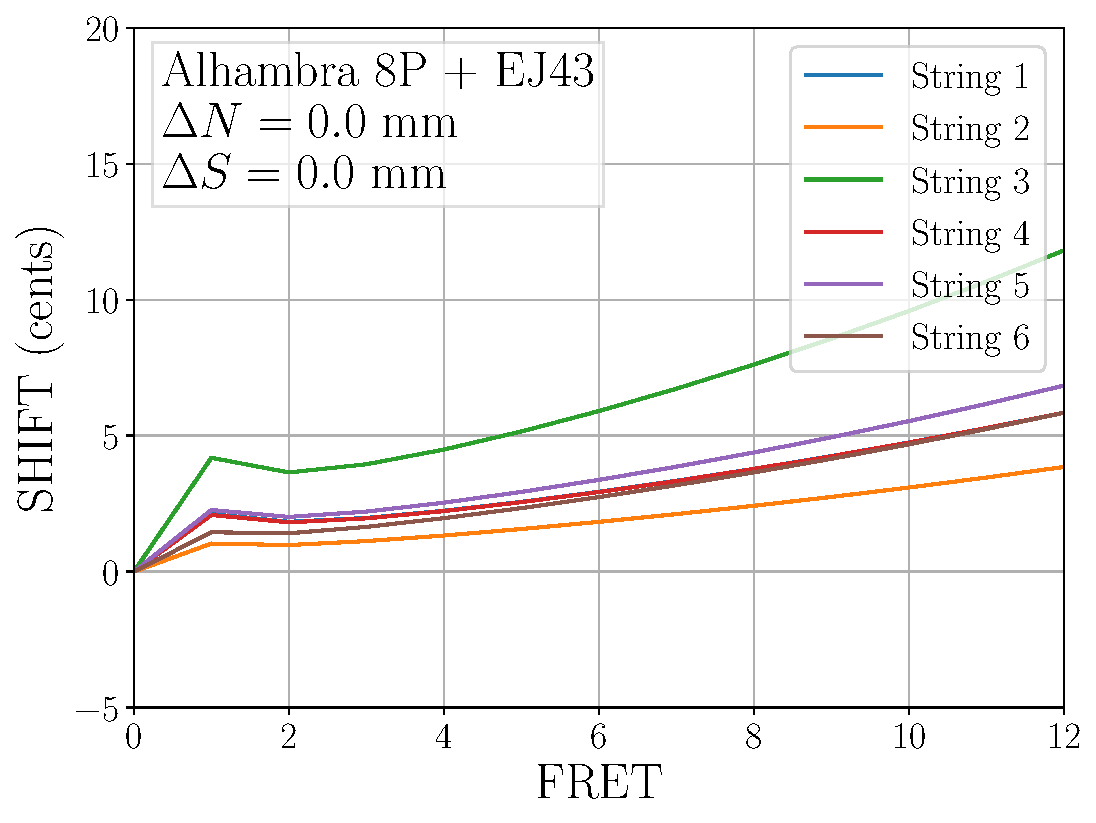
\includegraphics[width=3.25in]{../figures/shift_alhambra8p_ej43_null}
   \caption{Uncompensated}
   \label{fig:shift_alhambra8p_ej43_null}
  \end{subfigure}
  \hspace{0.25in}
  \begin{subfigure}[b]{0.45\textwidth}
   \centering
   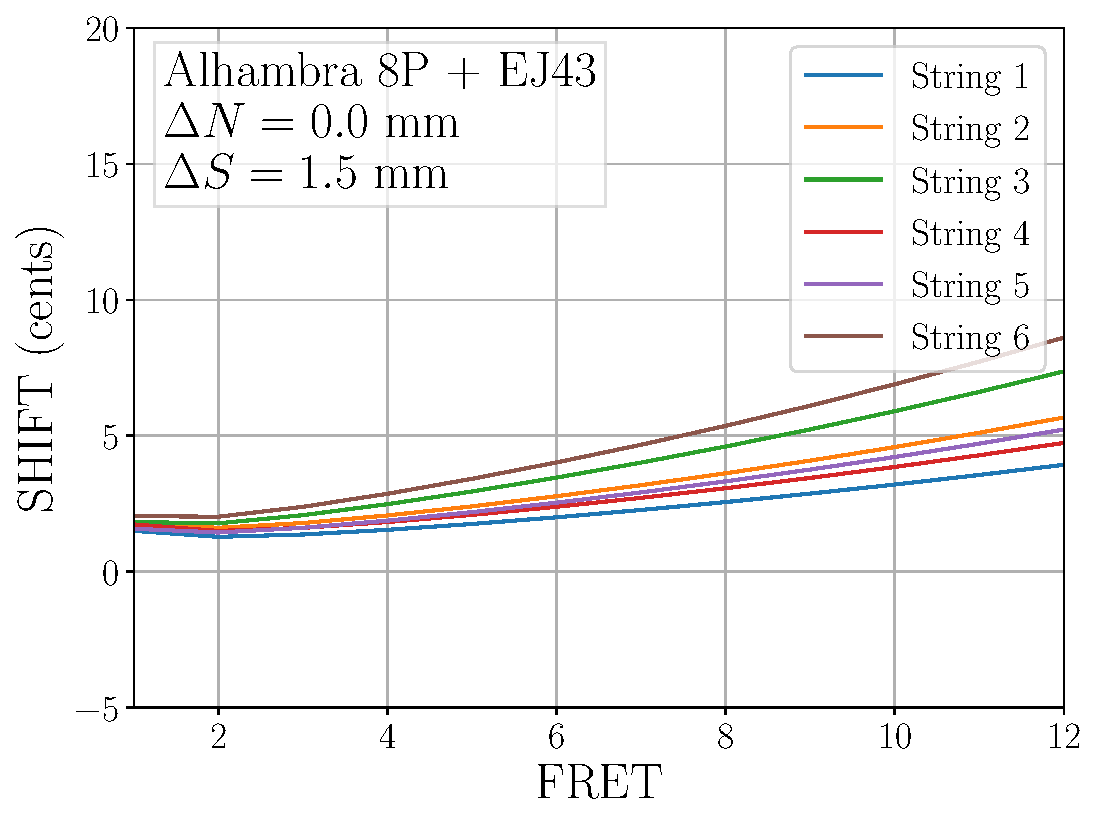
\includegraphics[width=3.25in]{../figures/shift_alhambra8p_ej43_factory}
   \caption{Factory guitar}
   \label{fig:shift_alhambra8p_ej43_factory}
  \end{subfigure}
  \par\vspace{0.25in}
  \begin{subfigure}[b]{0.45\textwidth}
   \centering
   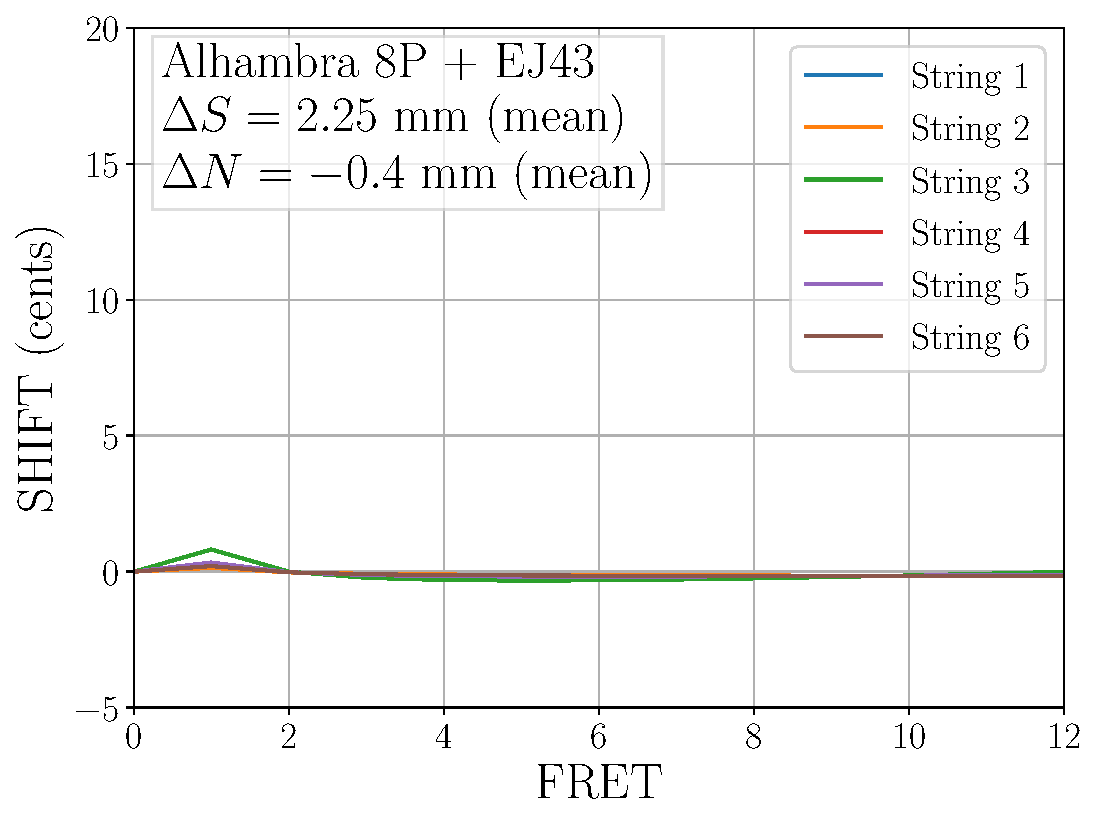
\includegraphics[width=3.25in]{../figures/shift_alhambra8p_ej43_full}
   \caption{Full compensation}
   \label{fig:shift_alhambra8p_ej43_full}
  \end{subfigure}
  \hspace{0.25in}
  \begin{subfigure}[b]{0.45\textwidth}
   \centering
   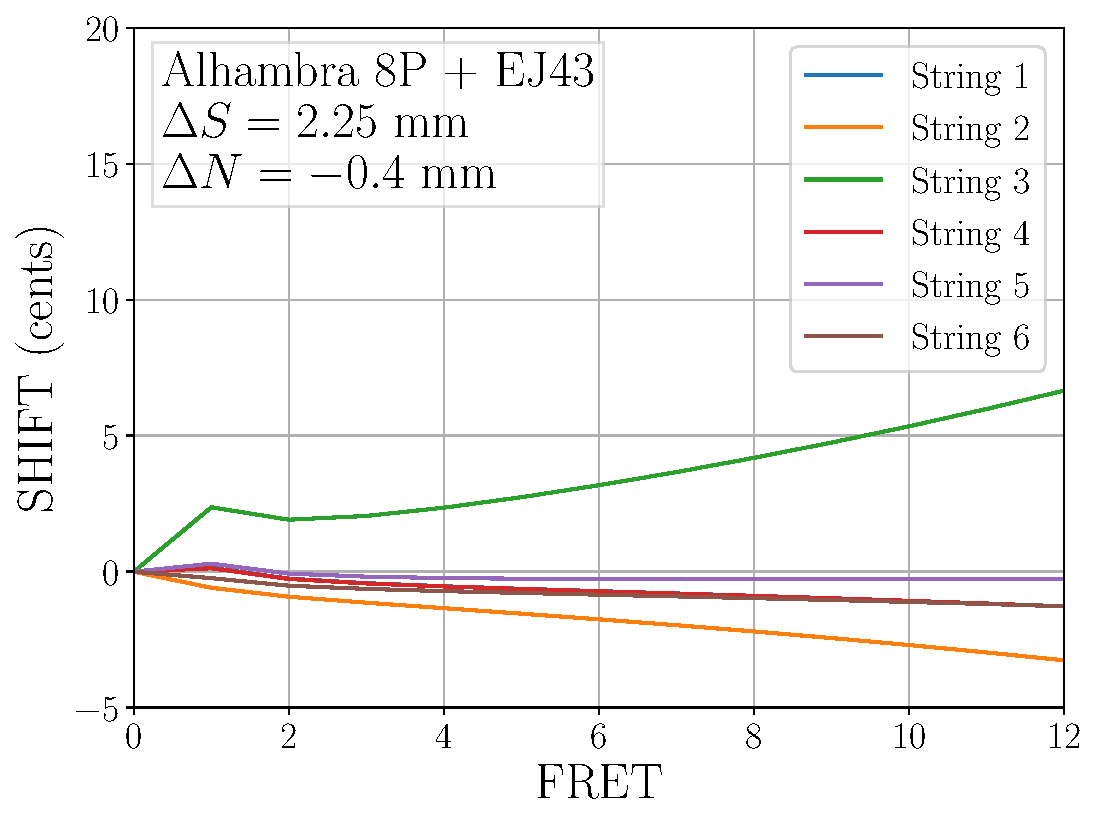
\includegraphics[width=3.25in]{../figures/shift_alhambra8p_ej43_mean}
   \caption{Mean compensation}
   \label{fig:shift_alhambra8p_ej43_mean}
  \end{subfigure}
  \caption{\label{fig:compensation_alhambra8p_ej43} Frequency shift (in cents) for an Alhambra 8P guitar with D'Addario Pro-Arte Nylon Classical Guitar Strings -- Light Tension (EJ43). Four different strategies of saddle and nut compensation are illustrated.}
 \end{figure}

 \newpage
 \subsection{Hard Tension -- Nylon}

% \begin{table}[htbp]
%  \centering
%  \caption{\label{tbl:ej46_ips} String specifications for the D'Addario Pro-Arte Nylon Classical Guitar Strings -- Hard Tension (EJ46). The corresponding scale length is 25.5~inches.}
%    \begin{tabular}{lcccc}
%    \toprule
%    String  & Note  & \multicolumn{1}{l}{Diameter (in)} & \multicolumn{1}{l}{Density (lb/in)} & \multicolumn{1}{l}{Tension (lb)} \\
%    \midrule
%    J4601 & $E_4$  & 0.0285 & $2.161 \times 10^{-5}$ & 15.8 \\
%    J4602 & $B_3$  & 0.0327 & $2.924 \times 10^{-5}$ & 12.0 \\
%    J4603 & $G_3$  & 0.0410 & $4.795 \times 10^{-5}$ & 12.4 \\
%    J4604 & $D_3$  & 0.0300 & $1.124 \times 10^{-4}$ & 16.3 \\
%    J4605 & $A_2$  & 0.0360 & $1.952 \times 10^{-4}$ & 15.9 \\
%    J4606 & $E_2$  & 0.0440 & $3.173 \times 10^{-4}$ & 14.5 \\
%    \bottomrule
%    \end{tabular}%
% \end{table}%

 \begin{table}[htbp]
  \centering
  \caption{\label{tbl:ej46_mks} String specifications for the D'Addario Pro-Arte Nylon Classical Guitar Strings -- Hard Tension (EJ46). The corresponding scale length is 650~mm.}
  \begin{tabular}{ccccc}
\toprule
String &    Note &  Radius (mm) &  Density ($\times 10^{-7}$ kg/mm) &  Tension (N) \\
\midrule
 J4601 & E$_{4}$ &         0.36 &                              3.86 &        70.88 \\
 J4602 & B$_{3}$ &         0.42 &                              5.22 &        53.83 \\
 J4603 & G$_{3}$ &         0.52 &                              8.57 &        55.61 \\
 J4604 & D$_{3}$ &         0.38 &                             20.07 &        73.14 \\
 J4605 & A$_{2}$ &         0.46 &                             34.87 &        71.31 \\
 J4606 & E$_{2}$ &         0.56 &                             56.67 &        65.04 \\
\bottomrule
\end{tabular}


 \end{table}%

 \begin{table}[htbp]
  \centering
  \caption{\label{tbl:ej46_props} Derived physical properties of the D'Addario Pro-Arte Nylon Classical Guitar Strings -- Hard Tension (EJ46).}
%  \caption{\label{tbl:ej46_props} Derived physical properties of the D'Addario Pro-Arte Nylon Classical Guitar Strings -- Hard Tension (EJ46). Note that the estimated value of $R$ seems anomalously high for String 1 (E) compared to other D'Addario string sets.}
  \begin{tabular}{cccccc}
\toprule
String &  $\Delta \nu_{12}$ (cents) &  $R$ ($\times 10^4$) &  $\kappa$ &  $E$ (GPa) &  $B_0$ ($\times 10^{-3}$) \\
\midrule
 J4601 &                          3 &                 12.2 &     139.8 &       24.1 &                       3.3 \\
 J4602 &                          2 &                  6.3 &      71.9 &        7.1 &                       2.7 \\
 J4603 &                         10 &                  5.2 &      59.4 &        3.9 &                       3.1 \\
 J4604 &                          0 &                  6.7 &      76.6 &       12.3 &                       2.6 \\
 J4605 &                          2 &                  3.3 &      37.5 &        4.1 &                       2.2 \\
 J4606 &                          4 &                  4.9 &      55.5 &        3.7 &                       3.2 \\
\bottomrule
\end{tabular}


 \end{table}%

 \begin{table}[htbp]
  \centering
  \caption{\label{tbl:ej46_setbacks} Predicted setbacks for the D'Addario Pro-Arte Nylon Classical Guitar Strings -- Hard Tension (EJ46) on the Alhambra 8P classical guitar.}
%  \caption{\label{tbl:ej46_setbacks} Predicted setbacks for the D'Addario Pro-Arte Nylon Classical Guitar Strings -- Hard Tension (EJ46) on the Alhambra 8P classical guitar. The high $R$ value listed for String 1 in \tbl{ej46_props} leads to large setbacks.}
  \begin{tabular}{cccccc}
\toprule
String & $\Delta S$ (mm) & $\Delta N$ (mm) & $\overline{\Delta \nu}_\text{rms}$ (cents) \\
\midrule
J4601 & 1.55 & -0.35 & 0.16 \\
J4602 & 1.87 & -0.39 & 0.18 \\
J4603 & 2.39 & -0.42 & 0.19 \\
J4604 & 1.59 & -0.34 & 0.16 \\
J4605 & 1.93 & -0.36 & 0.17 \\
J4606 & 2.40 & -0.38 & 0.18 \\
\bottomrule
\end{tabular}


 \end{table}%

 \begin{figure}
  \centering
  \begin{subfigure}[b]{0.45\textwidth}
   \centering
   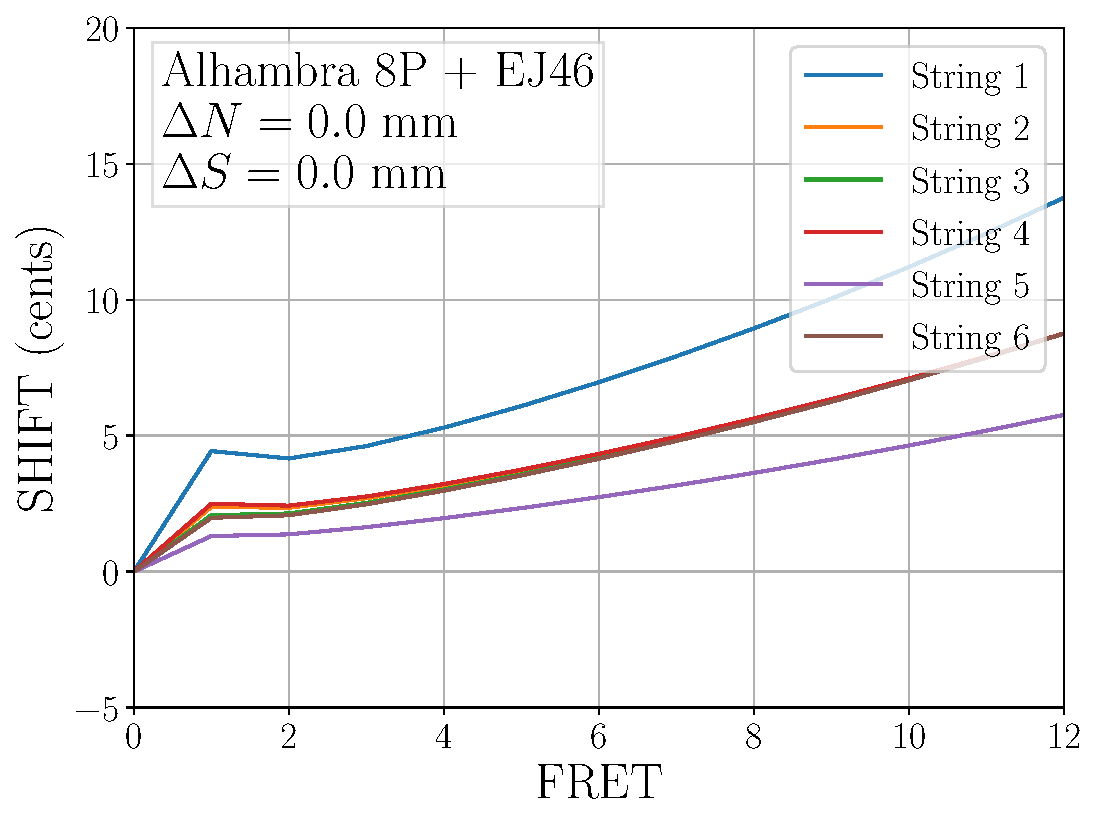
\includegraphics[width=3.25in]{../figures/shift_alhambra8p_ej46_null}
   \caption{Uncompensated}
   \label{fig:shift_alhambra8p_ej46_null}
  \end{subfigure}
  \hspace{0.25in}
  \begin{subfigure}[b]{0.45\textwidth}
   \centering
   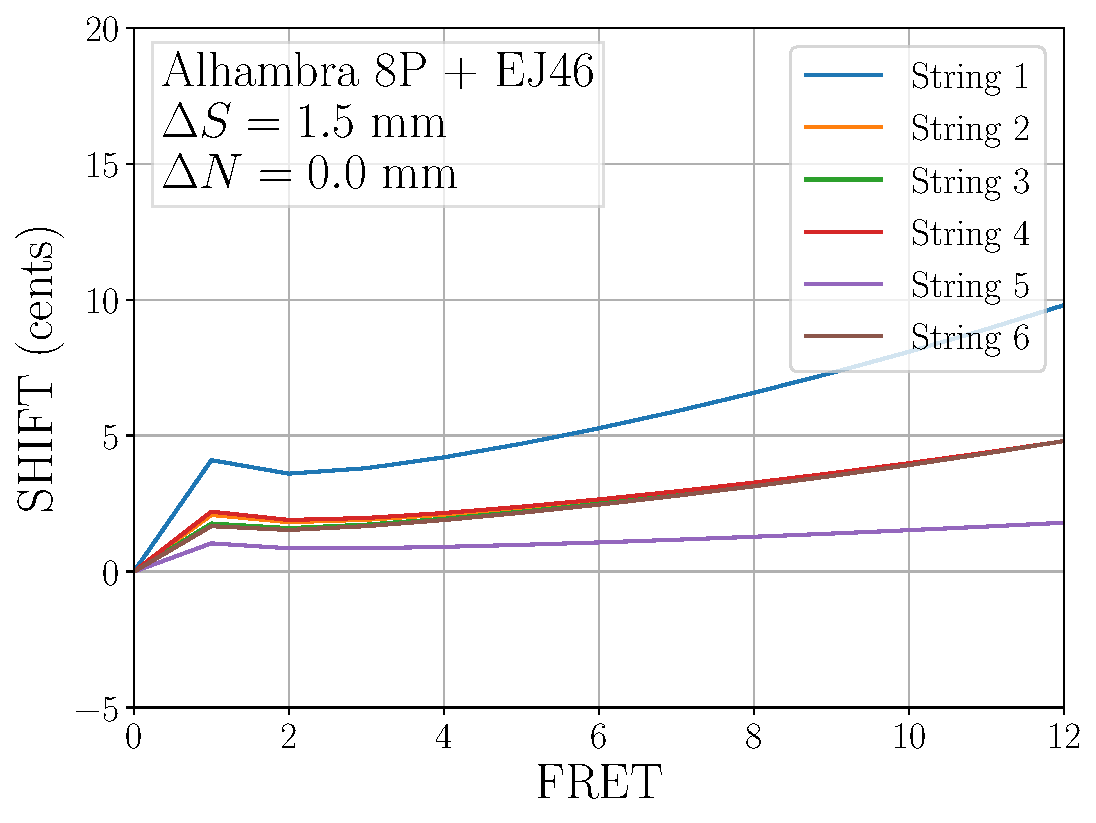
\includegraphics[width=3.25in]{../figures/shift_alhambra8p_ej46_factory}
   \caption{Factory guitar}
   \label{fig:shift_alhambra8p_ej46_factory}
  \end{subfigure}
  \par\vspace{0.25in}
  \begin{subfigure}[b]{0.45\textwidth}
   \centering
   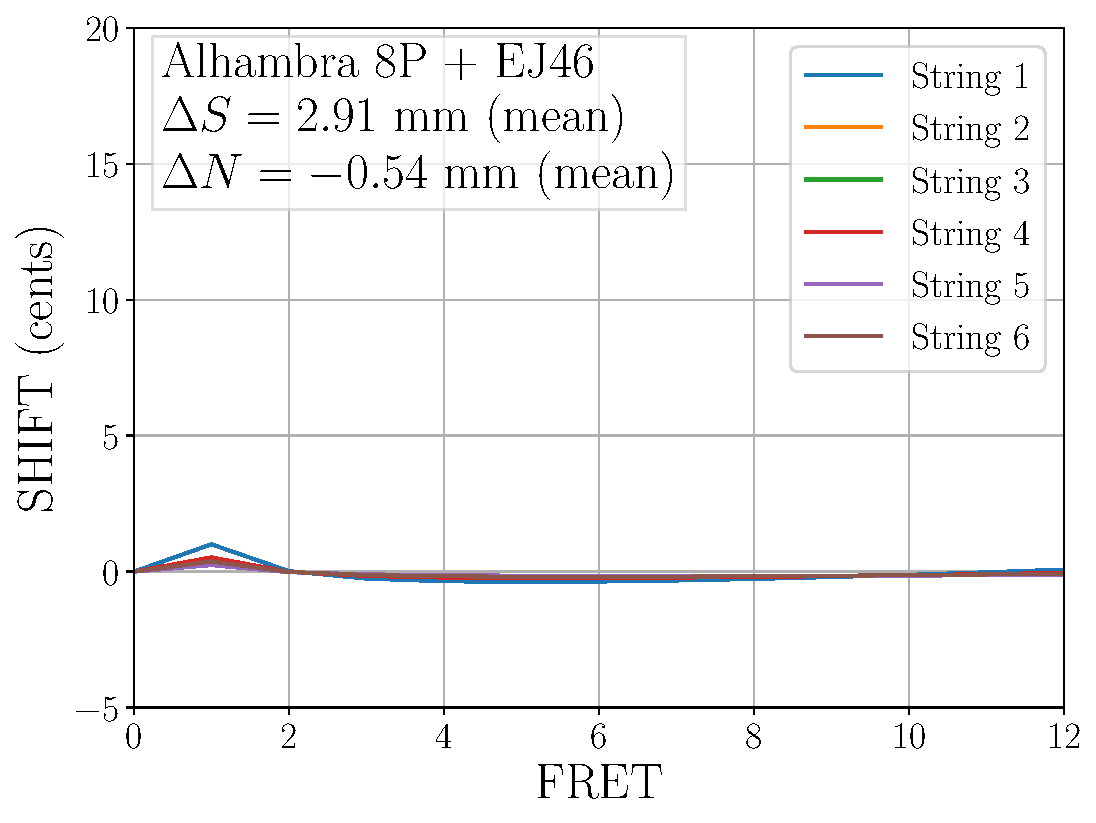
\includegraphics[width=3.25in]{../figures/shift_alhambra8p_ej46_full}
   \caption{Full compensation}
   \label{fig:shift_alhambra8p_ej46_full}
  \end{subfigure}
  \hspace{0.25in}
  \begin{subfigure}[b]{0.45\textwidth}
   \centering
   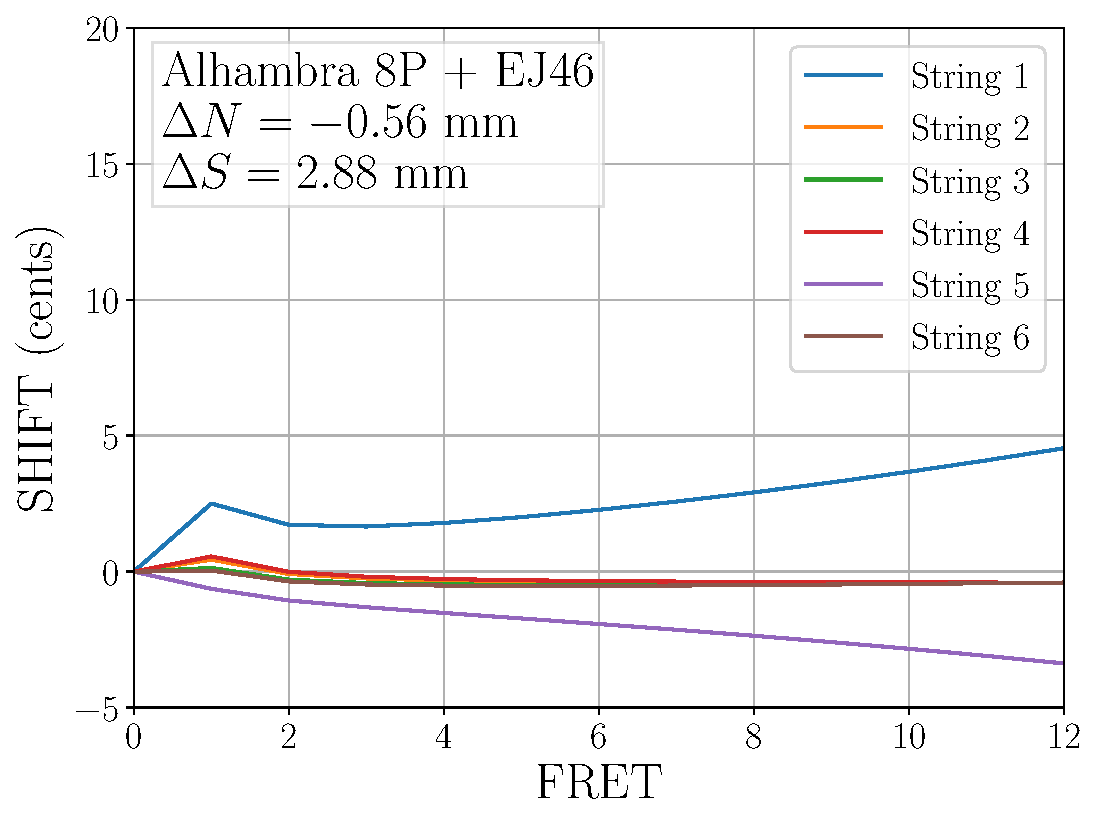
\includegraphics[width=3.25in]{../figures/shift_alhambra8p_ej46_mean}
   \caption{Mean compensation}
   \label{fig:shift_alhambra8p_ej46_mean}
  \end{subfigure}
  \caption{\label{fig:compensation_alhambra8p_ej46} Frequency shift (in cents) for an Alhambra 8P guitar with D'Addario Pro-Arte Nylon Classical Guitar Strings -- Hard Tension (EJ46). Four different strategies of saddle and nut compensation are illustrated.}
 \end{figure}

 \newpage
 \subsection{Extra Hard Tension -- Nylon}

% \begin{table}[htbp]
%  \centering
%  \caption{\label{tbl:ej44_ips} String specifications for the D'Addario Pro-Arte Nylon Classical Guitar Strings -- Extra Hard Tension (EJ44). The corresponding scale length is 25.5~inches.}
%    \begin{tabular}{lcccc}
%    \toprule
%    String  & Note  & \multicolumn{1}{l}{Diameter (in)} & \multicolumn{1}{l}{Density (lb/in)} & \multicolumn{1}{l}{Tension (lb)} \\
%    \midrule
%    J4401 & $E_4$  & 0.0290 & $2.243 \times 10^{-5}$ & 16.4 \\
%    J4402 & $B_3$  & 0.0333 & $3.046 \times 10^{-5}$ & 12.5 \\
%    J4403 & $G_3$  & 0.0416 & $4.989 \times 10^{-5}$ & 12.9 \\
%    J4404 & $D_3$  & 0.0300 & $1.124 \times 10^{-4}$ & 16.3 \\
%    J4405 & $A_2$  & 0.0360 & $1.952 \times 10^{-4}$ & 15.9 \\
%    J4406 & $E_2$  & 0.0450 & $3.435 \times 10^{-4}$ & 15.7 \\
%    \bottomrule
%    \end{tabular}%
% \end{table}%

 \begin{table}[htbp]
  \centering
  \caption{\label{tbl:ej44_mks} String specifications for the D'Addario Pro-Arte Nylon Classical Guitar Strings -- Extra Hard Tension (EJ44). The corresponding scale length is 650~mm.}
  \begin{tabular}{ccccc}
\toprule
String &   Note &  Radius (mm) &  Density ($\times 10^{-7}$ kg/mm) &  Tension (N) \\
\midrule
 J4401 &  $E_4$ &         0.37 &                              4.01 &        73.57 \\
 J4402 &  $B_3$ &         0.42 &                              5.44 &        56.07 \\
 J4403 &  $G_3$ &         0.53 &                              8.91 &        57.86 \\
 J4404 &  $D_3$ &         0.38 &                             20.07 &        73.14 \\
 J4405 &  $A_2$ &         0.46 &                             34.87 &        71.31 \\
 J4406 &  $E_2$ &         0.57 &                             61.36 &        70.42 \\
\bottomrule
\end{tabular}


 \end{table}%

 \begin{table}[htbp]
  \centering
  \caption{\label{tbl:ej44_props} Derived physical properties of the D'Addario Pro-Arte Nylon Classical Guitar Strings -- Extra Hard Tension (EJ44). The corresponding scale length is 650 mm.}
  \begin{tabular}{cccccc}
\toprule
String &  $\Delta \nu_{12}$ (cents) &  $R$ ($\times 10^4$) &  $\kappa$ &  $E$ (GPa) &  $B_0$ ($\times 10^{-3}$) \\
\midrule
 J4401 &                          3 &                  4.0 &      45.4 &        7.8 &                       1.9 \\
 J4402 &                          2 &                  8.1 &      92.7 &        9.3 &                       3.1 \\
 J4403 &                         10 &                  9.5 &     108.2 &        7.1 &                       4.2 \\
 J4404 &                          0 &                  6.7 &      76.6 &       12.3 &                       2.6 \\
 J4405 &                          2 &                  3.3 &      37.5 &        4.1 &                       2.2 \\
 J4406 &                          4 &                  4.8 &      54.3 &        3.7 &                       3.2 \\
\bottomrule
\end{tabular}


 \end{table}%

 \begin{table}[htbp]
  \centering
  \caption{\label{tbl:ej44_setbacks} Predicted setbacks for the D'Addario Pro-Arte Nylon Classical Guitar Strings -- Extra Hard Tension (EJ44) on the Alhambra 8P classical guitar.}
  \begin{tabular}{cccc}
\toprule
String &  $\Delta S$ (mm) &  $\Delta N$ (mm) &  $\overline{\Delta \nu}_\text{rms}$ (cents) \\
\midrule
 J4401 &             1.89 &            -0.34 &                                        0.16 \\
 J4402 &             3.38 &            -0.69 &                                        0.26 \\
 J4403 &             4.39 &            -0.80 &                                        0.30 \\
 J4404 &             2.76 &            -0.57 &                                        0.22 \\
 J4405 &             1.95 &            -0.28 &                                        0.15 \\
 J4406 &             2.94 &            -0.40 &                                        0.17 \\
\bottomrule
\end{tabular}


 \end{table}%

 \begin{figure}
  \centering
  \begin{subfigure}[b]{0.45\textwidth}
   \centering
   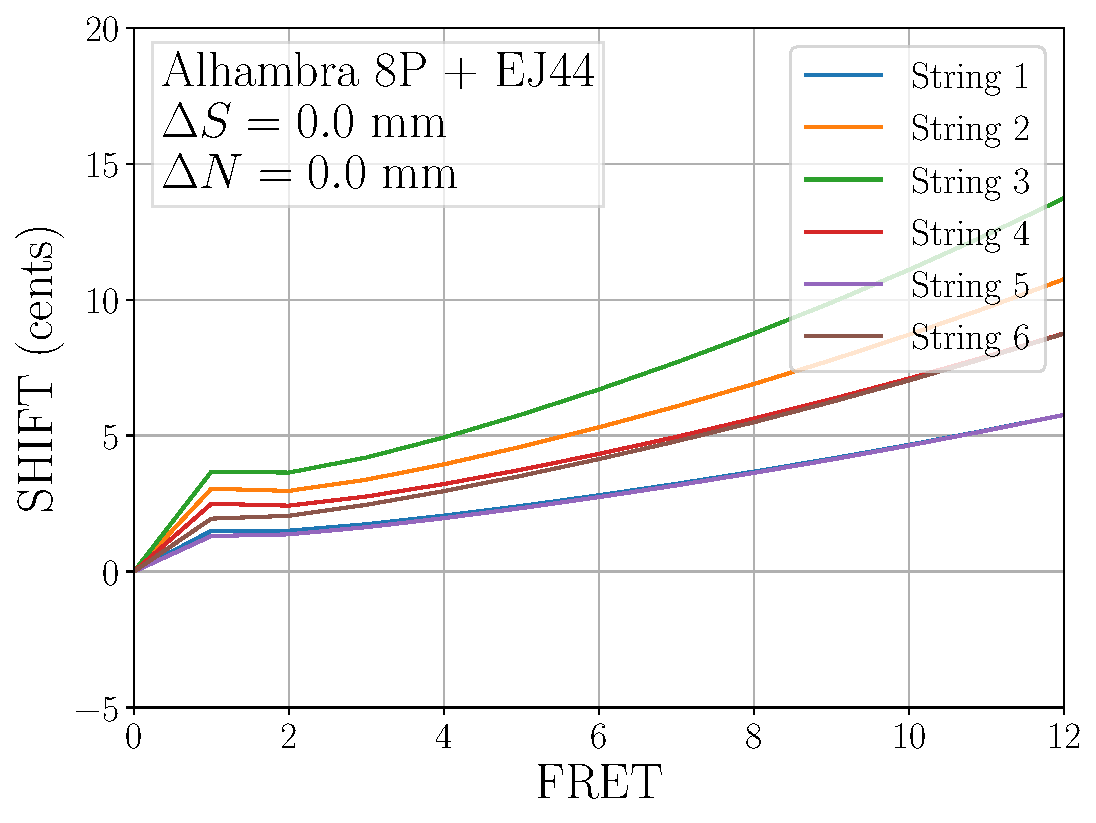
\includegraphics[width=3.25in]{../figures/shift_alhambra8p_ej44_null}
   \caption{Uncompensated}
   \label{fig:shift_alhambra8p_ej44_null}
  \end{subfigure}
  \hspace{0.25in}
  \begin{subfigure}[b]{0.45\textwidth}
   \centering
   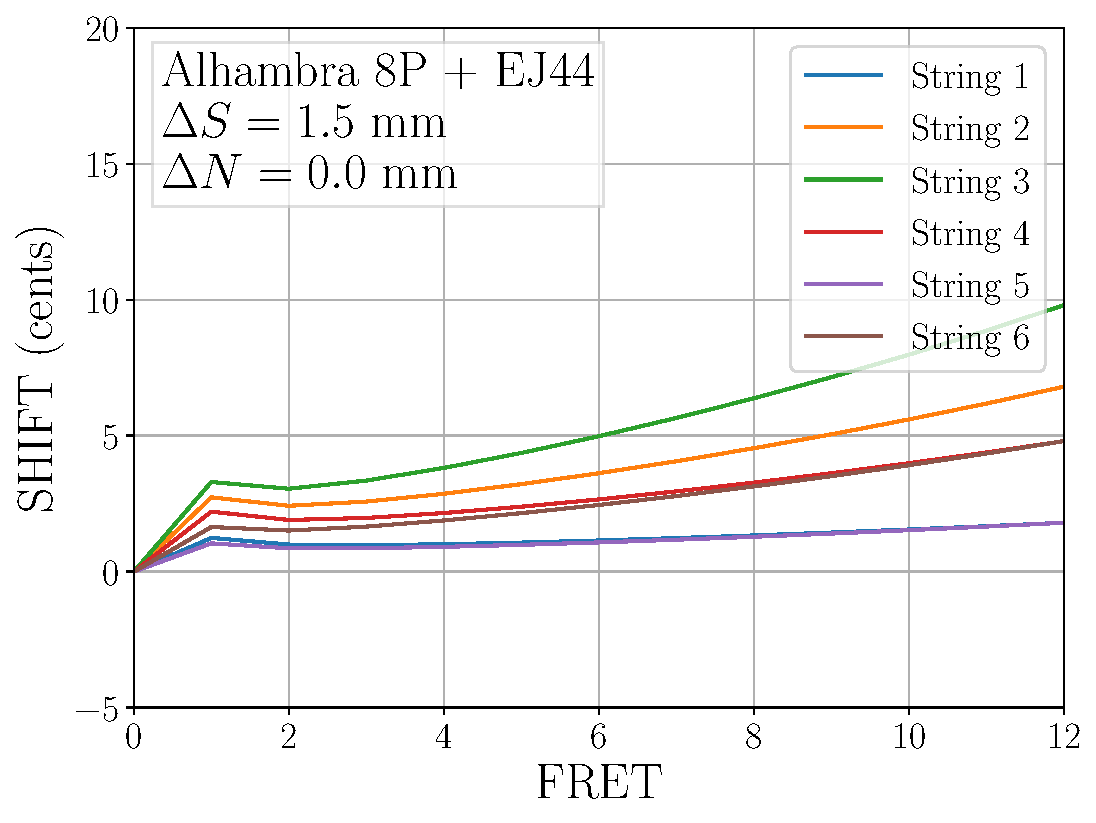
\includegraphics[width=3.25in]{../figures/shift_alhambra8p_ej44_factory}
   \caption{Factory guitar}
   \label{fig:shift_alhambra8p_ej44_factory}
  \end{subfigure}
  \par\vspace{0.25in}
  \begin{subfigure}[b]{0.45\textwidth}
   \centering
   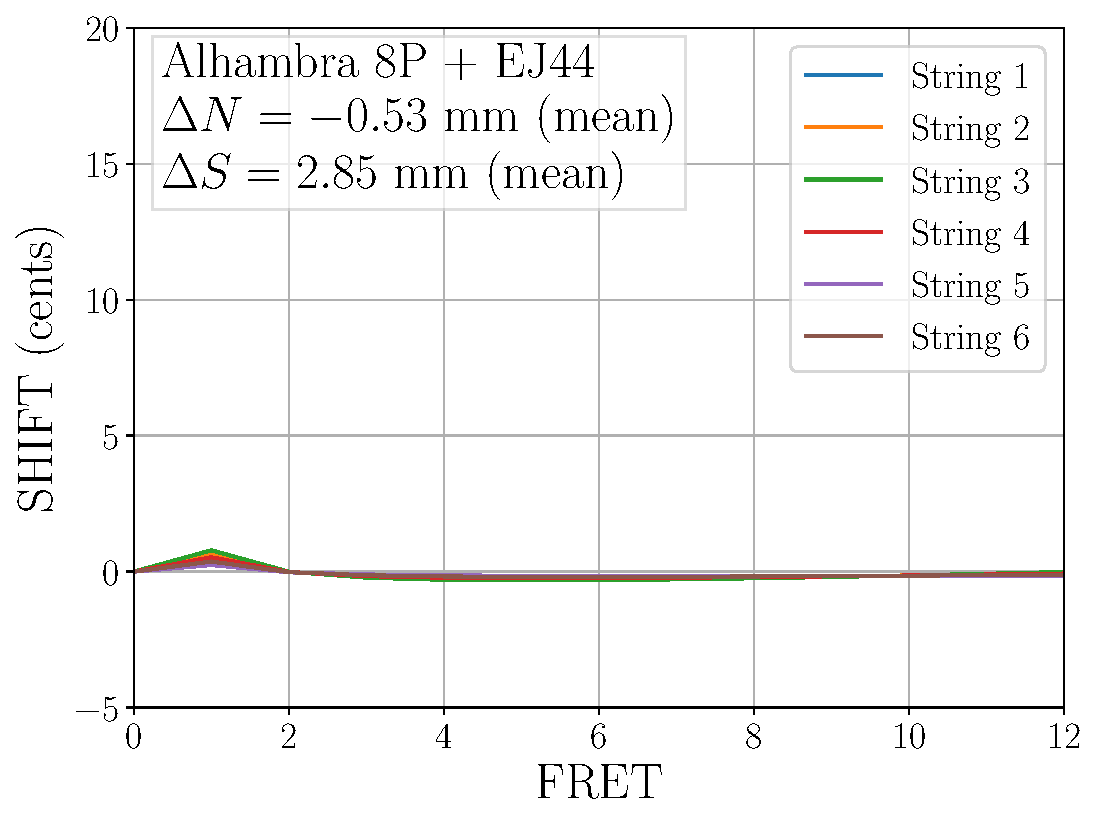
\includegraphics[width=3.25in]{../figures/shift_alhambra8p_ej44_full}
   \caption{Full compensation}
   \label{fig:shift_alhambra8p_ej44_full}
  \end{subfigure}
  \hspace{0.25in}
  \begin{subfigure}[b]{0.45\textwidth}
   \centering
   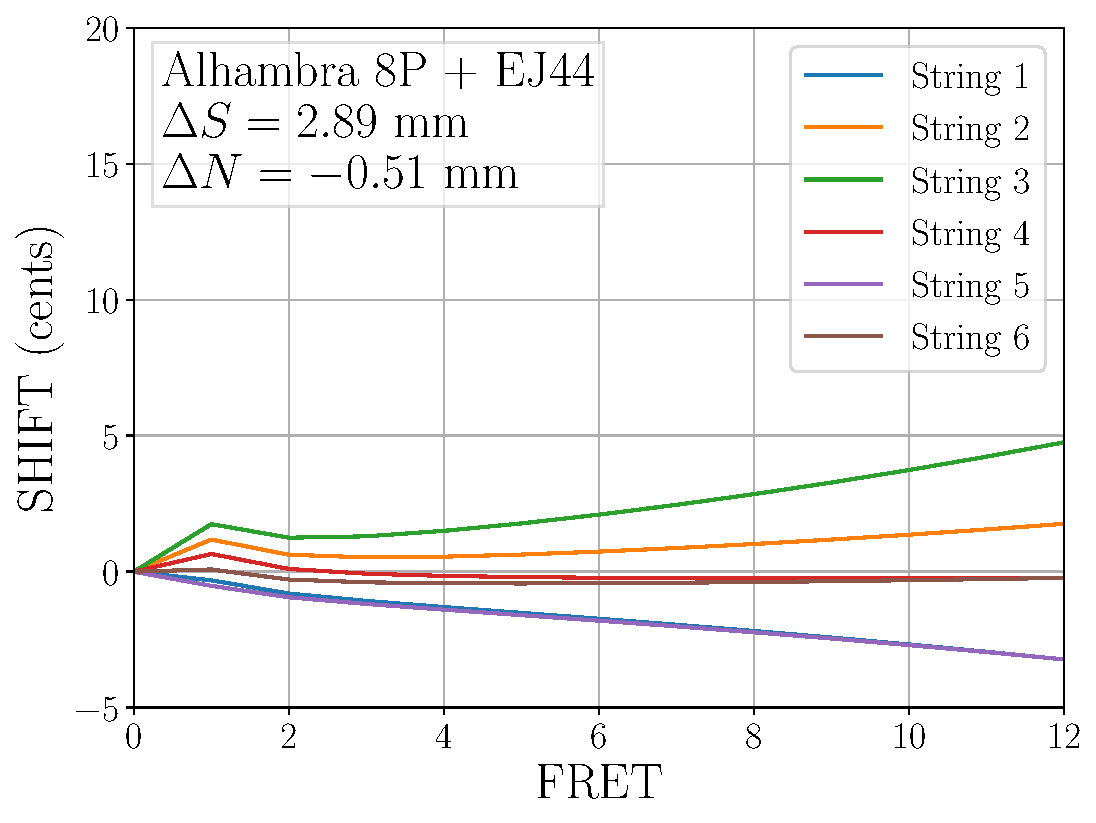
\includegraphics[width=3.25in]{../figures/shift_alhambra8p_ej44_mean}
   \caption{Mean compensation}
   \label{fig:shift_alhambra8p_ej44_mean}
  \end{subfigure}
  \caption{\label{fig:compensation_alhambra8p_ej44} Frequency shift (in cents) for an Alhambra 8P guitar with D'Addario Pro-Arte Nylon Classical Guitar Strings -- Extra Hard Tension (EJ44). Four different strategies of saddle and nut compensation are illustrated.}
 \end{figure}

 \newpage
 \subsection{Normal Tension -- Carbon}
 
 \begin{table}[htbp]
   \centering
   \caption{\label{tbl:ej45ff_mks} String specifications for the D'Addario Pro-Arte Carbon Classical Guitar Strings -- Normal Tension (EJ45FF). The corresponding scale length is 650~mm.}
   \begin{tabular}{cccccc}
\toprule
String & Note & Radius (mm) & Density ($\times 10^{-7}$ kg/mm) & Tension (N) \\
\midrule
J4501FF & E$_{4}$ & 0.305 & 4.64 & 85.3 \\
J4502FF & B$_{3}$ & 0.345 & 6.07 & 62.6 \\
J4503FF & G$_{3}$ & 0.420 & 8.93 & 58.0 \\
J4504FF & D$_{3}$ & 0.356 & 16.43 & 59.9 \\
J4505FF & A$_{2}$ & 0.445 & 30.90 & 63.2 \\
J4506FF & E$_{2}$ & 0.559 & 57.16 & 65.6 \\
\bottomrule
\end{tabular}


 \end{table}%
 
 \begin{table}[htbp]
   \centering
   \caption{\label{tbl:ej45ff_props} Derived physical properties of the D'Addario Pro-Arte Carbon Classical Guitar Strings -- Normal Tension (EJ45FF). The corresponding scale length is 650 mm.}
   \begin{tabular}{cccccc}
\toprule
String & $R$ & $\sigma$ & $\kappa$ & $B_0$ & $E$ (GPa) \\
\midrule
J4501FF & 21.8 & 0.4 & 44.6 & 0.00157 & 13.04 \\
J4502FF & 26.0 & 0.6 & 53.1 & 0.00194 & 8.86 \\
J4503FF & 26.9 & 0.8 & 54.7 & 0.00239 & 5.71 \\
J4504FF & 24.3 & 0.4 & 49.6 & 0.00193 & 7.47 \\
J4505FF & 26.9 & 0.4 & 54.7 & 0.00253 & 5.57 \\
J4506FF & 23.5 & 0.9 & 47.9 & 0.00298 & 3.20 \\
\bottomrule
\end{tabular}


 \end{table}%
 
 \begin{table}[htbp]
   \centering
   \caption{\label{tbl:ej45ff_setbacks} Predicted setbacks for the D'Addario Pro-Arte Carbon Classical Guitar Strings -- Normal Tension (EJ45FF) on the Alhambra 8P classical guitar.}
   \begin{tabular}{cccccc}
\toprule
String & $\Delta S$ (mm) & $\Delta N$ (mm) & $\overline{\Delta \nu}_\text{rms}$ (cents) \\
\midrule
J4501FF & 1.23 & -0.26 & 0.13 \\
J4502FF & 1.51 & -0.31 & 0.15 \\
J4503FF & 1.84 & -0.32 & 0.15 \\
J4504FF & 1.49 & -0.29 & 0.14 \\
J4505FF & 1.93 & -0.32 & 0.15 \\
J4506FF & 2.22 & -0.28 & 0.14 \\
\bottomrule
\end{tabular}


 \end{table}%
 
 \begin{figure}
   \centering
   \begin{subfigure}[b]{0.46\textwidth}
    \centering
    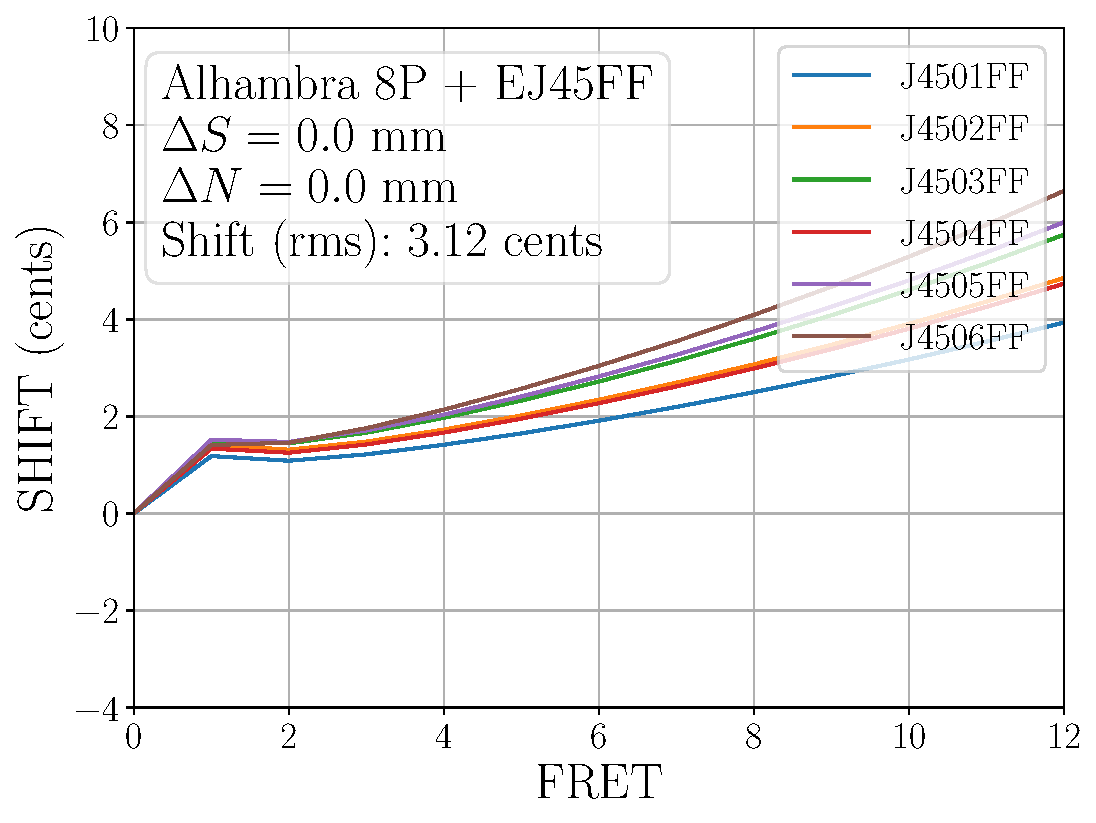
\includegraphics[width=3.25in]{../figures/shift_alhambra8p_ej45ff_null}
    \caption{Uncompensated}
    \label{fig:shift_alhambra8p_ej45ff_null}
   \end{subfigure}
   \hspace{0.25in}
   \begin{subfigure}[b]{0.46\textwidth}
    \centering
    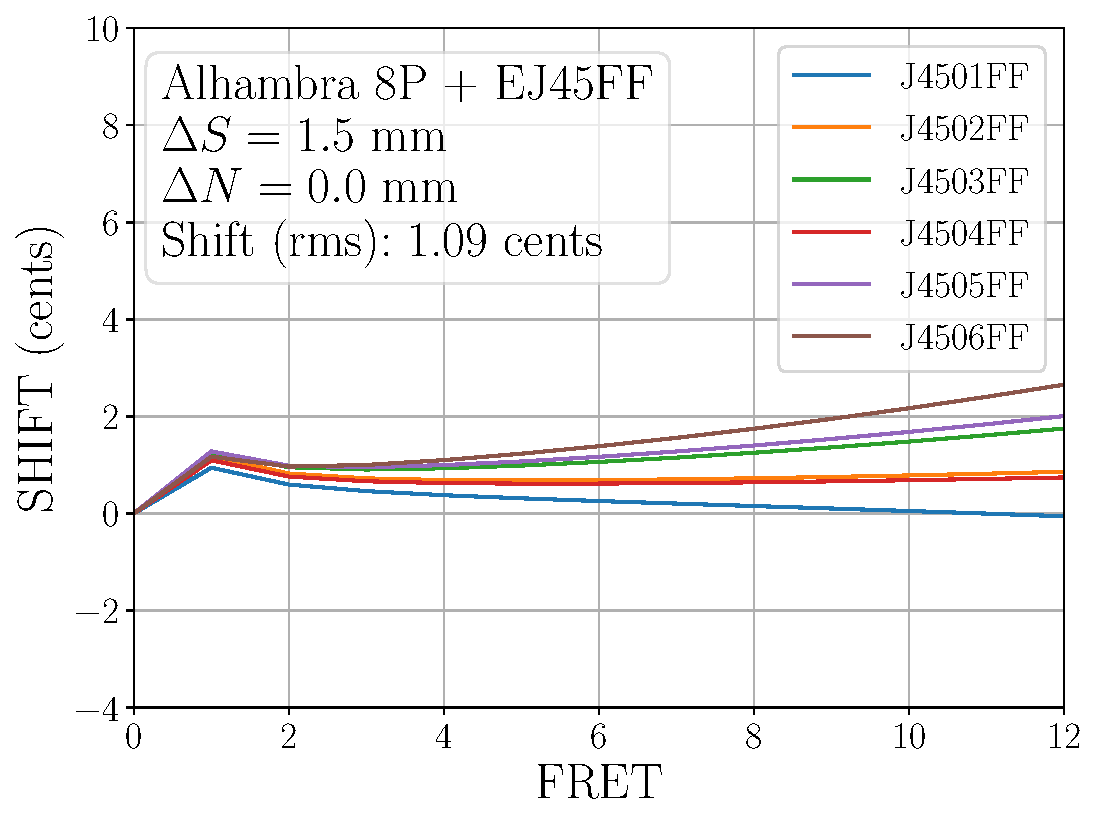
\includegraphics[width=3.25in]{../figures/shift_alhambra8p_ej45ff_factory}
    \caption{Factory guitar}
    \label{fig:shift_alhambra8p_ej45ff_factory}
   \end{subfigure}
   \par\vspace{0.25in}
   \begin{subfigure}[b]{0.46\textwidth}
    \centering
    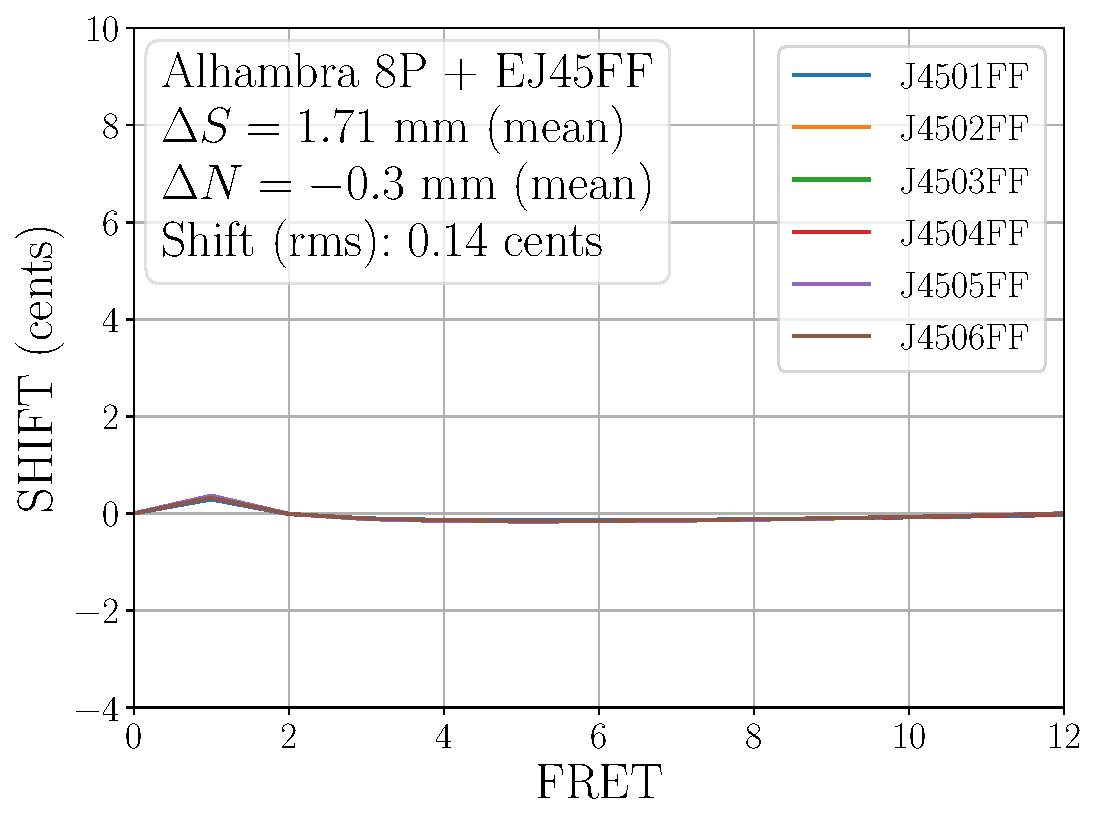
\includegraphics[width=3.25in]{../figures/shift_alhambra8p_ej45ff_full}
    \caption{Full compensation}
    \label{fig:shift_alhambra8p_ej45ff_full}
   \end{subfigure}
   \hspace{0.25in}
   \begin{subfigure}[b]{0.46\textwidth}
    \centering
    \includegraphics[width=3.25in]{../figures/shift_alhambra8p_ej45ff_mean}
    \caption{Mean compensation}
    \label{fig:shift_alhambra8p_ej45ff_mean}
   \end{subfigure}
   \caption{\label{fig:compensation_alhambra8p_ej45ff} Frequency shift (in cents) for an Alhambra 8P guitar with D'Addario Pro-Arte Carbon Classical Guitar Strings -- Normal Tension (EJ45FF). Four different strategies of saddle and nut compensation are illustrated.}
 \end{figure}
 
 \newpage
 \subsection{Hard Tension -- Carbon}
 
 \begin{table}[htbp]
   \centering
   \caption{\label{tbl:ej46ff_mks} String specifications for the D'Addario Pro-Arte Carbon Classical Guitar Strings -- Hard Tension (EJ46FF). The corresponding scale length is 650~mm.}
   \begin{tabular}{cccccc}
\toprule
String & Note & Radius (mm) & Density ($\times 10^{-7}$ kg/mm) & Tension (N) \\
\midrule
J4501FF & E$_{4}$ & 0.305 & 4.64 & 85.3 \\
J4502FF & B$_{3}$ & 0.345 & 6.07 & 62.6 \\
J4503FF & G$_{3}$ & 0.420 & 8.93 & 58.0 \\
J4504FF & D$_{3}$ & 0.356 & 16.43 & 59.9 \\
J4505FF & A$_{2}$ & 0.445 & 30.90 & 63.2 \\
J4506FF & E$_{2}$ & 0.559 & 57.16 & 65.6 \\
\bottomrule
\end{tabular}


 \end{table}%
 
 \begin{table}[htbp]
   \centering
   \caption{\label{tbl:ej46ff_props} Derived physical properties of the D'Addario Pro-Arte Carbon Classical Guitar Strings -- Hard Tension (EJ46FF). The corresponding scale length is 650 mm.}
   \begin{tabular}{cccccc}
\toprule
String & $R$ & $\sigma$ & $\kappa$ & $B_0$ & $E$ (GPa) \\
\midrule
J4601FF & 22.2 & 0.3 & 45.4 & 0.00163 & 13.39 \\
J4602FF & 23.1 & 0.4 & 47.1 & 0.00188 & 7.86 \\
J4603FF & 25.8 & 0.6 & 52.6 & 0.00240 & 5.55 \\
J4604FF & 23.1 & 0.4 & 47.2 & 0.00195 & 7.43 \\
J4605FF & 23.8 & 0.2 & 48.6 & 0.00245 & 5.38 \\
J4606FF & 23.1 & 0.4 & 47.2 & 0.00309 & 3.09 \\
\bottomrule
\end{tabular}


 \end{table}%
 
 \begin{table}[htbp]
   \centering
   \caption{\label{tbl:ej46ff_setbacks} Predicted setbacks for the D'Addario Pro-Arte Carbon Classical Guitar Strings -- Hard Tension (EJ46FF) on the Alhambra 8P classical guitar.}
   \begin{tabular}{cccccc}
\toprule
String & $\Delta S$ (mm) & $\Delta N$ (mm) & $\overline{\Delta \nu}_\text{rms}$ (cents) \\
\midrule
J4601FF & 1.34 & -0.33 & 0.16 \\
J4602FF & 1.52 & -0.35 & 0.16 \\
J4603FF & 1.91 & -0.39 & 0.18 \\
J4604FF & 1.56 & -0.35 & 0.16 \\
J4605FF & 1.92 & -0.36 & 0.17 \\
J4606FF & 2.36 & -0.34 & 0.16 \\
\bottomrule
\end{tabular}


 \end{table}%
 
 \begin{figure}
   \centering
   \begin{subfigure}[b]{0.46\textwidth}
    \centering
    \includegraphics[width=3.25in]{../figures/shift_alhambra8p_ej46ff_null}
    \caption{Uncompensated}
    \label{fig:shift_alhambra8p_ej46ff_null}
   \end{subfigure}
   \hspace{0.25in}
   \begin{subfigure}[b]{0.46\textwidth}
    \centering
    \includegraphics[width=3.25in]{../figures/shift_alhambra8p_ej46ff_factory}
    \caption{Factory guitar}
    \label{fig:shift_alhambra8p_ej46ff_factory}
   \end{subfigure}
   \par\vspace{0.25in}
   \begin{subfigure}[b]{0.46\textwidth}
    \centering
    \includegraphics[width=3.25in]{../figures/shift_alhambra8p_ej46ff_full}
    \caption{Full compensation}
    \label{fig:shift_alhambra8p_ej46ff_full}
   \end{subfigure}
   \hspace{0.25in}
   \begin{subfigure}[b]{0.46\textwidth}
    \centering
    \includegraphics[width=3.25in]{../figures/shift_alhambra8p_ej46ff_mean}
    \caption{Mean compensation}
    \label{fig:shift_alhambra8p_ej46ff_mean}
   \end{subfigure}
   \caption{\label{fig:compensation_alhambra8p_ej46ff} Frequency shift (in cents) for an Alhambra 8P guitar with D'Addario Pro-Arte Carbon Classical Guitar Strings -- Hard Tension (EJ46FF). Four different strategies of saddle and nut compensation are illustrated.}
 \end{figure}
 


 \addtotoc{\refname}
 \bibliographystyle{rgb}
 \bibliography{music,cg_comp}

 \end{document}
